% !TeX encoding=utf8
% !TeX program = pdflatex
% !TeX spellcheck = de_DE
% !BIB = biber

%% Bug fixes and other packages to be loaded before the class
\RequirePackage{fix-cm} % permit Computer Modern fonts at arbitrary sizes.
%
%% Document Class (Koma Script) -----------------------------------------
%% Doc: scrguien.pdf
\documentclass[%
   %draft=true,     % draft mode (no images, layout errors shown)
   draft=false,     % final mode 
%%% --- Paper Settings ---
   paper=a4,% [Todo: add alternatives]
   paper=portrait, % landscape
   pagesize=auto, % driver
%%% --- Base Font Size ---
   fontsize=12pt,%
%%% --- Koma Script Version ---
   version=last, %
%%% --- Global Package Options ---
   ngerman, % language (passed to babel and other packages)
            % (ngerman, english, french, ...)
]{scrbook} % Classes: scrartcl, scrreprt, scrbook

% ~~~~~~~~~~~~~~~~~~~~~~~~~~~~~~~~~~~~~~~~~~~~~~~~~~~~~~~~~~~~~~~~~~~~~~~~
% Must be loaded first!
% ~~~~~~~~~~~~~~~~~~~~~~~~~~~~~~~~~~~~~~~~~~~~~~~~~~~~~~~~~~~~~~~~~~~~~~~~
% packages to allow more \write outputs
% Description: see http://www.tex.ac.uk/cgi-bin/texfaq2html?label=noroom
%   short summery: The e-TeX extensions do not help with the 
%                  "no room for a new \write" problem, but in other cases
%                  of "no room for a new <thing> "
%                  "It is essential that you load etex before any other packages, 
%                  and reserve any extra inserts immediately:"
\usepackage{etex} 
\reserveinserts{28}

% Description: Package scrwfile provides a general change of the LaTeX kernel, 
%              that solve problems with the 
%              error "no room for a new \write"
% Incompatible: titletoc (bot redefine the LaTeX kernel and are incompatible by design)
% Doc: scrguien.pdf
%
%% If titletoc is not required, the usage of this package is recommended!
% see: http://tex.stackexchange.com/questions/155101/scrwfile-removes-partial-toc-created-with-titletoc
%  
% \usepackage{scrwfile}

% Description: This package is meant to be a solution for the 
%              error "no room for a new \write"
% Note: it is less efficent than scrwfile, but the best alternative
% Doc: morewrites.pdf
\usepackage{morewrites}





% packages required for the template
\usepackage{atveryend} % must be loaded before etoolbox. (bugfix for pageslts)
\usepackage{codesection}
\usepackage{templatetools}

% ~~~~~~~~~~~~~~~~~~~~~~~~~~~~~~~~~~~~~~~~~~~~~~~~~~~~~~~~~~~~~~~~~~~~~~~~
% encoding
% ~~~~~~~~~~~~~~~~~~~~~~~~~~~~~~~~~~~~~~~~~~~~~~~~~~~~~~~~~~~~~~~~~~~~~~~~

% automatic selection of encoding
% insert chars for umlaut a and sz
\usepackage{selinput}
\SelectInputMappings{adieresis={ä},germandbls={ß},Euro={€}} 

% Encoding of _files and directories_
% (ensures that any file can be loaded without problems)
\usepackage[%
   extendedchars, encoding, multidot, space,
   filenameencoding=latin1, % Windows XP, Vista, 7
   % filenameencoding=utf8,   % Linux, OS X
]{grffile}

% ~~~~~~~~~~~~~~~~~~~~~~~~~~~~~~~~~~~~~~~~~~~~~~~~~~~~~~~~~~~~~~~~~~~~~~~~
% preamble
% ~~~~~~~~~~~~~~~~~~~~~~~~~~~~~~~~~~~~~~~~~~~~~~~~~~~~~~~~~~~~~~~~~~~~~~~~

%% select/load fonts
% ~~~~~~~~~~~~~~~~~~~~~~~~~~~~~~~~~~~~~~~~~~~~~~~~~~~~~~~~~~~~~~~~~~~~~~~~
% Fonts Fonts Fonts
% ~~~~~~~~~~~~~~~~~~~~~~~~~~~~~~~~~~~~~~~~~~~~~~~~~~~~~~~~~~~~~~~~~~~~~~~~

% Make PDF files searchable and copyable
% load before: fontenc
\usepackage{cmap} 

% T1 Schrift Encoding
\usepackage[T1]{fontenc} 

% Description: Additional Symbols (Text Companion font extension)
% Doc: encguide.pdf
\usepackage{textcomp}   

% DO NOT LOAD ae Package as a font !

%% ==== Font Families / Font Combinations  (Sans + Serif) ================

%% - Latin Modern (LaTeX Standard)
%\usepackage{lmodern}
%% sans math, use with '\mathversion{sans}'
%\IfPackageLoaded{lmodern}{\DeclareMathVersion{sans}
% Math letters from Latin Modern Sans
\SetSymbolFont{letters}{sans}{OML}{cmbr}{m}{it}
% Math operators
\SetSymbolFont{operators}{sans}{OT1}{lmss}{m}{n}
% Math symbols
\SetSymbolFont{symbols}{sans}{OMS}{lmsy}{m}{n}
% Large symbols
\SetMathAlphabet{\mathrm}{sans}{OT1}{lmr}{m}{n}
\SetMathAlphabet{\mathsf}{sans}{OT1}{lmss}{m}{n}
\SetMathAlphabet{\mathit}{sans}{OT1}{lmr}{m}{it}
}

%% -------------------
%
%% - Times, Helvetica, Courier (Word Standard...)
\usepackage{mathptmx}                 %% --- Times (incl math)
%\usepackage[scaled=.90]{helvet}       %% --- Helvetica (Arial)
%\usepackage{courier}                  %% --- Courier
%% -------------------
%%
%% - Palantino , Helvetica, Courier
%\usepackage{mathpazo}                 %% --- Palantino (incl math)
%\usepackage[scaled=.95]{helvet}       %% --- Helvetica (Arial)
%\usepackage{courier}                  %% --- Courier
%% -------------------
%
%% - Charter, Bera Sans
%\usepackage{charter}\linespread{1.05} %% --- Charter
%\renewcommand{\sfdefault}{fvs}        %% --- Bera Sans
%\usepackage[charter]{mathdesign}      %% --- Charter (Math)
%\usepackage[scaled=0.85]{luximono}    %% --- Luxi Mono (Typewriter)
%% Note: There is a better Charter font by Linotype 
%%       called 'ITC Charter'
%% -------------------

%% - URW Garamond
%\renewcommand{\rmdefault}{ugm}         %% --- URW Garamond
%\renewcommand{\sfdefault}{fvs}         %% --- Bera Sans
%%%\usepackage[small]{eulervm}            %% --- EulerVM (MATH)
%\usepackage[garamond]{mathdesign}    %% --- Garamond (Math)
%\usepackage[scaled=0.85]{luximono}    %% --- Luxi Mono (Typewriter)
%% Note:  If you can efford it, combine with commercial 
%%        sans fonts like: Syntax, Frutiger or Thesis 
%%        (but then also use the commercial Garamond ...)
%% -------------------


%%%% =========== Typewriter =============

%\usepackage{courier}                   %% --- Courier
%\renewcommand{\ttdefault}{cmtl}        %% --- CmBright Typewriter Font
%\usepackage[scaled=0.9]{luximono}      %% --- Luxi Mono (Typewriter)
%\usepackage{ulgothic}                  %% --- Letter Gothic 

%%%% =========== Math fonts ================

%% Recommanded to use with fonts: Aldus, Garamond, Melior, Sabon
%\usepackage[                           %% --- EulerVM (MATH)
%   small,       %for smaller Fonts
%  euler-digits % digits in euler fonts style
%]{eulervm}

%% combine with utopia, garamond or charter font
%\usepackage[
%%   utopia,
%%   garamond,
%%   charter
%]{mathdesign}



%%% ==== Font Families / Font Combinations  (Sans + Serif) ==========

%% - MininPro/MyriadPro
%% load after textcomp, amsmath and MnSymbol
\IfFileExists{MinionPro.sty}{
%
\ExecuteAfterPackage{amsmath}{
% Minion Pro
\usepackage[%
%%% Font selection
  %smallfamily, % (std) use only regular and bold face
  medfamily,    % use semibold face in addition to smallfamily
  %fullfamily,  % use medium face in addition to medfamily
  noopticals,   % (std) use only the optical size Text
  %opticals     % use the optical sizes Caption, Text, Subhead, and Display
  %slides,      % use only the optical size Caption (useful for slides)
  normalsize,   % (std) adapt optical sizes to the normal font size 
  %nonormalsize,% use static settings for the optical sizes
  % onlytext,   % only change the text fonts
  % onlymath,   % only change the math fonts
%%% Figure selection
  % textosf,    % use text figures in text mode
  % mathosf,    % use text figures in math mode
  % osf,        % (std) use text figures in text and math mode
  % textlf,     % use lining figures in text mode
  % mathlf,     % use lining figures in math mode
  lf,,          % use lining figures in text and math mode
  mathtabular,  % use tabular figures in math mode
%%% Miscellaneous options
  % scaled=1.0, % scale the font size by <factor>
%  minionint,    % take the integral symbols from MyriadPro, not from MnSymbol
]{MinionPro}
} % end of ExecuteAfter
%
% file not found:
}{\PackageWarning{template}{File 'MinionPro.sty' not found!\MessageBreak}{}}  %% --- MinionPro
%\IfFileExists{MyriadPro.sty}{
% load after textcomp, amsmath and MnSymbol
\ExecuteAfterPackage{amsmath}{
%% Myriad Math Fonts 
%\usepackage[onlysansmath]{MdSymbol}
%
\usepackage[%
%%% Font selection
  % smallfamily, % (std) use only regular and bold face
  medfamily,   % use semibold face in addition to smallfamily
  onlytext,    % only change the text fonts
  % onlymath   % only change the math fonts
  sansmath,     % provide math version sans and sansbold 
%%% Figure selection
  % textosf, % use text figures in text mode
  % mathosf, % use text figures in math mode
  % osf,       % (std) use text figures in text and math mode
  textlf,  % use lining figures in text mode
  mathlf,    % use lining figures in math mode
  % lf,      % use lining figures in text and math mode
  mathtabular, % use tabular figures in math mode
%%% Miscellaneous options
  % scaled=1.0, % scale the font size by <factor>
]{MyriadPro}[2012/01/07 v0.1c]

} % end of ExecuteAfter
%
% file not found:
}{\PackageWarning{template}{File 'MyriadPro.sty' not found!\MessageBreak}{}}

% set bold to medium bold by default
\renewcommand{\bfdefault}{sb}

%% If you want to use MyriadPro as your mainfont:
% \renewcommand{\familydefault}{\sfdefault}  %% --- MyriadPro
%\usepackage[scaled=0.85]{luximono} %% --- Luxi Mono (Typewriter)
%% -------------------

%% - Minion / Myriad
%\renewcommand{\rmdefault}{pmnx}   % Minion
%%\renewcommand{\rmdefault}{pmnj}  % Minion ()oldstyle digits)
%\renewcommand{\sfdefault}{pmy}    % Myriad
%% Minion Math Fonts 
%\ExecuteAfterPackage{amsmath}{\usepackage{MnSymbol}}
%% -------------------

%% ===== serif ( commercial fonts ) ================================

%% --- Adobe Aldus
%\renewcommand{\rmdefault}{pasx}
%\renewcommand{\rmdefault}{pasj} %%oldstyle digits
% math recommended: \usepackage[small]{eulervm}

%% --- Adobe Garamond
%\usepackage[garamond]{mathdesign}
%\usepackage[%
%   osf,        % oldstyle digits
%   scaled=1.05 %appropriate in many cases
%]{xagaramon}


% math recommended: \usepackage{eulervm}

%% --- Adobe Stempel Garamond
%\renewcommand{\rmdefault}{pegx}
%\renewcommand{\rmdefault}{pegj} %%oldstyle digits
%\usepackage[garamond]{mathdesign}

%% --- Adobe Melior
%\renewcommand{\rmdefault}{pml}
% math recommended: %\usepackage{eulervm}

%% --- Adobe Minion
%\renewcommand{\rmdefault}{pmnx}
%\renewcommand{\rmdefault}{pmnj} %oldstyle digits
% math recommended: \usepackage[small]{eulervm} or \usepackage{mathpmnt} % commercial
%\usepackage{MnSymbol}
%\renewcommand{\bfdefault}{sb}

%% --- Adobe Sabon
%\renewcommand{\rmdefault}{psbx}
%\renewcommand{\rmdefault}{psbj} %oldstyle digits
% math recommended: \usepackage{eulervm}

%% --- Adobe Times
% math recommended: \usepackage{mathptmx} % load first !
%\renewcommand{\rmdefault}{ptmx}
%\renewcommand{\rmdefault}{ptmj} %oldstyle digits

%% --- Linotype ITC Charter
%\renewcommand{\rmdefault}{lch}
%\usepackage[charter]{mathdesign}


%% --- Linotype Meridien
%\renewcommand{\rmdefault}{lmd}

%%% ===== sans serif (commercial fonts ) ============================

%% --- Adobe Frutiger
%\usepackage[
%   scaled=0.90
%]{frutiger}

%% --- Adobe Futura (=Linotype FuturaLT) : Sans Serif
%\usepackage[
%   scaled=0.94  % appropriate in many cases
%]{futura}

%% --- Adobe Gill Sans : Sans Serif
%\usepackage{gillsans}

%% -- Adobe Myriad  : Sans Serif
%\renewcommand{\sfdefault}{pmy}
%\renewcommand{\sfdefault}{pmyc} %% condensed Font

%% --- Syntax : sans serif font
%\usepackage[
%   scaled
%]{asyntax}

%% --- Adobe Optima : Semi Sans Serif
%\usepackage[
%   medium %darker medium weight fonts
%]{optima}

%% --- Linotype ITC Officina Sans
%\renewcommand{\sfdefault}{lo9}


%% load packages
% !TeX encoding=utf8
% !TeX program = pdflatex
% !TeX spellcheck = de-DE

%% -- package section selections -->
\DefineCodeSection[true]{PackagesBase}
\DefineCodeSection[true]{PackagesBugfixes}
\DefineCodeSection[true]{PackagesFonts}
\DefineCodeSection[true]{PackagesDiagrams}
\DefineCodeSection[true]{PackagesMath}
\DefineCodeSection[true]{PackagesScience}
\DefineCodeSection[true]{PackagesSymbols}
\DefineCodeSection[true]{PackagesTables}
\DefineCodeSection[true]{PackagesText}
\DefineCodeSection[true]{PackagesQuotes}
\DefineCodeSection[true]{PackagesCitation}
\DefineCodeSection[true]{PackagesFigures}
\DefineCodeSection[true]{PackagesCaptions}
\DefineCodeSection[true]{PackagesIndexes}
\DefineCodeSection[true]{PackagesMisc}
\DefineCodeSection[true]{PackagesVerbatim}
\DefineCodeSection[true]{PackagesFancy}
\DefineCodeSection[true]{PackagesLayout}
\DefineCodeSection[true]{PackagesHeadFoot}
\DefineCodeSection[true]{PackagesHeadings}
\DefineCodeSection[true]{PackagesTOC}
\DefineCodeSection[true]{PackagesPDF}
\DefineCodeSection[true]{PackagesAdditional}
%% <--------------------------------

% ~~~~~~~~~~~~~~~~~~~~~~~~~~~~~~~~~~~~~~~~~~~~~~~~~~~~~~~~~~~~~~~~~~~~~~~~
% These packages must be loaded before all others
% (primarily because they are required by other packages)
% ~~~~~~~~~~~~~~~~~~~~~~~~~~~~~~~~~~~~~~~~~~~~~~~~~~~~~~~~~~~~~~~~~~~~~~~~
\BeginCodeSection{PackagesBase}

% Description: Calculation with LaTeX 
% Doc: calc.pdf
\usepackage{calc}

% Description: Multi Language support for LaTeX
% Doc: babel.pdf
\usepackage{babel}
% Description: support automatic translations
% Doc: beameruserguide.pdf
\usepackage{translator}


% Description: Color support with color mixing modells
% Doc: xcolor.pdf
\usepackage[
  dvipsnames, % Load a set of predefined colors 
  table,      % Load the colortbl package
  % fixpdftex,  % Load the pdfcolmk package (may be problematic)
  hyperref,   % Support  the  hyperref  package
  fixinclude, % Prevent dvips color reset before .eps file inclusion
]{xcolor}

% Description: Support for graphics in LaTeX
% Doc: grfguide.pdf
\usepackage[%
  %final,
  %draft % do not include images (faster)
]{graphicx}


% Description: If an eps image is detected, epstopdf is automatically 
%              called to convert it to pdf format.
% Requires: graphicx loaded
% Doc: epstopdf.pdf
\IfPackageLoaded{graphicx}{%
  \usepackage{epstopdf}
}


% Description:  environments for setting ragged text 
%               which allow hyphenation.
% Provides: \Centering, \RaggedLeft, and \RaggedRight, ... 
% Doc: ragged2e.pdf
\usepackage{ragged2e}

\EndCodeSection{PackagesBase}
% ~~~~~~~~~~~~~~~~~~~~~~~~~~~~~~~~~~~~~~~~~~~~~~~~~~~~~~~~~~~~~~~~~~~~~~~~
% LaTeX bug fixing packages
% ~~~~~~~~~~~~~~~~~~~~~~~~~~~~~~~~~~~~~~~~~~~~~~~~~~~~~~~~~~~~~~~~~~~~~~~~
\BeginCodeSection{PackagesBugfixes}

% Description: Fix known LaTeX2e bugs
% Doc: fixltx2e.pdf
%% Removed: fixltx2e is not required with releases after 2015
%%          All fixes are now in the LaTeX kernel.

% Description: This package implements a workaround for the LaTeX bug that
%              marginpars sometimes appear on the wrong margin.
% \usepackage{mparhack}
% BUG: in some case this causes an error in the index together with package
%      pdfpages the reason is unkown. Therefore I recommend to use the
%      margins of marginnote
% incompatible: marginfix

% Description: marginnote allows a margin note, where \marginpar fails 
% Doc: marginnote.pdf
\usepackage{marginnote}

% Description: Redefines implementations of 
%              packages float, hyperref and listings
% Doc: scrhack.pdf
\usepackage{scrhack}

%% Description: changes the \marginpar commands, such
%%              that long margin notes work.
%% Doc: marginfix.pdf (TODO: why not used)
\usepackage{marginfix}

% Description: Used to define commands that don't eat spaces.
% Doc: xspace.pdf
\RequirePackage{xspace}

\EndCodeSection{PackagesBugfixes}
% ~~~~~~~~~~~~~~~~~~~~~~~~~~~~~~~~~~~~~~~~~~~~~~~~~~~~~~~~~~~~~~~~~~~~~~~~
% Fonts
% ~~~~~~~~~~~~~~~~~~~~~~~~~~~~~~~~~~~~~~~~~~~~~~~~~~~~~~~~~~~~~~~~~~~~~~~~

\BeginCodeSection{PackagesFonts}

%% Description: Set the font size relative to the current font size
%% Doc: relsize-doc.pdf
\usepackage{relsize}

\EndCodeSection{PackagesFonts}

% ~~~~~~~~~~~~~~~~~~~~~~~~~~~~~~~~~~~~~~~~~~~~~~~~~~~~~~~~~~~~~~~~~~~~~~~~
% Math Packages
% ~~~~~~~~~~~~~~~~~~~~~~~~~~~~~~~~~~~~~~~~~~~~~~~~~~~~~~~~~~~~~~~~~~~~~~~~
\BeginCodeSection{PackagesMath}


% Description: basic math package
% Doc: amsldoc.pdf
\usepackage[
   centertags, % (default) center tags vertically
   %tbtags,    % 'Top-or-bottom tags': For a split equation, place equation
               % numbers level with the last (resp. first) line, if numbers
               % are on the right (resp. left).
   sumlimits,  %(default) Place the subscripts and superscripts of summation
               % symbols above and below
   %nosumlimits, % Always place the subscripts and superscripts of
                 % summation-type symbols to the side, even in displayed
                 % equations.
   intlimits,  % Like sumlimits, but for integral symbols.
   %nointlimits, % (default) Opposite of intlimits.
   namelimits, % (default) Like sumlimits, but for certain 'operator names'
               % such as det, inf, lim, max, min, that traditionally have
               % subscripts placed underneath when they occur in a displayed
               % equation.
   %nonamelimits, % Opposite of namelimits.
   %leqno,     % Place equation numbers on the left.
   %reqno,     % Place equation numbers on the right.
   fleqn,      % Position equations at a fixed indent from the left margin
               % rather than centered in the text column.
]{amsmath} %

\IfPackageLoaded{amsmath}{

% Description: The mathtools package is an extension package to amsmath. 
%              Furthermore it corrects various bugs
% Doc: mathtools.pdf
\usepackage[fixamsmath,disallowspaces]{mathtools}

% Description: Inhibits the usage of plain TeX and 
%              of standard LaTeX math environments
% Doc: onlyamsmath.pdf
\usepackage[
  all,
  % warning
  error
]{onlyamsmath}
% Note that many other packages have problems with the change of the 
% catcode of the $-char. Therefore workarounds/fixes for tikz and tabu
% are provided (loaded in style.tex)

} % end: IfPackageLoaded{amsmath}

% Description: Macros for Dirac bra-ket notation and sets.
% Doc: braket.pdf
\usepackage{braket}

% Description: strike out arguments in math mode
% Doc: cancel.sty
\usepackage{cancel}

%% Description: Emphasize equations
%% Doc: empheq.pdf
\usepackage{empheq}  

% Description: scales math mode output in all environments correct
% Doc: Mathmode.pdf
\IfPackagesNotLoaded{MnSymbol,fourier}{
   \usepackage{exscale} 
}

% Description: fixes for the default Computer Modern math fonts
% Doc: fixmath.pdf
\IfPackageLoaded{lmodern}{%
  \usepackage{fixmath}
}

% Description: Enables the correct use of the comma as 
%              a decimal separator in math mode
% Doc: icomma.pdf
\usepackage{icomma}

% Description: LaTeX 3 Package for nice inline fractions
% Provides: \sfrac{1}{2}
% Replaces: nicefrac
% Doc: xfrac.pdf 
\usepackage{xfrac} 

\EndCodeSection{PackagesMath}
% ~~~~~~~~~~~~~~~~~~~~~~~~~~~~~~~~~~~~~~~~~~~~~~~~~~~~~~~~~~~~~~~~~~~~~~~~
% diagrams
% ~~~~~~~~~~~~~~~~~~~~~~~~~~~~~~~~~~~~~~~~~~~~~~~~~~~~~~~~~~~~~~~~~~~~~~~~
\BeginCodeSection{PackagesDiagrams}

% tikz and pgf
% consumes at least one \write (more if external is used)
\usepackage{pgf}
\usepackage{tikz}
\IfPackageLoaded{pgf}{%
% \usepgflibrary{arrows}
}

\IfPackageLoaded{tikz}{%
%%% Chapter numbers according to 
%%% package version 2.10
%
%%% 12. Package, Environments, Scopes, and Styles
\usetikzlibrary{scopes}         % Shorthand for Scope Environments
\usetikzlibrary{intersections}  % Intersections of Arbitrary Paths
%%% 13. Specifying Coordinate
\usetikzlibrary{calc}           % Coordinate Calculations
%%% 14. Syntax for Path Specifications
%%% 15. Actions on Path
%%% 16. Nodes and Edge
\usetikzlibrary{positioning}    % Advanced Placement Options
%%% 17. Matrices and Alignment
%%% 18. Making Trees Grow
%%% 19. Plots of Function
%%% 20. Transparency
%%% 21. Decorated Path
% \usetikzlibrary{decorations}
%%% 22. Transformation
%%% 23. Arrow Tip Library
\usetikzlibrary{arrows}
%%% 24. Automata Drawing Library
% \usetikzlibrary{automata}
%%% 25. Background Library
\usetikzlibrary{backgrounds}
%%% 26. Calc Library -> see 13.
%%% 27. Calendar Library
%\usetikzlibrary{calendar}
%%% 28. Chains
% \usetikzlibrary{chains}
%%% 29. Circuit Libraries
% \usetikzlibrary{circuits}
% \usetikzlibrary{circuits.logic.IEC}
% \usetikzlibrary{circuits.ee.IEC}
%\usetikzlibrary{circuits.logic.US}
%%% 30. Decoration Library -> see 21.
%%% 31. Entity-Relationship Diagram Drawing Library
\usetikzlibrary{er}
%%% 32. Externalization Library
% \usetikzlibrary{external} % uses \write, may fail
% \tikzexternalize % activate externalize! 
%%% 33. Fading Library
% \usetikzlibrary{fadings}
%%% 34. Fitting Library
\usetikzlibrary{fit}
%%% 35. Fixed Point Arithmetic Library
\usetikzlibrary{fixedpointarithmetic}
%%% 36. Floating Point Unit Library
\usetikzlibrary{fpu}
%%% 37. Lindenmayer System Drawing Library
%\usetikzlibrary{lindenmayersystems}
%%% 38. Matrix Library
% \usetikzlibrary{matrix}
%%% 39. Mindmap Drawing Library
%\usetikzlibrary{mindmap}
%%% 40. Paper Folding Diagrams Library
%\usetikzlibrary{folding}
%%% 41. Pattern Library
\usetikzlibrary{patterns}
%%% 42. Petri-Net Drawing Library
%\usetikzlibrary{petri}
%%% 43. Plot Handler Library (loaded autom.)
\usetikzlibrary{plothandlers}
%%% 44. Plot Mark Library
\usetikzlibrary{plotmarks}
%%% 45. Profiler Library
%%% 46. Shadings Library
\usetikzlibrary{shadings}
%%% 47. Shadow Library
% \usetikzlibrary{shadows}
%%% 48. Shape Library
% \usetikzlibrary{shapes.geometric}
% \usetikzlibrary{shapes.symbols}
% \usetikzlibrary{shapes.multipart}
% \usetikzlibrary{shapes.callouts}
% \usetikzlibrary{shapes.misc}
%%% 49. Spy Library: Magnifying Parts of Pictures
% \usetikzlibrary{spy}
%%% 50. SVG-Path Library
% \usetikzlibrary{svg.path}
%%% 51. To Path Library (loaded autom.)
\usetikzlibrary{topaths}
%%% 52. Through Library
% \usetikzlibrary{through}
%%% 53 Tree Library
% \usetikzlibrary{trees}
%%% 54 Turtle Graphics Library
% \usetikzlibrary{turtle}
}
%% added upon request of user 
\usepackage{tkz-base}
\usepackage{tkz-euclide}
\usetkzobj{all}
\usepackage{tkz-fct}
%%

% pgfplots
\usepackage{pgfplots}
\usepackage{pgfplotstable}
\usetikzlibrary{pgfplots.patchplots}
\usetikzlibrary{pgfplots.dateplot}
\usetikzlibrary{pgfplots.colormaps}
\usetikzlibrary{pgfplots.groupplots}
\usetikzlibrary{pgfplots.polar}
\usetikzlibrary{pgfplots.units}

% Package imakeidx tests for \directlua and finds it defined, because it uses 
% eTeX's \ifdefined, however pgfplots redefines it to \relax. That causes
% an error in imakeidx.
% This is a workaround to make it work again. 
% However, this must be fixed in pgfplots, since it is a bug in that package.
\ifx\directlua\relax
  \let\directlua\undefinedBecauseOfBugInPgfplots
\fi

% Thanks to Heiko Oberdiek and Christian Feuersänger for providing this
% fix. See http://tex.stackexchange.com/questions/75049/error-at-ifnum-luatexversion68
% for more information % fix bug in pgfplots with \directlua

\EndCodeSection{PackagesDiagrams}
% ~~~~~~~~~~~~~~~~~~~~~~~~~~~~~~~~~~~~~~~~~~~~~~~~~~~~~~~~~~~~~~~~~~~~~~~~
% science packages
% ~~~~~~~~~~~~~~~~~~~~~~~~~~~~~~~~~~~~~~~~~~~~~~~~~~~~~~~~~~~~~~~~~~~~~~~~
\BeginCodeSection{PackagesScience}
 
% Description: upright symbols from euler package
%              [Euler] or Adobe Symbols [Symbol]
% Provides:    \upmu
% Doc: upgreek.pdf
%\usepackage[Symbolsmallscale]{upgreek} 
% --> Use only if the original font does not provide
%     the necessary upright symbols

% Description: Commands/symbols for both math and text mode
% Provides:    \degree, \celsius, \perthousand, \ohm, \micro
% Incompatible: siunitx
% Requires: Command \upmu
% \IfDefined{upmu}{\usepackage[upmu]{gensymb}}

% Description:  package for setting units in a 
%               typographically correct way.
% Incompatible: siunitx
%\usepackage{units}

% Description: siunitx aims to provide a unified method to
%              typeset numbers and units correctly and easily.
% Incompatible: gensymb, units
\IfPackagesNotLoaded{gensymb, units}{
  \usepackage{siunitx}
}

\EndCodeSection{PackagesScience}

% ~~~~~~~~~~~~~~~~~~~~~~~~~~~~~~~~~~~~~~~~~~~~~~~~~~~~~~~~~~~~~~~~~~~~~~~~
% Symbols
% ~~~~~~~~~~~~~~~~~~~~~~~~~~~~~~~~~~~~~~~~~~~~~~~~~~~~~~~~~~~~~~~~~~~~~~~~
\BeginCodeSection{PackagesSymbols}
%%% General Doc: symbols-a4.pdf
%
%% Math symbols
\IfPackagesNotLoaded{mathdesign,MnSymbol,MdSymbol}{
  \usepackage{dsfont}   %% Double Stroke Fonts
  \usepackage{amssymb}
}{}
% Futher Math symbols and script fonts
\IfPackagesNotLoaded{MnSymbol,MdSymbol}{
  \usepackage{esint} % generate missing integrals for lmodern
  %
  % provides further symbols of the Text Companion (TC) fonts
  % such as \tcmu, \tcperthousand, \tcdegree
  \usepackage{mathcomp} 
  \usepackage[mathcal]{euscript} %% adds euler mathcal font
  \IfPackagesNotLoaded{mdbch}{
    \usepackage{mathrsfs} % script font (\mathscr)
  }{}
}{}

%\usepackage[integrals]{wasysym}

%% The European Currency Symbol
\usepackage[gen]{eurosym}


%% Common Symbols
\usepackage{pifont}   %% ZapfDingbats

\EndCodeSection{PackagesSymbols}

% ~~~~~~~~~~~~~~~~~~~~~~~~~~~~~~~~~~~~~~~~~~~~~~~~~~~~~~~~~~~~~~~~~~~~~~~~
% Tables (Tabular)
% ~~~~~~~~~~~~~~~~~~~~~~~~~~~~~~~~~~~~~~~~~~~~~~~~~~~~~~~~~~~~~~~~~~~~~~~~
\BeginCodeSection{PackagesTables}

% Description:  some additional commands to enhance
%               the quality of tables
% Provides:     \toprule, \midrule, \bottomrule, \cmidrule
% Doc: booktabs.pdf
\usepackage{booktabs}

% Description: extends the standard tabular environment with cells
%              spanning over multiple rows.
% Doc: multirow.pdf
\usepackage{multirow, bigstrut}

% Description: Table spanning over many pages (from longtable package) 
%              and with strechable columns (from tabularx package)
% Doc: ltxtable.pdf 
% -> load afer hyperref 
\ExecuteAfterPackage{hyperref}{\usepackage{ltxtable}}

% Description: defines a single environment tabu to make all kinds of tabulars
%              It is more flexible than tabular, tabular*, tabularx and array
%              and extends the possibilities.
% Doc: tabu.pdf
\usepackage{tabu}

% tablestyles
\IfFileExists{tablestyles.sty}{
  \IfDefined{rowcolors}{\usepackage{tablestyles}}%
}{}


\EndCodeSection{PackagesTables}

% ~~~~~~~~~~~~~~~~~~~~~~~~~~~~~~~~~~~~~~~~~~~~~~~~~~~~~~~~~~~~~~~~~~~~~~~~
% text related packages
% ~~~~~~~~~~~~~~~~~~~~~~~~~~~~~~~~~~~~~~~~~~~~~~~~~~~~~~~~~~~~~~~~~~~~~~~~

\BeginCodeSection{PackagesText}

%%% bug fixing ===========================================
% description: fixes bug in ellipsis (...) 
% Doc: ellipsis.pdf
% -> load after babel
\usepackage[xspace]{ellipsis} 

%%% Text-decoration ======================================
%
% Description: commands for underlining for emphasis
% Provides: \ulin, \uuline, \sout, \xout, ...
% Doc: ulem.pdf
\usepackage[normalem]{ulem} 

% Description: commands for for emphasis
% Provides: \so, \ul, \st, ...
% Doc: soulutf8.pdf (loads soul.sty)
\usepackage{soulutf8}

% Description: enable linebreaks for URLs
% Provides: \url{}
% Doc: url.pdf
\usepackage{url}

%%% footnotes============================================

% Description: The footmisc package provides several different 
%              customisations of the way foonotes are represented.
%              Fixes a LaTeX bug with option 'bottom'
%
% Doc: footmisc.pdf
% Load after: setspace 
% Load before: hyperref
\ExecuteAfterPackage{setspace}{% 
%
\usepackage[%
   bottom,      % Footnotes appear always on bottom. This is necessary
                % especially when floats are used
   stable,      % Make footnotes stable in section titles
   perpage,     % Reset on each page
   %para,       % Place footnotes side by side of in one paragraph.
   %side,       % Place footnotes in the margin
   ragged,      % Use RaggedRight
   %norule,     % suppress rule above footnotes
   multiple,    % rearrange multiple footnotes intelligent in the text.
   %symbol,     % use symbols instead of numbers
]{footmisc}}

%% Description: footnotes are normally reset at each page.
%%              With this package they can be reset only at 
%%              defined headings, such as chapters.
%% Doc: chngcntr.pdf
\usepackage{chngcntr}
\counterwithin*{footnote}{chapter}

%% Description: provides the command \tablefootnote to be used in
%%              a table or sidewaystable environment, 
%%              where \footnote will not work.
%% Doc: tablefootnote.pdf
%% Bug: does not work as expected, bug not found so far 
%% tablefootnote must be loaded after rotating
%\ExecuteAfterPackage{rotating}{%
% % and after hyperref
% \IfPackageNotLoaded{hyperref}{%
%  \ExecuteAfterPackage{hyperref}{%
%   \usepackage{tablefootnote}%
%  }%
% }{}%
%}%

%%% References ============================================
%
% Description:  provides \vref, which is similar to \ref but 
%               adds an additional page reference, like 
%               'on the facing page' or 'on page 27'
% Doc: varioref.pdf
\usepackage{varioref} 

% Description:  enhances  the cross-referencing  features,
%               allowing the format of cross-references to be determined
%               automatically according to the "type" of cross-reference
% Doc: cleveref.pdf
% loading: must be loaded after hyperref and after varioref
\ExecuteAfterPackage{hyperref}{
% caption and cleveref incompatible in Versions before 2011/12/24
  \usepackage{cleveref}[2011/12/24]
}

% Description: Extension of the xr package for
%              cross references, with hyperref support
% Doc: xr.pdf
% load: before hyperref
\usepackage{xr-hyper} 

%%% Lists ================================================
%
% Description: Allows the custom lists of type item, enum 
%              and description. It thereby replaces the packages
%              paralist, enumerate, mdwlist. 
% Incompatible: enumerate.
% Doc: enumitem.pdf
\IfPackageNotLoaded{enumerate}{
  \usepackage{enumitem}
}
%
%%% Other Environments ================================================
%
% Description: The abstract package provides control over the typesetting of
%              the abstract environment.
% Doc: abstract.pdf
\IfDefined{endabstract}{%
  \usepackage{abstract}
}

\EndCodeSection{PackagesText}

% ~~~~~~~~~~~~~~~~~~~~~~~~~~~~~~~~~~~~~~~~~~~~~~~~~~~~~~~~~~~~~~~~~~~~~~~~
% Quotes
% ~~~~~~~~~~~~~~~~~~~~~~~~~~~~~~~~~~~~~~~~~~~~~~~~~~~~~~~~~~~~~~~~~~~~~~~~
\BeginCodeSection{PackagesQuotes}
%
% Description: Advanced features for clever quotations
% Doc: csquotes.pdf
\usepackage[%
   babel,            % the style of all quotation marks will be adapted
                     % to the document language as chosen by 'babel'
   german=quotes,    % Styles of quotes in each language
   english=british,
   french=guillemets
]{csquotes}

\EndCodeSection{PackagesQuotes}
% ~~~~~~~~~~~~~~~~~~~~~~~~~~~~~~~~~~~~~~~~~~~~~~~~~~~~~~~~~~~~~~~~~~~~~~~~
% Citations
% ~~~~~~~~~~~~~~~~~~~~~~~~~~~~~~~~~~~~~~~~~~~~~~~~~~~~~~~~~~~~~~~~~~~~~~~~
\BeginCodeSection{PackagesCitation}

% Description: Modern Bibliographie package with full customizability
% Doc:  biblatex.pdf
% Incompatible: ucs and every previous bibtex package
\usepackage[
  style=alphabetic, % Loads the bibliography and the citation style 
  % bibstyle=alphabetic, % load a bibliography style
  % citestyle=alphabetic, % load a citatio style
  natbib=true, % define natbib compatible cite commands
%%--- Backend --- --- ---
  backend=biber,   % (bibtex, biber)
  bibwarn=true,     %
  texencoding=auto, % auto-detect the input encoding
  bibencoding=auto, % (auto (equal to tex), <encoding>)
]{biblatex}  
% Other options:
%  style=numeric, % 
%  style=numeric-comp,    % [1-3, 7, 8]
%  style=numeric-verb,    % [2]; [5]; [6]
%  style=alphabetic,      % [Doe92; Doe95; Jon98]
%  style=alphabetic-verb, % [Doe92]; [Doe95]; [Jon98]
%  style=authoryear,      % Doe 1995a; Doe 1995b; Jones 1998
%  style=authoryear-comp, % Doe 1992, 1995a,b; Jones 1998
%  style=authoryear-ibid,
%  style=authoryear-icomp,
%  style=authortitle,
%  style=authortitle-comp,
%  style=authortitle-ibid,
%  style=authortitle-icomp,
%  style=authortitle-terse,
%  style=authortitle-tcomp,
%  style=authortitle-ticomp,

%% APA Style
%  style=apa
%
% if apa style is loaded
%\DeclareLanguageMapping{german}{german-apa}
\DeclareLanguageMapping{british}{british-apa}

\EndCodeSection{PackagesCitation}
% ~~~~~~~~~~~~~~~~~~~~~~~~~~~~~~~~~~~~~~~~~~~~~~~~~~~~~~~~~~~~~~~~~~~~~~~~
% figures, placement, floats and captions
% ~~~~~~~~~~~~~~~~~~~~~~~~~~~~~~~~~~~~~~~~~~~~~~~~~~~~~~~~~~~~~~~~~~~~~~~~
\BeginCodeSection{PackagesFigures}

%% Description: A package like "pst-pdf" for processing PostScript graphics
%%              with psfrag labels within pdfLaTeX documents.
%% Doc: pstool.pdf
%% DOES Not work together with the template!
%\usepackage[crop=pdfcrop]{pstool}

%% Description: provides new floats and enables H float modifier option
%%             (in future incompatible with Koma Script)
%% Doc: float.pdf
%% ---> replaced by floatrow package!
% \usepackage{float} 

% Description: enables typesetting a narrow float at the edge of the text,
%              and making the text wrap around it. 
% load after: float
% load before: caption
% Provides: wrapfigure and wrapfloat
% Doc: wrapfig-doc.pdf
\usepackage{wrapfig}   

% Description: place floats after the reference
% Doc: no documentation
\usepackage{flafter}

% Description: Defines a \FloatBarrier command, beyond which floats may not
%              pass; useful, for example, to ensure all floats for a section
%              appear before the next \section command.
% Doc: placeins-doc.pdf
\usepackage[
  section    % "\section" command will be redefined with "\FloatBarrier"
]{placeins}
%

%% Description: Floating figures as in wrapfloat
%%              (old LaTeX2e package from 1996)
%% Doc: floatflt.pdf
% \usepackage{floatflt}

\EndCodeSection{PackagesFigures}
% ~~~~~~~~~~~~~~~~~~~~~~~~~~~~~~~~~~~~~~~~~~~~~~~~~~~~~~~~~~~~~~~~~~~~~~~~
% caption packages
% ~~~~~~~~~~~~~~~~~~~~~~~~~~~~~~~~~~~~~~~~~~~~~~~~~~~~~~~~~~~~~~~~~~~~~~~~
\BeginCodeSection{PackagesCaptions}

% Description: extents the float mechanism of LaTeX and
%              provides macros for precise placement of 
%              figures, tables and captions.
%              works well together with the caption pack.
% load before: caption 
% Doc: floatrow.pdf 
\usepackage{floatrow, fr-fancy}

% Description: The caption package offers customization
%              of captions in floating environments such
%              figure and table and cooperates with many 
%              other packages.
% Doc: caption.pdf (Required v3.2 or newer)
\usepackage{caption}[2011/08/06]

%% subfig ist NOT recommended, use subcaption instead
%% Incompatible: 
%% - loads package capt-of. Loading of 'capt-of' afterwards will fail therefor
%% - subcaption
%% loads: caption
%% Doc: subfig.pdf
%\usepackage{subfig} 

% Description: subcaption supports typesetting of sub-captions
%             (by using the the sub-caption feature of the caption package).
% incompatible: subfig
% Doc: subcaption.pdf
\IfPackageNotLoaded{subfig}{
  % load after caption package
  \usepackage{subcaption}[2011/08/17]
}

% Description: provides a margincap environment for putting 
%              captions into the outer document margin with 
%              either a top or bottom alignment.
% Doc: mcaption.pdf
\usepackage[
  top, %  vertical caption alignment (top, bottom)
]{mcaption}

% Description: provides two new environments, sidewaystable and sidewaysfigure,
%              and further commands to rotate content.
% Doc: rotating.pdf
\usepackage[figuresright]{rotating}

\EndCodeSection{PackagesCaptions}
% ~~~~~~~~~~~~~~~~~~~~~~~~~~~~~~~~~~~~~~~~~~~~~~~~~~~~~~~~~~~~~~~~~~~~~~~~
% misc packages
% ~~~~~~~~~~~~~~~~~~~~~~~~~~~~~~~~~~~~~~~~~~~~~~~~~~~~~~~~~~~~~~~~~~~~~~~~
\BeginCodeSection{PackagesMisc}

% Description: adds line numbers to the main text
% Doc: ulineno
%\usepackage[
%  ,left     %  margin placment (left, right, switch, switch*)
%  ,pagewise %  Number the lines from 1 on each page (pagewise, running)
%  ,modulo   %  Print line numbers only if they are multiples of five.
%]{lineno}

\EndCodeSection{PackagesMisc}

% ~~~~~~~~~~~~~~~~~~~~~~~~~~~~~~~~~~~~~~~~~~~~~~~~~~~~~~~~~~~~~~~~~~~~~~~~
% Index and other lists
% ~~~~~~~~~~~~~~~~~~~~~~~~~~~~~~~~~~~~~~~~~~~~~~~~~~~~~~~~~~~~~~~~~~~~~~~~
\BeginCodeSection{PackagesIndexes}

%% Description: print text of \index{entry} to the margin
%% Doc: makeidx.pdf
%% --> load only in draft mode
%% load before: imakeidx
\IfDraft{
  \usepackage{showidx}
}


%% Description makeindex package with shell-escape makeindex call
%% Doc: imakeidx.pdf
% consumes \write
\usepackage{imakeidx}

%% Description: Package for glossaries, nomenclatures and acronym lists
%% replaces: nomencl, acronym
%% load after: hyperref!, inputenc, babel and ngerman.
% consumes \write (1 in general, 2 if entries are defined inside the document)
\ExecuteAfterPackage{hyperref}{%
\usepackage[
%%% General Options
  % nomain, % This suppresses the creation of the main glossary and associated
          % .glo file, if unrequired. Note that if you use this option,
          % you must create another glossary in which to put all your
          % entries (either via the acronym (or acronyms) package option
  % sanitizesort, % This is a boolean option that determines whether or not
                % to sanitize the sort value when writing to the external glossary
                % file.          
  savewrites, % This is a boolean option to minimise the number of
              % write registers used by the glossaries package. 
              % (Default is savewrites=false.)
              % savewrites
			  % Note!: This option can significantly slow document compilation. 
			  % As an alternative, you can use the scrwfile package and not use this option.
			  % -> scrwfile disabled because of incompatibility with titletoc.
  translate=true, % If babel has been loaded and the translator package
                  % is installed, translator will be loaded and the translations
                  % will be provided by the translator package interface.
  hyperfirst=true, % options: (*true*, false)
                  % This is a boolean option that specifies whether each term
                  %  has a hyperlink on first use.
%
%%% Sectioning, Headings and TOC Options
  % toc,          % Add the glossaries to the table of contents.
  numberline,     % When used with toc, this will add \numberline{} in
                  % the final argument of \addcontentsline. This will align the
                  % table of contents entry with the numbered section titles.
  section=chapter, % Its value should be the name of a sectional unit (e.g. chapter). 
                  % This will make the glossaries appear in the named sectional unit, 
                  % otherwise each glossary will appear in a chapter, 
                  % if chapters exist, otherwise in a section.                  
  numberedsection = false,%
  	% The glossaries are placed in unnumbered sectional
  	% units by default, but this can be changed using numberedsection.
  	% options
  	% - false: no number, i.e. use starred form of sectioning command
  	% - nolabel: use a numbered section, but the section not labelled
  	% - autolabel: numbered with automatic labelling.
%
%%%  Glossary Appearance Options
  % entrycounter=false % (true, *false*)
                       % If set, each main (level 0) glossary entry will
                       % be numbered when using the standard glossary styles.
  % counterwithin=0 % if set will reset the glossaryentry counter every
                    % time the defined level is reset. 
  % nolong,  % prevents loading of glossary-long and thus the longtable package                 
  % nosuper, % prevents loading of glossary-super and thus the supertabular package
  % nolist,  % prevents loading of glossary-list
  % notree,  % prevents loading of glossary-tree
  nonumberlist, %  This option will suppress the 
                % associated number lists in the glossaries
  counter=page, % The value should be the name of the default counter 
                % to use in the number lists ).
%%% Sorting Options
  sort=standard,%
    % options
    % - standard : entries are sorted according to the value of the
    %              sort key used in \newglossaryentry (if present) 
    %              or the name key (if sort key is missing);
    % - def : entries are sorted in the order in which they were defined
    % - use : entries are sorted according to the order in which they
    %         are used in the document 
%%% Acronym Options    
  acronym,    % Creates a separate acronym list
  shortcuts,  % define shortcuts (\ac for acronym)
]{glossaries}
% further styles
\usepackage{glossary-longragged}
% Create a new list of symbols
\newglossary[slg]{symbolslist}{syi}{syg}{List of Symbols}
% Simplest and easiest sorting method, but it's
% inefficient and the sorting is done according to the English alphabet. To
% use this method, add \makenoidxglossaries to the preamble and put
% \printnoidxglossaries at the place where you want your glossary
%\makenoidxglossaries
}

\EndCodeSection{PackagesIndexes}

% ~~~~~~~~~~~~~~~~~~~~~~~~~~~~~~~~~~~~~~~~~~~~~~~~~~~~~~~~~~~~~~~~~~~~~~~~
% verbatim packages
% ~~~~~~~~~~~~~~~~~~~~~~~~~~~~~~~~~~~~~~~~~~~~~~~~~~~~~~~~~~~~~~~~~~~~~~~~
\BeginCodeSection{PackagesVerbatim}
%%% Doc: upquote.sty
\usepackage{upquote} % print correct quotes in verbatim-environments

% Description: Reimplementation of the original verbatim enironment
% Doc: verbatim.pdf
\usepackage{verbatim} %

% Description: This package provides many facilities for reading, writing and
%              changing the output style of verbatim code
% Doc: fancyvrb.pdf
% consumes \write
% \usepackage{fancyvrb} 

% Description: The listings package is a source code printer for LaTeX.
%              You can typeset stand alone files as well as listings with an 
%              environment.
%              If the Syntax Highlighting of the preferred  programming
%              language is not already supported, you can make your own
%              definition.
% Doc: listings.pdf
% consumes \write
\usepackage{listings}

\EndCodeSection{PackagesVerbatim}

% ~~~~~~~~~~~~~~~~~~~~~~~~~~~~~~~~~~~~~~~~~~~~~~~~~~~~~~~~~~~~~~~~~~~~~~~~
% fancy packages
% ~~~~~~~~~~~~~~~~~~~~~~~~~~~~~~~~~~~~~~~~~~~~~~~~~~~~~~~~~~~~~~~~~~~~~~~~
\BeginCodeSection{PackagesFancy}

% Description: Dropping capitals
% Doc: lettrine.pdf
\usepackage{lettrine}

% Doc: boxedminipage.pdf
\usepackage{boxedminipage}

% Description: Create framed, shaded, or differently highlighted 
%              regions that can break across pages. 
% Doc: framed.pdf
% --> replaced by mdframed (take out ???)
\usepackage{framed}

% Description: defines new environments where the user may choose 
%              between several individual designs.
% Doc: mdframed-doc-en.pdf
\usepackage{mdframed}

\EndCodeSection{PackagesFancy}

% ~~~~~~~~~~~~~~~~~~~~~~~~~~~~~~~~~~~~~~~~~~~~~~~~~~~~~~~~~~~~~~~~~~~~~~~~
% layout packages
% ~~~~~~~~~~~~~~~~~~~~~~~~~~~~~~~~~~~~~~~~~~~~~~~~~~~~~~~~~~~~~~~~~~~~~~~~
\BeginCodeSection{PackagesLayout}

%%% indentation =========================================

% Description: Indent first paragraph after section header
% Doc: indentfirst.pdf
% \usepackage{indentfirst}

%%% columns =============================================

% Description: Environment for multicolumn text
% Doc: multicol.pdf
\usepackage{multicol}


%% line spacing =========================================
%
% Description: configure line spacing
% Provides: \onehalfspacing, \doublespacing
% Doc: setspace.sty
\usepackage{setspace}

%% page layout ==========================================

%% Test the page layout
%% Doc: layman.pdf
%\usepackage{layouts}

% Layout with 'geometry'
% Doc: geometry.pdf
% load after: hyperref
% ---> remove all comments to load geometry
\ExecuteAfterPackage{hyperref}{\usepackage{geometry}}
 % make sure geometry is loaded before settings to typearea are set.
\ExecuteAfterPackage{lastpackage}
  {\IfPackageNotLoaded{geometry}{\usepackage{geometry}}}
% <---

% Layout with 'typearea' 
% -> loaded automatically if geometry not loaded
% Doc: scrguide.pdf

% Description: Margin adjustment and detection of odd/even pages.
% Doc: changepage.pdf
% \usepackage[strict]{changepage}

\EndCodeSection{PackagesLayout}

% ~~~~~~~~~~~~~~~~~~~~~~~~~~~~~~~~~~~~~~~~~~~~~~~~~~~~~~~~~~~~~~~~~~~~~~~~
% head and foot lines
% ~~~~~~~~~~~~~~~~~~~~~~~~~~~~~~~~~~~~~~~~~~~~~~~~~~~~~~~~~~~~~~~~~~~~~~~~
\BeginCodeSection{PackagesHeadFoot}

%%% Doc: scrguide.pdf
\usepackage[%
%%% Lines
   % headtopline,
   % plainheadtopline,
   % headsepline,
   % plainheadsepline,
   % footsepline,
   % plainfootsepline,
   % footbotline,
   % plainfootbotline,
   % ilines,
   % clines,
   % olines,
% column titles (content, style)
   automark,
   % autooneside,% ignore optional argument in automark at oneside
   komastyle,
   % standardstyle,
   % markuppercase,
   % markusedcase,
   nouppercase,
]{scrpage2}


% Description: provides total number of pages (ie. page 7 of 19)
% Provides: \lastpageref{LastPage}
% load after: hyperref
% Doc: pageslts.pdf
\ExecuteAfterPackage{hyperref}{\usepackage{pageslts}}

\EndCodeSection{PackagesHeadFoot}

% ~~~~~~~~~~~~~~~~~~~~~~~~~~~~~~~~~~~~~~~~~~~~~~~~~~~~~~~~~~~~~~~~~~~~~~~~
% layout of headings 
% ~~~~~~~~~~~~~~~~~~~~~~~~~~~~~~~~~~~~~~~~~~~~~~~~~~~~~~~~~~~~~~~~~~~~~~~~

\BeginCodeSection{PackagesHeadings}

% Description: The titlesec package is essentially a replacement - partial or
%              total-for the LaTeX macros related with sections - namely
%              titles, headers and contents.
% incompatible: with KOMA script, NOT Recommended!
%%% Doc: titlesec.pdf
%\ifcsdef{chapter}
%	{\usepackage{titlesec}}
%	{\usepackage{titlesec} \csundef{chapter}}


\EndCodeSection{PackagesHeadings}

% ~~~~~~~~~~~~~~~~~~~~~~~~~~~~~~~~~~~~~~~~~~~~~~~~~~~~~~~~~~~~~~~~~~~~~~~~
% settings and layout of TOC
% ~~~~~~~~~~~~~~~~~~~~~~~~~~~~~~~~~~~~~~~~~~~~~~~~~~~~~~~~~~~~~~~~~~~~~~~~

\BeginCodeSection{PackagesTOC}

% Description: The philosophy of this package is to use new commands which you
%              can format the toc entries with in a generic way.
% Doc: titlesec.pdf
% load before: hyperref
% consumes \write
% usage: % Define partial toc for part pages \PartialToc
\ifcsdef{chapter}
	{\usepackage{titletoc}}
	{}

% Description: apply different styles for the formating of the 
%              table of contents and lists of floats.
%%% Doc: tocstyle.pdf (Koma Script)
%% Alpha package, uses koma fonts (\setkomafont{}{}) only if KOMAlike is selected
%
\usepackage[%
%%% toc width calculation 
  tocindentauto,     % all widths at the TOCs are calculated by tocindentauto
%  tocindentmanual,  % opposite of auto
%%% indentation of toc
  tocgraduated,      % standard
%  tocflat,          % no intendation, text aligned
%  tocfullflat,      % no intendation, no alignment
%%%  page breaking rules
  tocbreaksstrict,   % sets a lot of penalties before and after TOC entries 
                     % to avoid page break between a TOC entry and it's parent. 
%  tocbreakscareless,% allow more page breaks.  
%%%  indentation of unnumbered TOC entries
% toctextentriesindented, % unnumbered TOC entrie are indented only as wide 
%                         % as the number of numbered TOC entries of the same 
%                         % level. 
  toctextentriesleft,   % indented as if they have an empty number.
]{tocstyle}

% Description: The appendix package provides some facilities for 
%              modifying the typesetting of appendix titles.
% Doc: appendix.pdf
%\usepackage[
% ,toc   % Put a header (e.g., 'Appendices') into the Table of Contents
% %,page  % Puts a title  (e.g.,  'Appendices') into the document at the 
%        % beginning of the appendices environment
% %,title % Adds a name (e.g., 'Appendix') before each appendix title in
%        % the body of the document.
% %,titletoc % Adds a name (e.g., 'Appendix') before each appendix listed 
%        % in the ToC
% %,header% Adds a name (e.g., 'Appendix') before each appendix in page headers.
%]{appendix}
%\renewcommand{\appendixtocname}{\appendixname}

\EndCodeSection{PackagesTOC}

% ~~~~~~~~~~~~~~~~~~~~~~~~~~~~~~~~~~~~~~~~~~~~~~~~~~~~~~~~~~~~~~~~~~~~~~~~
% pdf packages
% ~~~~~~~~~~~~~~~~~~~~~~~~~~~~~~~~~~~~~~~~~~~~~~~~~~~~~~~~~~~~~~~~~~~~~~~~

\BeginCodeSection{PackagesPDF}

% Description: Include pages from external PDF documents in LaTeX documents
% Doc: pdfpages.pdf
\usepackage{pdfpages} 

% Description: landscape orientation in PDF Format
% Doc: pdflscape.pdf
% load after: footmisc (correct ?)
%\usepackage{pdflscape}

% Description: The microtype package provides a LaTeX interface to the  
%              micro-typographic extensions of pdfTEX: most prominently,
%              character protrusion and font expansion, furthermore
%              the adjustment of interword spacing and additional kerning.
% Provides:    Much better textformating and better typography, 
%              but at the cost of a much larger PDF file.
% Doc: microtype.pdf
\ifpdf
\usepackage{microtype}
\fi

% Description: add hyperlink support to LaTeX
% load: after almost every package!
% Doc: manual.pdf
\usepackage[
%%% Extension options
  ,backref=page       % Adds backlink text to the end of each item in the
                      % bibliography, as a list of section numbers.
                      % (section, slide, page, none)
  ,pagebackref=false  % Adds backlink text to the end of each item in the
                      % bibliography, as a list of page numbers.
  ,hyperindex=true    % Makes the page numbers of index entries into
                      % hyperlinks.
  ,hyperfootnotes=false % Makes the footnote marks into hyperlinks to the
                        % footnote text (must be false if footmisc is loaded).
%%% PDF-specific display options
  ,bookmarks=true
%%% PDF display and information options  
  ,pdfpagelabels=true % set PDF page labels
]{hyperref}

% Description: This package implements a new bookmark (outline) organization
%              for package  hyperref. In contrast to hyperref here only one 
%              LaTeX run is required.
% load: after hyperref
% Doc: bookmark.pdf
\IfNotDraft{%
  \usepackage{bookmark}
}

\EndCodeSection{PackagesPDF}


% ~~~~~~~~~~~~~~~~~~~~~~~~~~~~~~~~~~~~~~~~~~~~~~~~~~~~~~~~~~~~~~~~~~~~~~~~
% additional packages 
% ~~~~~~~~~~~~~~~~~~~~~~~~~~~~~~~~~~~~~~~~~~~~~~~~~~~~~~~~~~~~~~~~~~~~~~~~
% All packages added here MUST be loadeable after hyperref!
% ~~~~~~~~~~~~~~~~~~~~~~~~~~~~~~~~~~~~~~~~~~~~~~~~~~~~~~~~~~~~~~~~~~~~~~~~

\BeginCodeSection{PackagesAdditional}

% Description: enable hyphenation of typewriter text word (\texttt)
% Doc:  hyphenat.pdf
% Note: According to documentation the font warnings can be ignored
\usepackage[htt]{hyphenat}

\usepackage[%
  % disable,
]{todonotes}

\usepackage[NoDate]{currvita}

% \usepackage{nicefilelist}

\EndCodeSection{PackagesAdditional}

% ~~~~~~~~~~~~~~~~~~~~~~~~~~~~~~~~~~~~~~~~~~~~~~~~~~~~~~~~~~~~~~~~~~~~~~~~
% last package
% ~~~~~~~~~~~~~~~~~~~~~~~~~~~~~~~~~~~~~~~~~~~~~~~~~~~~~~~~~~~~~~~~~~~~~~~~
% This package only indicates the last package loaded.
% It provides no functionality, it is just used by the command
% \ExecuteAfterPackage{lastpackage} to execute code before
% parameters of packages are set.
\usepackage{lastpackage}

%% apply style settings
%% -- style section selections -->
\DefineCodeSection[true]{StyleColors}
\DefineCodeSection[true]{StyleMath}
\DefineCodeSection[true]{StyleDiagrams}
\DefineCodeSection[true]{StyleScience}
\DefineCodeSection[true]{StyleText}
\DefineCodeSection[true]{StyleFootnote}
\DefineCodeSection[true]{StyleQuotes}
\DefineCodeSection[true]{StyleCiteBib}
\DefineCodeSection[true]{StyleFigures}
\DefineCodeSection[true]{StyleCaptions}
\DefineCodeSection[true]{StyleTables}
\DefineCodeSection[true]{StyleIndexes}
\DefineCodeSection[true]{StyleVerbatim}
\DefineCodeSection[true]{StyleFancy}
\DefineCodeSection[true]{StyleParagraph}
\DefineCodeSection[true]{StyleLineSpacing}
\DefineCodeSection[true]{StylePageLayout}
\DefineCodeSection[true]{StyleTitlepage}
\DefineCodeSection[true]{StyleHeadFoot}
\DefineCodeSection[true]{StyleHeadings}
\DefineCodeSection[true]{StyleHeadingsFonts}
\DefineCodeSection[true]{StyleHeadingsLayout}
\DefineCodeSection[true]{StyleLayoutTOC}
\DefineCodeSection[true]{StylePdf}
\DefineCodeSection[true]{StyleFixProblems}
%% <--------------------------------
 
% ~~~~~~~~~~~~~~~~~~~~~~~~~~~~~~~~~~~~~~~~~~~~~~~~~~~~~~~~~~~~~~~~~~~~~~~~
% Colors
% ~~~~~~~~~~~~~~~~~~~~~~~~~~~~~~~~~~~~~~~~~~~~~~~~~~~~~~~~~~~~~~~~~~~~~~~~
\BeginCodeSection{StyleColors}
\IfMultDefined{definecolor,colorlet}{%

% color of headings
%\definecolor{sectioncolor}{RGB}{0, 51, 153} % blue
%\definecolor{sectioncolor}{RGB}{0, 25, 152} % darker blue
\definecolor{sectioncolor}{RGB}{0, 0, 0}     % black
%
% Farbe fuer grau hinterlegte Boxen (fuer Paket framed.sty)
\definecolor{frameshadecolor}{gray}{0.90}

\definecolor{pdfanchorcolor}{named}{black}
\definecolor{pdfmenucolor}{named}{red}
\definecolor{pdfruncolor}{named}{cyan}

\SetTemplateDefinition{Target}{Web}{%
  \IfDefined{definecolor}{
    \definecolor{pdfurlcolor}{rgb}{0,0,0.6}
    \definecolor{pdffilecolor}{rgb}{0.7,0,0}
    \definecolor{pdflinkcolor}{rgb}{0,0,0.6}
    \definecolor{pdfcitecolor}{rgb}{0,0,0.6}
  }
}%
\SetTemplateDefinition{Target}{Print}{%
  \IfDefined{definecolor}{
    \definecolor{pdfurlcolor}{rgb}{0,0,0}
    \definecolor{pdffilecolor}{rgb}{0,0,0}
    \definecolor{pdflinkcolor}{rgb}{0,0,0}
    \definecolor{pdfcitecolor}{rgb}{0,0,0}
  }
}%

% Execute color definition defined by Target->Web
\UseDefinition{Target}{Web}

% table colors 
\colorlet{tablebodycolor}{white!100}
\colorlet{tablerowcolor}{gray!10}
\colorlet{tablesubheadcolor}{gray!30}
\colorlet{tableheadcolor}{gray!25}

}{} % End: \IfMultDefined{definecolor}
\EndCodeSection{StyleColors}
% ~~~~~~~~~~~~~~~~~~~~~~~~~~~~~~~~~~~~~~~~~~~~~~~~~~~~~~~~~~~~~~~~~~~~~~~~
% Math Settings
% ~~~~~~~~~~~~~~~~~~~~~~~~~~~~~~~~~~~~~~~~~~~~~~~~~~~~~~~~~~~~~~~~~~~~~~~~
\BeginCodeSection{StyleMath}

%%% print vector in bold
%\let\oldvec\vec
%\def\vec#1{{\boldsymbol{#1}}} % bold vector
%\newcommand{\ve}{\vec} %

%%% exchange greek symbols
\let\ORGvarepsilon=\varepsilon
\let\varepsilon=\epsilon
\let\epsilon=\ORGvarepsilon
%
% \let\ORGvarrho=\varrho
% \let\varrho=\rho
% \let\rho=\ORGvarrho
%
% \let\ORGvartheta=\vartheta
% \let\vartheta=\theta
% \let\theta=\ORGvartheta
%
% \let\ORGvarphi=\varphi
% \let\varphi=\phi
% \let\phi=\ORGvarphi
\EndCodeSection{StyleMath}
% ~~~~~~~~~~~~~~~~~~~~~~~~~~~~~~~~~~~~~~~~~~~~~~~~~~~~~~~~~~~~~~~~~~~~~~~~
% Science Settings
% ~~~~~~~~~~~~~~~~~~~~~~~~~~~~~~~~~~~~~~~~~~~~~~~~~~~~~~~~~~~~~~~~~~~~~~~~
\BeginCodeSection{StyleScience}

% style setup of siunitx
\IfDefined{sisetup}{%

%  detect-family,
%  detect-weight,  

\sisetup{%
  mode = math, % text is printed using a math font
  detect-all,
  separate-uncertainty=true,
}

\IfDefined{iflanguage}{%
  \iflanguage{ngerman}{%
    \sisetup{%
      exponent-product = \cdot,
      number-unit-separator=\text{\,},
      output-decimal-marker={\text{,}},
    }
  }
}

\let\nicefrac\sfrac

% Emulate units package, sort of
\NewDocumentCommand\unit{om}{%
  \IfNoValueTF{#1}
    {\si{#2}}
    {\SI{#1}{#2}}%
}
\NewDocumentCommand\unitfrac{omm}{%
  \IfNoValueTF{#1}
    {\si{\sfrac{#2}{#3}}}
    {\SI{#1}{\sfrac{#2}{#3}}}%
}

} % end: \IfDefined

\EndCodeSection{StyleScience}
% ~~~~~~~~~~~~~~~~~~~~~~~~~~~~~~~~~~~~~~~~~~~~~~~~~~~~~~~~~~~~~~~~~~~~~~~~
% diagrams
% ~~~~~~~~~~~~~~~~~~~~~~~~~~~~~~~~~~~~~~~~~~~~~~~~~~~~~~~~~~~~~~~~~~~~~~~~
\BeginCodeSection{StyleDiagrams}

% setup of package pgfplots
\IfPackagesLoaded{tikz,pgfplots}{%

% tikz/pgf
\pgfplotsset{width=0.8\textwidth,compat=1.5.1}
%% See pgfplotstable documentation (4.12.1) for further options
% set decimal point to comma for german text
\IfDefined{iflanguage}{
  \iflanguage{ngerman}{%
    \pgfplotsset{%
      every tick label/.append style={/pgf/number format/use comma}
%      x tick label style={/pgf/number format/use comma},%
%      y tick label style={/pgf/number format/use comma},%
%      z tick label style={/pgf/number format/use comma}%      
    }%
  }{} % end of \iflanguage
  % for all languages
  \pgfplotsset{%
  	every tick label/.append style={/pgf/number format/set thousands separator={\,}},
  	every node near coord/.append style={/pgf/number format/set thousands separator={\,}}
  }% 
}{} % end of \IfDefined



\definecolor{colorseriesRGB1}{RGB}{0,     0, 192}
\definecolor{colorseriesRGB2}{RGB}{192,   0,   0}
\definecolor{colorseriesRGB3}{RGB}{0  , 128,   0}
\definecolor{colorseriesRGB4}{RGB}{192,   0, 192}

\pgfplotscreateplotcyclelist{colorseries-rgb}{
  {colorseriesRGB1},
  {colorseriesRGB2},
  {colorseriesRGB3},
  {colorseriesRGB4},
}


\definecolor{colorseriesOffice1}{RGB}{ 49,  93, 152}
\definecolor{colorseriesOffice2}{RGB}{154,  50,  47}
\definecolor{colorseriesOffice3}{RGB}{117, 150,  57}
\definecolor{colorseriesOffice4}{RGB}{ 92,  67, 125}
\definecolor{colorseriesOffice5}{RGB}{211, 112,  40}
\definecolor{colorseriesOffice6}{RGB}{ 45, 134, 161}

\pgfplotscreateplotcyclelist{colorseries-office}{%
  {colorseriesOffice1},%
  {colorseriesOffice2},%
  {colorseriesOffice3},%
  {colorseriesOffice4},%
  {colorseriesOffice5},%
  {colorseriesOffice6},%
}

% color cycle list for bar plots
\pgfplotsset{
  /pgfplots/bar cycle list/.style={/pgfplots/cycle list={%
    {colorseriesOffice1!20!black,fill=colorseriesOffice1!80!white,mark=none},%
    {colorseriesOffice2!20!black,fill=colorseriesOffice2!80!white,mark=none},%
    {colorseriesOffice3!20!black,fill=colorseriesOffice3!80!white,mark=none},%
    {colorseriesOffice4!20!black,fill=colorseriesOffice4!80!white,mark=none},%
    {colorseriesOffice5!20!black,fill=colorseriesOffice5!80!white,mark=none},%
    {colorseriesOffice6!20!black,fill=colorseriesOffice6!80!white,mark=none},%
    }
  },
}


}{} % end if pgfplots

\EndCodeSection{StyleDiagrams}
% ~~~~~~~~~~~~~~~~~~~~~~~~~~~~~~~~~~~~~~~~~~~~~~~~~~~~~~~~~~~~~~~~~~~~~~~~
% text related 
% ~~~~~~~~~~~~~~~~~~~~~~~~~~~~~~~~~~~~~~~~~~~~~~~~~~~~~~~~~~~~~~~~~~~~~~~~
\BeginCodeSection{StyleText}

%% style of URL
\IfDefined{urlstyle}{
  \urlstyle{tt} %sf
}

% font used in margins by package marginnote
\IfDefined{marginfont}{
  \IfDefined{color}{
    \renewcommand*{\marginfont}{\color{red}\sffamily}
  }
}

% Options of enumitem
\IfDefined{setlist}{%
  \setlist{itemsep=0pt}
}%

\EndCodeSection{StyleText}

% ~~~~~~~~~~~~~~~~~~~~~~~~~~~~~~~~~~~~~~~~~~~~~~~~~~~~~~~~~~~~~~~~~~~~~~~~
% Footnotes
% ~~~~~~~~~~~~~~~~~~~~~~~~~~~~~~~~~~~~~~~~~~~~~~~~~~~~~~~~~~~~~~~~~~~~~~~~
\BeginCodeSection{StyleFootnote}

% separation text to footnote
\addtolength{\skip\footins}{\baselineskip}

% printed text between multible footnotes
\renewcommand*{\multfootsep}{,\nobreakspace}

% removed because of warning - requires more documentation
%\KOMAoptions{%   
%   footnotes=multiple% nomultiple
%}

% standard superscript numbers in footnotes
%\deffootnote%
%   [1em]% width of marker
%   {1.5em}% indentation (general)
%   {1em}% indentation (par)
%   {\textsubscript{\thefootnotemark}}%

% remove superscript numbers in footnotes
\deffootnote
  {1.5em}% indentation (general)
  {1em}% indentation (par)
  {\makebox[1.5em][l]{\thefootnotemark}}

%% Change intendation of footnote
%\setlength\footnotemargin{10pt}

% Limit space of footnotes to 10 lines
\setlength{\dimen\footins}{10\baselineskip}

% prevent continuation of footnotes 
% at facing page
\interfootnotelinepenalty=10000 

\EndCodeSection{StyleFootnote}

% ~~~~~~~~~~~~~~~~~~~~~~~~~~~~~~~~~~~~~~~~~~~~~~~~~~~~~~~~~~~~~~~~~~~~~~~~
% Quotes
% ~~~~~~~~~~~~~~~~~~~~~~~~~~~~~~~~~~~~~~~~~~~~~~~~~~~~~~~~~~~~~~~~~~~~~~~~
\BeginCodeSection{StyleQuotes}
\IfPackageLoaded{csquotes}{

% All facilities which take a 'cite' argument will not insert
% it directly. They pass it to an auxiliary command called \mkcitation
% which  may be redefined to format the citation.
\renewcommand*{\mkcitation}[1]{{\,}#1}
\renewcommand*{\mkccitation}[1]{ #1}

\SetBlockThreshold{2} % Number of Lines at which a blockquote is separated
                      % from the text.

\newenvironment{myquote}%
  {\begin{quote}\small}%
  {\end{quote}}%
\SetBlockEnvironment{myquote}
%\SetCiteCommand{} % Changes citation command

} %end: \IfPackageLoaded{csquotes}
\EndCodeSection{StyleQuotes}
% ~~~~~~~~~~~~~~~~~~~~~~~~~~~~~~~~~~~~~~~~~~~~~~~~~~~~~~~~~~~~~~~~~~~~~~~~
% Citations / Style of Bibliography
% ~~~~~~~~~~~~~~~~~~~~~~~~~~~~~~~~~~~~~~~~~~~~~~~~~~~~~~~~~~~~~~~~~~~~~~~~
\BeginCodeSection{StyleCiteBib}

% biblatex bibliography options
% !TeX encoding=utf8
% !TeX spellcheck = en-US

\IfPackageLoaded{biblatex}{%
	\ExecuteBibliographyOptions{%
%--- Sorting --- --- ---
	sorting=nty, % Sort by name, title, year.
	% other options: 
	% nty        Sort by name, title, year.
	% nyt        Sort by name, year, title.
	% nyvt       Sort by name, year, volume, title.
	% anyt       Sort by alphabetic label, name, year, title.
	% anyvt      Sort by alphabetic label, name, year, volume, title.
	% ynt        Sort by year, name, title.
	% ydnt       Sort by year (descending), name, title.
	% none       Do not sort at all. All entries are processed in citation order.
	% debug      Sort by entry key. This is intended for debugging only.
	%
	sortcase=true,
	sortcites=true, % do/do not sort citations according to bib	
%--- Dates --- --- ---
	date=comp,  % (short, long, terse, comp, iso8601)
%	origdate=
%	eventdate=
%	urldate=
%	alldates=
	datezeros=true, %
	dateabbrev=true, %
%--- General Options --- --- ---
%	maxnames=1,
%	minnames=1,
	maxbibnames=15,%
	maxcitenames=1,%
	uniquename=true,% (biber only)
	maxalphanames=1,% (biber only)
%	autocite= % (plain, inline, footnote, superscript) 
	autopunct=true,
	language=auto,
	block=none, % (none, space, par, nbpar, ragged)
	notetype=foot+end, % (foot+end, footonly, endonly)
	hyperref=true, % (true, false, auto)
	backref=true,
	backrefstyle=three, % (none, three, two, two+, three+, all+)
	backrefsetstyle=setonly, %
	indexing=false, % 
	% options:
	% true       Enable indexing globally.
	% false      Disable indexing globally.
	% cite       Enable indexing in citations only.
	% bib        Enable indexing in the bibliography only.
	refsection=none, % (part, chapter, section, subsection)
	refsegment=none, % (none, part, chapter, section, subsection)
	abbreviate=true, % (true, false)
	defernumbers=true, % 
	punctfont=false, % 
	arxiv=abs, % (ps, pdf, format)	
%--- Style Options --- --- ---	
% The following options are provided by the standard styles
	isbn=false,%
	url=true,%
	doi=false,%
	eprint=false,%	
	}%	
}% \IfPackageLoaded{biblatex}
% modifications for an alpha style
% !TeX encoding=utf8
% !TeX spellcheck = en-US

\IfPackageLoaded{biblatex}{%
% the number is not used in the bibliography, nor
% the citations, but for the list of publications
% we want numbers to be available.
\ExecuteBibliographyOptions{labelnumber}

% change alpha label to be without +	
\renewcommand*{\labelalphaothers}{}

% change 'In: <magazine>" to "<magazine>"
\renewcommand*{\intitlepunct}{}
\DefineBibliographyStrings{german}{in={}}
\DefineBibliographyStrings{english}{in={}}

% make names capitalized \textsc{}
\renewcommand{\mkbibnamefirst}{\textsc}
\renewcommand{\mkbibnamelast}{\textsc}

% make volume and number look like 
% 'Bd. 33(14): '
\renewbibmacro*{volume+number+eid}{%
\setunit{\addcomma\space}%
\bibstring{volume}% 
\setunit{\addspace}%
\printfield{volume}%
\iffieldundef{number}{}{% 
 \printtext[parens]{%
   \printfield{number}%
 }%
}%
\setunit{\addcomma\space}%
\printfield{eid}
%\setunit{\addcolon\space}%
}	

% <authors>: <title>
\renewcommand*{\labelnamepunct}{\addcolon\space}
% make ': ' before pages
\renewcommand*{\bibpagespunct}{\addcolon\space}
% names delimiter ';' instead of ','
%\renewcommand*{\multinamedelim}{\addsemicolon\space}

% move date before issue
\renewbibmacro*{journal+issuetitle}{%
\usebibmacro{journal}%
\setunit*{\addspace}%
\iffieldundef{series}
 {}
 {\newunit
  \printfield{series}%
  \setunit{\addspace}}%
%
\usebibmacro{issue+date}%
\setunit{\addcolon\space}%
\usebibmacro{issue}%
\setunit{\addspace}%
\usebibmacro{volume+number+eid}%
\newunit}

% print all names, even if maxnames = 1
\DeclareCiteCommand{\citeauthors}
{
\defcounter{maxnames}{1000}
\boolfalse{citetracker}%
\boolfalse{pagetracker}%
\usebibmacro{prenote}}
{\ifciteindex
  {\indexnames{labelname}}
  {}%
\printnames{labelname}}
{\multicitedelim}
{\usebibmacro{postnote}}

%% create a new style for an enumerated publication list
%% this code is taken from http://tex.stackexchange.com/questions/187181/independent-publication-list-with-numbered-list-using-biblatex-and-refsection

%% Emphasize own name in References with boldface

% Doc: xpatch.pdf
\usepackage{xpatch}% 

% \bibboldnames: etoolbox-list of names to typeset bold in \printbibliography
\newcommand*{\bibboldnames}{}

\newbibmacro*{name:bold}[2]{%
  \def\do##1{\ifstrequal{#1, #2}{##1}{\bfseries\listbreak}{}}%
  \dolistloop{\bibboldnames}}

%% # can not be used in patch command because the command is wrapped in another macro.
%% Therefore we mus play around with cat codes.
%%   see http://tex.stackexchange.com/questions/188188/loop-macro-fails-if-wrapped-in-conditional
%%   for a better explaination.
\begingroup\lccode`?=`#\lowercase{\endgroup
  \xpretobibmacro{name:last}{\begingroup\usebibmacro{name:bold}{?1}{?2}}{}{}
  \xpretobibmacro{name:first-last}{\begingroup\usebibmacro{name:bold}{?1}{?2}}{}{}
  \xpretobibmacro{name:last-first}{\begingroup\usebibmacro{name:bold}{?1}{?2}}{}{}
}%
\xpretobibmacro{name:delim}{\begingroup\normalfont}{}{}
\xapptobibmacro{name:last}{\endgroup}{}{}
\xapptobibmacro{name:first-last}{\endgroup}{}{}
\xapptobibmacro{name:last-first}{\endgroup}{}{}
\xapptobibmacro{name:delim}{\endgroup}{}{}

\DeclareNameAlias{default}{last-first/first-last}



% Define an new 'defbibenvironment'
% that includes numbers for use in extra refsections
\DeclareFieldFormat{labelnumberwidth}{#1\adddot}
\newlength{\periodwidth}
\settowidth{\periodwidth}{.}

\defbibenvironment{numbered+bold}
  {\list
     {\printtext[labelnumberwidth]{%
        \printfield{prefixnumber}%
        \printfield{labelnumber}%
        }%
     }%
  {
   \setlength{\labelwidth}{\labelnumberwidth}%
   \setlength{\leftmargin}{\labelwidth}%
   \setlength{\labelsep}{\biblabelsep}%
   \addtolength{\labelsep}{1em}
   \addtolength{\leftmargin}{\labelsep}%
   \setlength{\itemsep}{\bibitemsep}%
   \setlength{\parsep}{\bibparsep}}%
   \renewcommand*{\makelabel}[1]{\hss##1}%
  }
  {\endlist}
  {\item}%\hskip-\periodwidth
  
}% \IfPackageLoaded{biblatex}

% own styles
% necessary for long urls
\setcounter{biburllcpenalty}{7000}
\setcounter{biburlucpenalty}{8000}

\KOMAoptions{%
   % bibliography=oldstyle%
   bibliography=openstyle%
}%
\EndCodeSection{StyleCiteBib}
% ~~~~~~~~~~~~~~~~~~~~~~~~~~~~~~~~~~~~~~~~~~~~~~~~~~~~~~~~~~~~~~~~~~~~~~~~
% figures, placement and floats
% ~~~~~~~~~~~~~~~~~~~~~~~~~~~~~~~~~~~~~~~~~~~~~~~~~~~~~~~~~~~~~~~~~~~~~~~~
\BeginCodeSection{StyleFigures}
\IfPackageLoaded{float} {
 \floatplacement{figure}{htb} % default placement
}

\IfPackageLoaded{wrapfig} {
%\setlength{\wrapoverhang}{\marginparwidth} 
%\addtolength{\wrapoverhang}{\marginparsep} 
\setlength{\intextsep}{0.5\baselineskip} % space above and below the image
% \intextsep ignored with draft ???
%\setlength{\columnsep}{1em} % separation to the text
}

% Make float placement easier
\renewcommand{\floatpagefraction}{.75} % previous: .5
\renewcommand{\textfraction}{.1}       % previous: .2
\renewcommand{\topfraction}{.8}        % previous: .7
\renewcommand{\bottomfraction}{.5}     % previous: .3
\setcounter{topnumber}{3}        % previous: 2
\setcounter{bottomnumber}{2}     % previous: 1
\setcounter{totalnumber}{5}      % previous: 3

\EndCodeSection{StyleFigures}
% ~~~~~~~~~~~~~~~~~~~~~~~~~~~~~~~~~~~~~~~~~~~~~~~~~~~~~~~~~~~~~~~~~~~~~~~~
% Captions
% ~~~~~~~~~~~~~~~~~~~~~~~~~~~~~~~~~~~~~~~~~~~~~~~~~~~~~~~~~~~~~~~~~~~~~~~~
\BeginCodeSection{StyleCaptions}

\IfPackageLoaded{amsmath}{
% Numbering of figures and table in each chapter
% \numberwithin{figure}{chapter}
% \numberwithin{table}{chapter}
}

% Style of captions and subcaptions (and subfig)
\IfPackageLoaded{caption}{%
% Style of captions
\DeclareCaptionStyle{captionStyleTemplateDefault}
[ % single line captions
  justification = centering
]
{ % multiline captions
% -- Formatting
  format    = plain,  % plain, hang
  indention  = 0em,   % indention of text 
  labelformat = default,% default, empty, simple, brace, parens
  labelsep   = colon,  % none, colon, period, space, quad, newline, endash
  textformat  = simple, % simple, period
% -- Justification
  justification = justified, %RaggedRight, justified, centering
  singlelinecheck = true, % false (true=ignore justification setting in 
%single line)
% -- Fonts
  labelfont  = {small,bf},
  textfont   = {small,rm},
% valid values:
% scriptsize, footnotesize, small, normalsize, large, Large
% normalfont, ip, it, sl, sc, md, bf, rm, sf, tt
% singlespacing, onehalfspacing, doublespacing
% normalcolor, color=<...>
%
% -- Margins and further paragraph options
  margin = 10pt, %.1\textwidth,
  % width=.8\linewidth,
% -- Skips
  skip    = 10pt, % vertical space between the caption and the figure
  position = auto, % top, auto, bottom
% -- Lists
  % list=no, % suppress any entry to list of figure 
  listformat = subsimple, % empty, simple, parens, subsimple, subparens
% -- Names & Numbering
  % figurename = Abb. %
  % tablename  = Tab. %
  % listfigurename=
  % listtablename=
  % figurewithin=chapter
  % tablewithin=chapter
%-- hyperref related options
  hypcap=true, % (true, false) 
  % true=all hyperlink anchors are placed at the 
  % beginning of the (floating) environment
  %
  hypcapspace=0.5\baselineskip
}

% apply caption style
\captionsetup{
  style = captionStyleTemplateDefault % base
}

% Predefinded skip setup for different floats
\captionsetup[table]{position=top}
\captionsetup[figure]{position=bottom}

\newcommand\FigureAbbrevition{Fig.}
\IfDefined{iflanguage}{%
  \iflanguage{ngerman}{%
    \renewcommand\FigureAbbrevition{Abb.}
  }{}
}

\DeclareCaptionStyle{captionStyleTemplateShortDefault}{%
  style=captionStyleTemplateDefault,
  name=\FigureAbbrevition,
  indention=0pt,
  justification=RaggedRight
}

% Short Names 
\IfDefined{wrapfigure}{%
  \captionsetup[wrapfigure]{style=captionStyleTemplateShortDefault}}
\IfDefined{wrapfloat}{%
  \captionsetup[wrapfloat]{style=captionStyleTemplateShortDefault}}
\IfDefined{floatingfigure}{%
  \captionsetup[floatingfigure]{style=captionStyleTemplateShortDefault}}
\IfDefined{margincap}{%
  \IfDefined{preto}{\preto\margincap{
  \captionsetup{style=captionStyleTemplateShortDefault}}}}
  % see http://tex.stackexchange.com/questions/37721/captionsetup-for-margin-caption
  % for an explanation of the extra code.
  %
} % end \IfPackageLoaded{caption}

% options for subcaptions
\IfPackageLoaded{subcaption}{
  \captionsetup[sub]{ %
    style = captionStyleTemplateDefault, % base
    labelfont  = {footnotesize,bf},
    textfont   = {footnotesize,rm},
    justification = RaggedRight, %RaggedRight, justified, centering
    skip=6pt,
    margin=5pt,
    labelformat = simple,% default, empty, simple, brace, parens
    labelsep    = space,
    list=false,
    hypcap=false
  }
  % make subcaptions be referenced as 5.3(b)
  \renewcommand\thesubfigure{(\alph{subfigure})} 
}

% style options for subfig
\IfPackageLoaded{caption}{%
 \IfPackageLoaded{subfig}{%
  \captionsetup[subfloat]{%
   style = captionStyleTemplateDefault, % base
   skip=6pt,
   margin=5pt,
   labelformat = parens,% default, empty, simple, brace
   labelsep    = space,
   list=false,
   hypcap=false
  }
 } % end \IfPackageLoaded{subfig}
} % end \IfPackageLoaded{caption}


% Style of figure placement with floatrow
\IfPackageLoaded{floatrow}{%

\floatsetup[table]{style=plaintop}

\DeclareFloatStyle{TemplateFloatStyleBoxed}%
   {style=Boxed,frameset={\fboxrule1pt\fboxsep12pt}}
   
\DeclareFloatVCode{grayruleabove}%
   {{\color{gray}\par\rule\hsize{2.8pt}\vskip4pt\par}}
   
\DeclareFloatVCode{grayrulebelow}%
   {{\color{gray}\par\vskip4pt\rule\hsize{2.8pt}}}
   
\DeclareColorBox{TemplateFloatColorBoxStyle}%
   {\fcolorbox{gray}{white}}
   
\DeclareObjectSet{centering}{\centering}

\DeclareMarginSet{center}%
   {\setfloatmargins{\hfil}{\hfil}}
   
\DeclareMarginSet{hangleft}%
   {\setfloatmargins{\hskip-\marginparwidth\hskip-\marginparsep}{\hfil}}
   
\DeclareFloatSeparators{marginparsep}%
   {\hskip\marginparsep}

\floatsetup{%
   %% style
   style={%
      plain % Standard LaTeX
      % plaintop % puts captions above float object's contents
      % Plaintop % Capitalized form of plaintop
      % ruled
      % Ruled
      % boxed
      % Boxed
      % BOXED
      % shadowbox
      % Shadowbox
      % SHADOWBOX
      % Doublebox
      % DOUBLEBOX
      % wshadowbox
      % Wshadowbox
      % WSHADOWBOX
   },%
   %%% --- Font --
   % uses caption-package formats
   % font=
   % footfont=
   %%% --- Position of Caption ---
%   capposition=top, % caption above object
%   %% caption above object and also aligned by top line in float row.
%   capposition=TOP, 
%   capposition=bottom, % caption below object
%   capposition=beside, % caption beside object.
%   %
%   %%% --- Position of Beside Caption ---
%   %% caption is printed to the left side of object
%   capbesideposition=left, 
%   %% caption is printed to the right side of object;
%   capbesideposition=right, 
%   % caption is printed in binding side of page if
%   % twoside option switched on in document class and key
%   % facing=yes is used; in oneside option of document
%   % (or key facing=no is used), caption is printed at the left side;
%   capbesideposition=inside,
%   capbesideposition=outside,
%   % least popular option: caption printed in outer side of page
%   % if twoside option switched on in document class and key
%   % facing=yes is used; in oneside option of document
%   % (or key facing=no is used), caption is printed at the right side.
%   capbesideposition=top, % caption aligned to the top of object;
%   capbesideposition=bottom, % caption aligned to the bottom of object;
%   capbesideposition=center, % caption aligned to the center of object.
%   %
%   capbesidewidth=4cm, % Defines width of beside caption.
%   floatwidth=7cm, % Defines width of objects
%   capbesideframe=no, % Align Caption at frame, not text
   %
   footposition=default, % if caption above float object foot material is placed
                         % below float object, otherwise below caption;
%   footposition=caption, % always placed below caption;
%   footposition=bottom,  % always placed at the bottom of float box.
   %
   %%% --- Vertical Alignment of Float Elements ---
   %% - heightadjust ----
   heightadjust={%
      %all, % adjust both caption and object heights
                     % (e.g. for styles ruled, Ruled and BOXED);
      % caption, % adjust caption heights (e.g. for Plaintop style);
      object, % adjust object heights (e.g. for Boxed style);
      % none, % nothing to be adjusted (the plain style);
      % nocaption, % no adjusting for captions;
      % noobject, % no adjusting for objects;
   },%
   %
   %% - valign ---
   % valign=t, % aligns objects by top line;
   % valign=c, % aligns objects by center line
   valign=b, % aligns objects by bottom line;
   % valign=s, % stretches objects by full height (if it is possible).
   %%% --- Facing Layout ---
   facing=yes, % different layout for even and odd pages in if twoside is on
   %%% --- Object Settings ---
   %% - objectset: Defines justification of float object (float contents).
   % objectset=justified,    %
   objectset=centering,    %
   % objectset=raggedright,  %
   % objectset=RaggedRight,  %
   %%% --- Defining Float Margins ---
   %% - margins: ????
   margins=centering,   %
   % margins=raggedright, %
   % margins=raggedleft,  %
   %%% --- Defining Float Separators ---
   % horizontal skip = \columnsep (default for both keys);
    floatrowsep=columnsep, 
   % floatrowsep=quad,  % horizontal skip = 1 em;
   % floatrowsep=qquad, % horizontal skip = 2 em;
   % floatrowsep=hfil,  % like \hfil
   % floatrowsep=hfill, % like \hfill
   % floatrowsep=none,  % empty separator
   %
   % horizontal skip = \columnsep (default for both keys);
   capbesidesep=columnsep, 
   % capbesidesep=quad,  % horizontal skip = 1 em;
   % capbesidesep=qquad, % horizontal skip = 2 em;
   % capbesidesep=hfil,  % like \hfil
   % capbesidesep=hfill, % like \hfill
   % capbesidesep=none,  % empty separator
   %%% --- Defining Float Rules/Skips ---
   %% - precode:     above float box
   precode={
      none %
      % thickrule %
      % rule %
      % lowrule %
      % captionskip
   },%
   %% - rowprecode:  above alone float box
   rowprecode={
      none %
      % thickrule %
      % rule %
      % lowrule %
      % captionskip
   },%
   %% - midcode:     between caption above/below and float object.
   midcode={%
      %none %
      % thickrule %
      % rule %
      % lowrule %
      captionskip
   },%
   %% - postcode:    below float box
   postcode={%
      none %
      % thickrule %
      % rule %
      % lowrule %
      % captionskip
   },%
   %% - rowpostcode: below alone float box
   rowpostcode={%
      none %
      % thickrule %
      % rule %
      % lowrule %
      % captionskip
   },%
   %%% --- Defining Float Frames ---
%   framestyle={%
%      % fbox %
%      colorbox %
%      % doublebox %
%      % shadowbox %
%      % wshadowbox %
%   },
   %% - frameset: The parameters for chosen frame
   % frameset={\fboxrule1pt\fboxsep12pt},
%   framearound={%
%      object % float object contents
%      % all % full float box
%   },
   framefit=yes, % fit frame to whatever is set
   %%% --- Settings for Colored Frames ---
   % Predefinded ColorBox (\DeclareColorBox)
%   colorframeset=TemplateFloatColorBoxStyle,
   %%% --- Defining Float Skips ---
   captionskip=5pt,
   footskip=\skip\footins,
   %%% --- Defining Float Footnote Rule's Style ---
   % Defines type of footnote rule for footnotes inside floating environment.
   footnoterule={
      normal   % standard LaTeX definition
      % limited  % standard LaTeX definition, max width of footnote \frulemax
      % fullsize % rule to full current text width.
      % none     % Absent rule.
   },
   %%% --- Managing Floats with [H] Placement Option ---
   % doublefloataswide=true, % ???
   % floatHaslist=false, % only true for backward compatibility
}


\floatsetup[FloatStyleCaptionMargin]{
  margins=hangleft,
  floatwidth=\textwidth,
  capposition=beside,
  capbesideposition=left,
  capbesideframe=no,
  capbesidewidth=\marginparwidth,
  capbesidesep=marginparsep,
  framestyle=framefit=yes,
}

%%% Replacement of <float> Package
%\DeclareNewFloatType{%
%   placement={%
%      tbh % any of t,b,h,p
%   },%
%   name={
%      % Defines the name of environment in the caption label.
%   },%
%   fileext={
%       % Defines extension of the file in which gathered list of floats.
%   }
%   within={% Reset caption within...
%      % nothing = do not reset ever
%      section % also section/chapter/part
%   },%
%   relatedcapstyle=yes % yes/no, related to \captionsetup
%}%

}% end if 

\EndCodeSection{StyleCaptions}
% ~~~~~~~~~~~~~~~~~~~~~~~~~~~~~~~~~~~~~~~~~~~~~~~~~~~~~~~~~~~~~~~~~~~~~~~~
% table packages
% ~~~~~~~~~~~~~~~~~~~~~~~~~~~~~~~~~~~~~~~~~~~~~~~~~~~~~~~~~~~~~~~~~~~~~~~~
\BeginCodeSection{StyleTables}

% for Package tabu
\IfDefined{tabulinesep}{%
  \tabulinesep=5pt
}

% Define new column types only if they are not yet defined
\IfDefined{RaggedLeft}{
  %% centered (Z):
  \IfColumntypeDefined{Z}{}
    {\newcolumntype{Z}{>{\Centering\arraybackslash\hspace{0pt}}X}}
  %% right (X):
  \IfColumntypeDefined{Y}{}
    {\newcolumntype{Y}{>{\RaggedLeft\arraybackslash\hspace{0pt}}X}}
  %% left (X):
  \IfColumntypeDefined{W}{}
    {\newcolumntype{W}{>{\RaggedRight\arraybackslash\hspace{0pt}}X}}
  %% left (p):
  \IfColumntypeDefined{L}{}
    {\newcolumntype{L}[1]{>{\RaggedRight\arraybackslash\hspace{0pt}}p{#1}}}
  %% right (p):
  \IfColumntypeDefined{R}{}
    {\newcolumntype{R}[1]{>{\RaggedLeft\arraybackslash\hspace{0pt}}p{#1}}}
  %% centered (p):
  \IfColumntypeDefined{C}{}
    {\newcolumntype{C}[1]{>{\Centering\arraybackslash\hspace{0pt}}p{#1}}}
}

\EndCodeSection{StyleTables}
% ~~~~~~~~~~~~~~~~~~~~~~~~~~~~~~~~~~~~~~~~~~~~~~~~~~~~~~~~~~~~~~~~~~~~~~~~
% Index and other lists
% ~~~~~~~~~~~~~~~~~~~~~~~~~~~~~~~~~~~~~~~~~~~~~~~~~~~~~~~~~~~~~~~~~~~~~~~~
\BeginCodeSection{StyleIndexes}

\IfPackageLoaded{imakeidx}{%

\indexsetup{%
  ,level=\chapter*%
  ,toclevel=chapter % indicate the level at which the indices appear in TOC
  ,noclearpage=false%
  ,firstpagestyle=plain%
  ,headers={\indexname}{\indexname}%
  ,othercode={\label{sec:Index}}% will be executed at the beginning of index entries typesetting
}%

}% end if \IfPackageLoaded
\IfPackageLoaded{glossaries}{%

% disable hyperref links for glossaries
\glsdisablehyper

% disable point at the end of each description
\renewcommand*{\glspostdescription}{}

\newglossarystyle{longFancy}{%
  \setglossarystyle{long}%
  \renewenvironment{theglossary}%
     {%
        \vspace*{-1\baselineskip}
        \renewcommand{\arraystretch}{1.6}%
        \normalfont\normalsize%
        \centering%           
        \rowcolors{1}{tablerowcolor}{tablebodycolor}
        \begin{longtable}{l>{\RaggedRight}p{\glsdescwidth}}%
     }%
     {\end{longtable}}%
  \renewcommand*{\glsgroupskip}{}%
  \renewcommand*{\glossaryheader}{%
    \hline\endhead%
    \hline\endfoot%
  }%  
}

\setlength{\glsdescwidth}{0.75\textwidth}

\newglossarystyle{longFancyHeader}{%
  \setglossarystyle{longFancy}%
  \renewcommand*{\glossaryheader}{%
    \hline\rowcolor{tableheadcolor}
      \bfseries \entryname & 
      \bfseries \descriptionname \tabularnewline
    \hline\endhead%
    \hline\endfoot%
    }%
}

\setglossarystyle{longFancyHeader}

\IfPackageLoaded{tabu}{%
  \newglossarystyle{longtabuFancy}{%
    \setglossarystyle{long}%
    \renewenvironment{theglossary}%
       {%
          \vspace*{-1\baselineskip}       
          \renewcommand{\arraystretch}{1.6}%
          \normalfont\normalsize%
          \centering%           
          \rowcolors{1}{tablerowcolor}{tablebodycolor}
            \begin{longtabu} to 0.95\textwidth{lX[L]}
       }%
       {\end{longtabu}}%
    \renewcommand*{\glsgroupskip}{}%
    \renewcommand*{\glossaryheader}{%
      \hline\endhead%
      \hline\endfoot%
    }%  
  } % end of newglossarystyle
  
  \newglossarystyle{longtabuFancyHeader}{%
    \setglossarystyle{longtabuFancy}%
    \renewcommand*{\glossaryheader}{%
      \hline\rowcolor{tableheadcolor}
        \bfseries \entryname & 
        \bfseries \descriptionname \tabularnewline
      \hline\endhead%
      \hline\endfoot%
      }%
  }
  \setglossarystyle{longtabuFancyHeader}
} % end of IfPackage


\IfPackageLoaded{translator}{% 
   \deftranslation[to=German]{Acronyms}{Abkürzungsverzeichnis}%
   \deftranslation[to=German]{List of Symbols}{Symbolverzeichnis}%
   \deftranslation[to=German]{Glossary}{Glossar}%
}% 

}% end if 

\EndCodeSection{StyleIndexes}
% ~~~~~~~~~~~~~~~~~~~~~~~~~~~~~~~~~~~~~~~~~~~~~~~~~~~~~~~~~~~~~~~~~~~~~~~~
% verbatim packages
% ~~~~~~~~~~~~~~~~~~~~~~~~~~~~~~~~~~~~~~~~~~~~~~~~~~~~~~~~~~~~~~~~~~~~~~~~
\BeginCodeSection{StyleVerbatim}

\IfDefined{colorlet}{
   \colorlet{colorlstNumber}{white!50!black!100}
}

\makeatletter
% see http://tex.stackexchange.com/questions/186651/spacefactor-problem-with-listings-in-a-special-case
% for the reason that \makeatletter must be placed outside the 
% \IfPackageLoaded conditional.
\IfPackageLoaded{listings}{%
%% provide command \addmoretexcs
% Code from Heiko Oberdiek, see
% http://tex.stackexchange.com/questions/84207/define-moretexcs-listings
% 
% Description:
% The following example defines macro \addmoretexcs. The optional argument
%  specifies the dialect (default is common). The language is loaded if it is
%  not yet available. Then the language definition, internally stored in
%  \lstlang@<language>$<dialect>, is extended by setting the additional
%  moretexcs list
% ------------>
\newcommand*{\addmoretexcs}[2][common]{%
  \lowercase{\@ifundefined{lstlang@tex$#1}}{%
    \lstloadlanguages{[#1]TeX}%
  }{}%
  \lowercase{\expandafter\g@addto@macro\csname lstlang@tex$#1\endcsname}{%
    \lstset{moretexcs={#2}}%
  }%
}
% <------------
}% End of \IfPackageLoaded
\makeatother

\IfPackageLoaded{listings}{%

\lstdefinestyle{lstStyleBase}{
%%% appearance
   ,basicstyle=\small\ttfamily % Standardschrift
%%%  Space and placement
   ,floatplacement=tbp    % is used as float place specifier
   ,aboveskip=\medskipamount % define the space above and 
   ,belowskip=\medskipamount % below displayed listings.
   ,lineskip=0pt          % specifies additional space between lines in listings.
   ,boxpos=c              % c,b,t
%%% The printed range
   ,showlines=false       % prints empty lines at the end of listings
%%% characters
   ,extendedchars=true   % allows or prohibits extended characters 
                         % in listings, that means (national)
                         % characters of codes 128-255. 
   ,upquote=true         % determines printing of quotes
   ,tabsize=2,           % chars of tab
   ,showtabs=false       % do not show tabs
   ,showspaces=false     % do not show spaces
   ,showstringspaces=false % do not show blank spaces in string
%%% Line numbers
   ,numbers=left         % left, right, none
   ,stepnumber=1         % seperation between numbers
   ,numberfirstline=false % number first line always
   ,numberstyle=\tiny\color{colorlstNumber}    % style of numbers
   ,numbersep=5pt        % distance to text
   ,numberblanklines=true %
%%% Captions
   ,numberbychapter=true %
   ,captionpos=b         % t,b
   ,abovecaptionskip=\smallskipamount % the vertical space respectively above 
   ,belowcaptionskip=\smallskipamount % or below each caption
%%% Margins and line shape
   ,linewidth=\linewidth % defines the base line width for listings.  
   ,xleftmargin=0pt      % extra margins
   ,xrightmargin=0pt     %
   ,resetmargins=false   % indention from list environments like enumerate 
                         % or itemize is reset, i.e. not used.
   ,breaklines=true      % line breaking of long lines.
   ,breakatwhitespace=false % allows line breaks only at white space.
   ,breakindent=0pt     % is the indention of the second, third, ...  
                         % line of broken lines.
   ,breakautoindent=true % apply intendation
   ,columns=flexible     %
   ,keepspaces=true      %
}

\lstset{style=lstStyleBase}

\lstdefinestyle{lstStyleFramed}{%
%%% Frames
   ,frame=single         % none, leftline, topline, bottomline, lines
                         % single, shadowbox
   ,framesep=3pt 
   ,rulesep=2pt          % control the space between frame and listing 
                         % and between double rules.
   ,framerule=0.4pt      % controls the width of the rules.
}

% do not activate!:
% frames in fancyvrb are printed out wrong!
% \IfPackageLoaded{fancyvrb}{\lstset{fancyvrb=true}}

% correct utf8 umlaute
\lstset{literate=%
  {Ö}{{\"O}}1
  {Ä}{{\"A}}1
  {Ü}{{\"U}}1
  {ß}{{\ss}}2
  {ü}{{\"u}}1
  {ä}{{\"a}}1
  {ö}{{\"o}}1
  {€}{{\geneuro{}}}1
}

\IfDefined{colorlet}{
  % style files make use of colors and require \colorlet
  \colorlet{lstcolorStringLatex}{green!40!black!100}
\colorlet{lstcolorCommentLatex}{green!50!black!100}
\definecolor{lstcolorKeywordLatex}{rgb}{0,0.47,0.80}

% define useless command for checking the
% existens of this style
\newcommand{\lstStyleLaTeX}{\relax}
% define style
\lstdefinestyle{lstStyleLaTeX}{%
   ,style=lstStyleBase
%%% colors
   ,stringstyle=\color{lstcolorStringLatex}%
   ,keywordstyle=\color{lstcolorKeywordLatex}%
   ,commentstyle=\color{lstcolorCommentLatex}%
   ,% backgroundcolor=\color{codebackcolor}%
%%% Frames
   ,frame=single%
   ,%frameround=tttt%
   ,%framesep = 10pt%
   ,%framerule = 0pt%
   ,rulecolor = \color{black}%
%%% language
   ,language = [LaTeX]TeX%
%%% commands
% moved to: listings-latex-texcs.tex
}

\input{preamble/listings-latex-texcs.tex}

\lstloadlanguages{[LaTeX]TeX}
  %\colorlet{colorlstStringCpp}{green!40!black!100}
\colorlet{colorlstCommentCpp}{green!50!black!100}
\colorlet{colorlstBackgroundCpp}{white!100}
\definecolor{colorlstStringCpp}{rgb}{0,0.47,0.80}

%% \colorlet{colorlstStringCpp}{green!100!black!100}
%% \colorlet{commencolor}{green!100!red!50!black!100}
%\definecolor{commencolor}{rgb}{0.0,0.5,0.0}
\definecolor{colorlstKeywordCpp}{rgb}{0.4,0.4,0.0}

% define useless command for checking the
% existens of this style
\newcommand{\lstStyleCpp}{\relax}
% define style
 \lstdefinestyle{lstStyleCpp}{%
   ,style=lstStyleBase
%%% Numbers
   ,,stepnumber=1%
%%% colors
   ,keywordstyle=\textbf\ttfamily\color{colorlstKeywordCpp}%
   ,identifierstyle=\ttfamily%
   ,commentstyle=\color{colorlstCommentCpp}%
   ,stringstyle=\ttfamily\color{colorlstStringCpp} %\color[rgb]{0,0.5,0},
   ,backgroundcolor=\color{colorlstBackgroundCpp}%
%%% Frames
   ,frame=single%
   ,%frameround=tttt
   ,%framesep = 10pt
   ,%framerule = 0pt
%%% language
   ,language = C++%
   ,otherkeywords={string},
%%% Comments
   ,morecomment=[l][\color{colorlstCommentCpp}]{//},%
   ,morecomment=[s][\color{colorlstCommentCpp}]{/*}{*/}%
}
 
\lstloadlanguages{
   ,C++
   ,[Visual]C++
   ,[ISO]C++
}
}

% load language used in document. 
% (LaTex and C++ already loaded)
\lstloadlanguages{
   %,[LaTeX]TeX
   %,C++
   %,[Visual]C++
   %,[ISO]C++   
   %,[Visual]Basic
   %,Pascal
   %,C
   %,XML
   %,HTML
}

}% End of \IfPackageLoaded

\EndCodeSection{StyleVerbatim}
% ~~~~~~~~~~~~~~~~~~~~~~~~~~~~~~~~~~~~~~~~~~~~~~~~~~~~~~~~~~~~~~~~~~~~~~~~
% fancy packages
% ~~~~~~~~~~~~~~~~~~~~~~~~~~~~~~~~~~~~~~~~~~~~~~~~~~~~~~~~~~~~~~~~~~~~~~~~
\BeginCodeSection{StyleFancy}
\IfPackageLoaded{lettrine}{
  \setcounter{DefaultLines}{2}
  \renewcommand{\DefaultLoversize}{0}
  \renewcommand{\DefaultLraise}{0}
  \renewcommand{\DefaultLhang}{0}
  \LettrineImagefalse
  \setlength{\DefaultFindent}{0pt}
  \setlength{\DefaultNindent}{0.5em}
  \setlength{\DefaultSlope}{0pt}
}

\IfPackageLoaded{framed}{
  \renewcommand\FrameCommand{\fcolorbox{black}{frameshadecolor}}
}
\EndCodeSection{StyleFancy}
% ~~~~~~~~~~~~~~~~~~~~~~~~~~~~~~~~~~~~~~~~~~~~~~~~~~~~~~~~~~~~~~~~~~~~~~~~
% layout:  Paragraph
% ~~~~~~~~~~~~~~~~~~~~~~~~~~~~~~~~~~~~~~~~~~~~~~~~~~~~~~~~~~~~~~~~~~~~~~~~
\BeginCodeSection{StyleParagraph}
%\nonfrenchspacing     % provides extra space after sentence endings 
                       % Must be switched of for german and english text!

%% Paragraph Separation =================================
\KOMAoptions{%
   % parskip=relative, % _not_ compatible with tikz! othwise recommanded
   parskip=absolute, % do not change indentation according to fontsize
   parskip=false    % indentation of 1em
   % parskip=true   % parksip of 1 line - with free space in last line of 1em
   % parskip=full-  % parksip of 1 line - no adjustment
   % parskip=full+  % parksip of 1 line - with free space in last line of 1/4
   % parskip=full*  % parksip of 1 line - with free space in last line of 1/3
   % parskip=half   % parksip of 1/2 line - with free space in last line of 1em
   % parskip=half-  % parksip of 1/2 line - no adjustment
   % parskip=half+  % parksip of 1/2 line - with free space in last line of 1/3
   % parskip=half*  % parksip of 1/2 line - with free space in last line of 1em
}%
\EndCodeSection{StyleParagraph}
% ~~~~~~~~~~~~~~~~~~~~~~~~~~~~~~~~~~~~~~~~~~~~~~~~~~~~~~~~~~~~~~~~~~~~~~~~
% layout:  line spacing
% ~~~~~~~~~~~~~~~~~~~~~~~~~~~~~~~~~~~~~~~~~~~~~~~~~~~~~~~~~~~~~~~~~~~~~~~~
%
\BeginCodeSection{StyleLineSpacing}
\IfPackageLoaded{setspace}{
  \onehalfspacing    % 1,5-times spacing
  %\doublespacing     % 2-times spacing
}
\EndCodeSection{StyleLineSpacing}
% ~~~~~~~~~~~~~~~~~~~~~~~~~~~~~~~~~~~~~~~~~~~~~~~~~~~~~~~~~~~~~~~~~~~~~~~~
% layout:  page layout
% ~~~~~~~~~~~~~~~~~~~~~~~~~~~~~~~~~~~~~~~~~~~~~~~~~~~~~~~~~~~~~~~~~~~~~~~~
%
\BeginCodeSection{StylePageLayout}

%\raggedbottom     % allow variable (ragged) site heights

% Layout with 'geometry'
\IfPackageLoaded{geometry}{%
  \geometry{%
%%% Paper Groesse
   a4paper, % Andere a0paper, a1paper, a2paper, a3paper, , a5paper, a6paper,
            % b0paper, b1paper, b2paper, b3paper, b4paper, b5paper, b6paper
            % letterpaper, executivepaper, legalpaper
   %screen,  % a special paper size with (W,H) = (225mm,180mm)
   %paperwidth=,
   %paperheight=,
   %papersize=, %{ width , height }
   %landscape,  % Querformat
   portrait,    % Hochformat
%%% Koerper Groesse
   %hscale=,      % ratio of width of total body to \paperwidth
                  % hscale=0.8 is equivalent to width=0.8\paperwidth. (0.7 by default)
   %vscale=,      % ratio of height of total body to \paperheight
                  % vscale=0.9 is equivalent to height=0.9\paperheight.
   %scale=,       % ratio of total body to the paper. scale={ h-scale , v-scale }
   %totalwidth=,    % width of total body % (Generally, width >= textwidth)
   %totalheight=,   % height of total body, excluding header and footer by default
   %total=,        % total={ width , height }
   % value similar to koma script with DIV=12
   textwidth=426.8pt,    % modifies \textwidth, the width of body
   textheight=595.8pt,   % modifies \textheight, the height of body
   %body=,        % { width , height } sets both \textwidth and \textheight of the body of page.
   %lines=45,       % enables users to specify \textheight by the number of lines.
   %includehead,  % includes the head of the page, \headheight and \headsep, into total body.
   %includefoot,  % includes the foot of the page, \footskip, into body.
   %includeheadfoot, % sets both includehead and includefoot to true
   %includemp,    % includes the margin notes, \marginparwidth and \marginparsep, into body
   %includeall,   % sets both includeheadfoot and includemp to true.
   %ignorehead,   % disregards the head of the page, headheight and headsep in determining vertical layout
   %ignorefoot,   % disregards the foot of page, footskip, in determining vertical layout
   %ignoreheadfoot, % sets both ignorehead and ignorefoot to true.
   %ignoremp,     % disregards the marginal notes in determining the horizontal margins
   %ignoreall,     % sets both ignoreheadfoot and ignoremp to true
   heightrounded, % This option rounds \textheight to n-times (n: an integer) of \baselineskip
   %hdivide=,     % { left margin , width , right margin }
                  % Note that you should not specify all of the three parameters
   %vdivide=,     % { top margin , height , bottom margin }
   %divide=,      % ={A,B,C} %  is interpreted as hdivide={A,B,C} and vdivide={A,B,C}.
%%% Margin
   %left=,        % left margin (for oneside) or inner margin (for twoside) of total body
                  % alias: lmargin, inner
   %right=,       % right or outer margin of total body
                  % alias: rmargin outer
   % set \oddsidemargin to 3.6pt 
   %  can not be set directly, must be calculated:
   %  inner = 1inch - bindingoffset + oddsidemargin
   inner=\dimexpr1in-10mm+3.6pt\relax,
   % set top (sets multiple values, for example \topmargin)
   %  such that it matches typearea with DIV 12 approx.
   top = 120pt, 
   %top=,         % top margin of the page.
                  % Alias : tmargin
   %bottom=,      % bottom margin of the page
                  % Alias : bmargin
   %hmargin=,     % left and right margin. hmargin={ left margin , right margin }
   %vmargin=,     % top and bottom margin. vmargin={ top margin , bottom margin }
   %margin=,      % margin={A,B} is equivalent to hmargin={A,B} and vmargin={A,B}
   %hmarginratio, % horizontal margin ratio of left (inner) to right (outer).
   %vmarginratio, % vertical margin ratio of top to bottom.
   %marginratio,  % marginratio={ horizontal ratio , vertical ratio }
   %hcentering,   % sets auto-centering horizontally and is equivalent to hmarginratio=1:1
   %vcentering,   % sets auto-centering vertically and is equivalent to vmarginratio=1:1
   %centering,    % sets auto-centering and is equivalent to marginratio=1:1
   twoside,       % switches on twoside mode with left and right margins swapped on verso pages.
   %asymmetric,   % implements a twosided layout in which margins are not swapped on alternate pages
                  % and in which the marginal notes stay always on the same side.
   bindingoffset=10mm,  % removes a specified space for binding
%%% Dimensionen
   headheight=28.5pt,  % Alias:  head
   %headsep=,     % separation between header and text
   %footskip=,    % distance separation between baseline of last line of text and baseline of footer
                  % Alias: foot
   %nohead,       % eliminates spaces for the head of the page
                  % equivalent to both \headheight=0pt and \headsep=0pt.
   %nofoot,       % eliminates spaces for the foot of the page
                  % equivalent to \footskip=0pt.
   %noheadfoot,   % equivalent to nohead and nofoot.
   %footnotesep=, % changes the dimension \skip\footins,.
                  % separation between the bottom of text body and the top of footnote text
   %marginparwidth=22pt, % width of the marginal notes
                  % Alias: marginpar
   %marginparsep=,% separation between body and marginal notes.
   %nomarginpar,  % shrinks spaces for marginal notes to 0pt
   %columnsep=,   % the separation between two columns in twocolumn mode.
   %hoffset=,
   %voffset=,
   %offset=,      % horizontal and vertical offset.
                  % offset={ hoffset , voffset }
   %twocolumn,    % twocolumn=false denotes onecolumn
   twoside,
   %reversemp,    % makes the marginal notes appear in the left (inner) margin
                  % Alias: reversemarginpar
}

} % Endif


%%% === Page Layout Options ===
\KOMAoptions{% 
   %
   headlines=2.1,%
   % headheight=2em,%
   cleardoublepage=empty %plain, headings
}%

% Layout with 'typearea'
%%% Doc: scrguide.pdf
\IfPackageLoaded{typearea}{% If typearea is loaded
   \IfPackageNotLoaded{geometry}{% and geometry is not loaded
     % Koma Script text area layout
     \KOMAoptions{%
        DIV=12,% (Size of Text Body, higher values = greater textbody)
        % DIV=calc % (also areaset/classic/current/default/last) 
        % -> after setting of spacing necessary!   
        BCOR=10mm% (binding correction)
     }%
 
     \KOMAoptions{% (most options are for package typearea)
       twoside=true, % two side layout (alternating margins, standard in books)
       % twoside=false, % single side layout 
       % twoside=semi,  % two side layout (non alternating margins!)
       %
       twocolumn=false, % (true)
       %
       headinclude=false,%
       footinclude=false,%
       mpinclude=false,%    
       headsepline=true,%
       footsepline=false,%
     }%
     % reloading of typearea, necessary if setting of spacing changed 
     \typearea[current]{last}      
%
% BCOR
%    current  % Recalculate type-area with the currently valid BCOR value.
%
% DIV
%    areaset  % Recalculate page layout.
%
%    calc     % Recalculate type-area including choice of appropriate DIV
%             % value.
%
%    classic  % Recalculate type-area using Middle Age book design canon
%             % (circle-based calculation).
%
%    current  % Recalculate type-area using current DIV value.
%
%    default  % Recalculate type-area using the standard value for the current
%             % page format and current font size. If no standard value
%             % exists, calc is used.
%
%    last     % Recalculate type-area using the same DIV argument as was used
%             % in the last call.
%
   } % \IfPackageNotLoaded{geometry}
} % \IfPackageLoaded{typearea}
\EndCodeSection{StylePageLayout}
% ~~~~~~~~~~~~~~~~~~~~~~~~~~~~~~~~~~~~~~~~~~~~~~~~~~~~~~~~~~~~~~~~~~~~~~~~
% Titlepage
% ~~~~~~~~~~~~~~~~~~~~~~~~~~~~~~~~~~~~~~~~~~~~~~~~~~~~~~~~~~~~~~~~~~~~~~~~
\BeginCodeSection{StyleTitlepage}
\KOMAoptions{%
   titlepage=true % % separate page for title
   %titlepage=false %
}%
\EndCodeSection{StyleTitlepage}
% ~~~~~~~~~~~~~~~~~~~~~~~~~~~~~~~~~~~~~~~~~~~~~~~~~~~~~~~~~~~~~~~~~~~~~~~~
% head and foot lines
% ~~~~~~~~~~~~~~~~~~~~~~~~~~~~~~~~~~~~~~~~~~~~~~~~~~~~~~~~~~~~~~~~~~~~~~~~
\BeginCodeSection{StyleHeadFoot}

\IfPackageLoaded{scrpage2}{%

\IfElseDefined{chapter}{%
   \pagestyle{scrheadings} % pages with header
}{
   \pagestyle{scrplain} % pages without header but page numbers
}
%\pagestyle{empty} % empty pages
%
% delete predefined styles
\clearscrheadings
\clearscrplain
%
% What is printed where ...
\IfElseDefined{chapter}{
   \ohead{\pagemark} % header outside: page number
   \ihead{\headmark} % header inside: chapter and section titles
   \ofoot[\pagemark]{} % footer outside: page numbers on plain pages
}{
   \cfoot[\pagemark]{\pagemark} % Mitte unten: Seitenzahlen bei plain
}
% Complete list of possible positions
%\lehead[scrplain-left-even   ]{scrheadings-left-even }
%\cehead[scrplain-center-even ]{scrheadings-center-even }
%\rehead[scrplain-right-even  ]{scrheadings-right-even }
%\lefoot[scrplain-left-even   ]{scrheadings-left-even }
%\cefoot[scrplain-center-even ]{scrheadings-center-even }
%\refoot[scrplain-right-even  ]{scrheadings-right-even }
%\lohead[scrplain-left-odd    ]{scrheadings-left-odd }
%\cohead[scrplain-center-odd  ]{scrheadings-center-odd }
%\rohead[scrplain-right-odd   ]{scrheadings-right-odd }
%\lofoot[scrplain-left-odd    ]{scrheadings-left-odd }
%\cofoot[scrplain-center-odd  ]{scrheadings-center-odd }
%\rofoot[scrplain-right-odd   ]{scrheadings-right-odd }
%\ihead[scrplain-inside       ]{scrheadings-inside }
%\chead[scrplain-centered     ]{scrheadings-centered }
%\ohead[scrplain-outside      ]{scrheadings-outside }
%\ifoot[scrplain-inside       ]{scrheadings-inside }
%\cfoot[scrplain-centered     ]{scrheadings-centered }
%\ofoot[scrplain-outside      ]{scrheadings-outside }

% Shown sections in the header
\IfElseDefined{chapter}{
   \automark[section]{chapter} %[right]{left}
}{
   \automark[subsection]{section} %[right]{left}
}
%
% Lines
\IfDefined{chapter}{%
   % \setheadtopline{} % configures the line above the header
   \setheadsepline{.4pt}[\color{black}] % configures the line below the header
   % \setfootsepline{} % configures the line above the footer
   % \setfootbotline{} % configures the line below the footer
}

%% width of head and foot
\setheadwidth[0pt]{text}
\setfootwidth[0pt]{text}
%   paper % width of paper
%   page  % width of page (paper - BCOR)
%   text  % \textwidth
%   textwithmarginpar % width of text plus margin
%   head  % current width of head
%   foot  % current width of foot

% set chapter pages with heading (or other) style
%\renewcommand*{\chapterpagestyle}{scrheadings}

%\renewcommand*{\partpagestyle}{empty}
%\renewcommand*{\titlepagestyle}{empty}
%\renewcommand*{\indexpagestyle}{empty}

} % end: \IfPackageLoaded{scrpage2}

\EndCodeSection{StyleHeadFoot}
% ~~~~~~~~~~~~~~~~~~~~~~~~~~~~~~~~~~~~~~~~~~~~~~~~~~~~~~~~~~~~~~~~~~~~~~~~
% headings / page opening
% ~~~~~~~~~~~~~~~~~~~~~~~~~~~~~~~~~~~~~~~~~~~~~~~~~~~~~~~~~~~~~~~~~~~~~~~~
\BeginCodeSection{StyleHeadings}

% depth of sections numbering
\setcounter{secnumdepth}{2}
% 0 - chapter
% 1 - section
% 2 - subsection and so on ...

\KOMAoptions{%
%%%% headings
   headings=small  % Small Font Size, thin spacing above and below
   % headings=normal % Medium Font Size, medium spacing above and below
   % headings=big % Big Font Size, large spacing above and below
   %
%%% Add/Dont/Auto Dot behind section numbers 
%%% (see DUDEN as reference)
   % ,numbers=autoenddot
   % ,numbers=enddot
   ,numbers=noenddot
}%

\IfDefined{chapter}{
   \KOMAoptions{%
      headings=noappendixprefix % chapter in appendix as in body text
      % ,headings=nochapterprefix  % no prefix at chapters
      % ,headings=appendixprefix   % inverse of 'noappendixprefix'
      ,headings=chapterprefix    % inverse of 'nochapterprefix'
      % ,headings=openany   % Chapters start at any side
      % ,headings=openleft  % Chapters start at left side
      ,headings=openright % Chapters start at right side      
   }%
}%

% headings left aligned and ragged
\renewcommand*{\raggedsection}{\raggedright} 

\EndCodeSection{StyleHeadings}
% ~~~~~~~~~~~~~~~~~~~~~~~~~~~~~~~~~~~~~~~~~~~~~~~~~~~~~~~~~~~~~~~~~~~~~~~~
% fonts of headings
% ~~~~~~~~~~~~~~~~~~~~~~~~~~~~~~~~~~~~~~~~~~~~~~~~~~~~~~~~~~~~~~~~~~~~~~~~
\BeginCodeSection{StyleHeadingsFonts}


% Default font for sections
\newcommand\SectionFontStyle{\rmfamily}

\IfDefined{chapter}{%
   \setkomafont{chapter}{\Large\bfseries\SectionFontStyle}    % Chapter
}

\setkomafont{sectioning}{\SectionFontStyle}
\setkomafont{section}{\large\bfseries\usekomafont{sectioning}}
\setkomafont{subsection}{\normalsize\bfseries\usekomafont{sectioning}}
\setkomafont{subsubsection}{\normalsize\itshape\usekomafont{sectioning}}
\setkomafont{paragraph}{\rmfamily\itshape} 
\setkomafont{subparagraph}{\rmfamily}

\setkomafont{descriptionlabel}{\bfseries}

%\setkomafont{dictum}{}
%\setkomafont{dictumauthor}{}
%\setkomafont{dictumtext}{}
%\setkomafont{disposition}{}
%\setkomafont{footnote}{}
%\setkomafont{footnotelabel}{}
%\setkomafont{footnotereference}{}
%\setkomafont{minisec}{}

\setkomafont{part}{\usekomafont{sectioning}\LARGE}
\setkomafont{partnumber}{\usekomafont{sectioning}\Huge}

\setkomafont{pageheadfoot}{\normalfont\normalcolor\small\rmfamily}
% \setkomafont{pagenumber}{\bfseries\usekomafont{sectioning}}
\setkomafont{pagenumber}{\normalfont\rmfamily\fontshape{b}\selectfont}

%%% --- Titlepage ---
%\setkomafont{subject}{}
%\setkomafont{subtitle}{}
%\setkomafont{title}{}

% colors of headings
\IfDefined{color}{%
  \IfColorDefined{sectioncolor}{%
    \addtokomafont{sectioning}{\color{sectioncolor}}%
    \IfDefined{chapter}{%
      \addtokomafont{chapter}{\color{sectioncolor}}%
    }%
  }{}%
}

\EndCodeSection{StyleHeadingsFonts}
% ~~~~~~~~~~~~~~~~~~~~~~~~~~~~~~~~~~~~~~~~~~~~~~~~~~~~~~~~~~~~~~~~~~~~~~~~
% layout of headings 
% ~~~~~~~~~~~~~~~~~~~~~~~~~~~~~~~~~~~~~~~~~~~~~~~~~~~~~~~~~~~~~~~~~~~~~~~~
\BeginCodeSection{StyleHeadingsLayout}
%%% Remove Space above Chapter.
%%% (NOT recommanded!)
%% Space above Chapter Title
% \renewcommand*{\chapterheadstartvskip}{\vspace{1\baselineskip}}%
%% Space below Chapter Title
% \renewcommand*{\chapterheadendvskip}{\vspace{0.5\baselineskip}}%

%% code taken from 
%% http://tex.stackexchange.com/questions/307522/convert-titlesec-code-to-something-koma-script-like
%% by user >esdd<

% part and chapter
\RedeclareSectionCommand[
  style=chapter,
  beforeskip=-1sp,
  afterskip=1sp,
  innerskip=0pt,
  font=\mdseries\Large,
  prefixfont=\LARGE,
]{part}

\RedeclareSectionCommand[
  innerskip=1pt,
  font=\mdseries\Large,
  prefixfont=\LARGE,
]{chapter}

\renewcommand*{\partformat}{%
  \raisebox{-.5\dp\strutbox}{%
    \makebox[0pt]{%
      \setlength\fboxsep{.5em}%
      \colorbox{white}{%
        \partname\nobreakspace{\Huge\thepart\autodot}%
}}}}

\renewcommand*{\chapterformat}{%
  \mbox{\MakeUppercase{%
    \chapappifchapterprefix{\nobreakspace}}{\Huge\thechapter\autodot}%
    \IfUsePrefixLine{}{\enskip}}%
}

\renewcommand\chapterlineswithprefixformat[3]{%
  \ifstr{#1}{chapter}{%
    #2\nobreak%
    \vspace*{\dimexpr-\ht\strutbox}%
    \rule[-\dp\strutbox]{\textwidth}{.4pt}\\*[.9pc]%
    {\IfColorDefined{sectioncolor}{\color{sectioncolor}}{}#3}%
    \vspace*{\dimexpr-\ht\strutbox-\dp\strutbox+.9pc}\nobreak%
    \rule[-\dp\strutbox]{\textwidth}{.4pt}%
    \par\nobreak%
  }{%
    \ifstr{#1}{part}{%
      \null\vfil
      \fbox{%
        \parbox[t][\dimexpr\height+3\normalbaselineskip][c]
          {\dimexpr\textwidth-2\fboxsep-2\fboxrule\relax}
          {\centering \IfColorDefined{sectioncolor}{\color{sectioncolor}}{}#3}%
      }\nolinebreak%
      \ifnumbered{part}{\hspace*{-.5\textwidth}#2}{}%
      \vfil\newpage\partheademptypage
    }{%
      #2#3%
    }%
  }%
}

% other section levels
\RedeclareSectionCommand[
  beforeskip=-3ex plus -.6ex minus -0.12ex,
  afterskip=2ex plus .05ex
]{section}

\RedeclareSectionCommands[
  beforeskip=-3ex plus -.45ex minus -0.09ex,
  afterskip=2ex plus .05ex
]{subsection,subsubsection}


\EndCodeSection{StyleHeadingsLayout}
% ~~~~~~~~~~~~~~~~~~~~~~~~~~~~~~~~~~~~~~~~~~~~~~~~~~~~~~~~~~~~~~~~~~~~~~~~
% settings and layout of TOC, LOF 
% ~~~~~~~~~~~~~~~~~~~~~~~~~~~~~~~~~~~~~~~~~~~~~~~~~~~~~~~~~~~~~~~~~~~~~~~~
\BeginCodeSection{StyleLayoutTOC}
%%% === Table of Contents ==============================

\setcounter{tocdepth}{3} % Depth of TOC Display

\KOMAoptions{%
   %%% Setting of 'Style' and 'Content' of TOC
   % toc=left, %
   toc=indented,%
}%  

% setup of package titletoc
\IfPackageLoaded{titletoc}{

% default definition of the toc format of sections
%\titlecontents{section}
%[3.8em] % left
%{}  % above code
%{\contentslabel{2.3em}}    % numbered-entry-format
%{\hspace*{-2.3em}}         % numberless-entry-format
%{\titlerule*[1pc]{.}\contentspage} % filler-page-format
%[]      % below code

% Define partial toc for part pages
\IfDefined{part}{
  \newcommand{\PartialToc}[1]{%
    \thispagestyle{plain}
    \startcontents[part]
    \section*{\contentsname}
    \printcontents[part]{}{0}{\setcounter{tocdepth}{#1}}
  }
}

% Thanks to egreg, for providing this code at
% http://tex.stackexchange.com/questions/101773/write-to-back-page-of-part

} % end of \IfPackageLoaded{titletoc}

% Setup using tocstyle
\IfPackageLoaded{tocstyle}{
% predefined styles
% \usetocstyle{standard} % A style similar to the standard classes. 
%                        % \setkomafont has no effect!
\usetocstyle{KOMAlike} % A style similar to the KOMA-Script classes.  
%%            % This is almost the same like standard, but instead 
%%            % of bold face \usekomafont { disposition } will be used if 
%%            % \usekomafont was defined and sans serif, bold face
%%            % (\sffamily\bfseries) if not.
%%            %
%\usetocstyle{classic}  % Like KOMAlike but all page numbers are set 
%%                      % using normal font.
%\usetocstyle{allwithdot}  % Like classic but dots between entry text 
%%                         % and page numbers are used at all depths.
%\usetocstyle{noonewithdot} % Like classic but not dots between entry 
%%                          % text and page numbers are used.
%\usetocstyle{nopagecolumn} % Like noonewithdot but also the gap between 
%                           % text and page numbersis omited.  
}

% \newcommand{\fontTOC}{\sffamily}
\newcommand{\fontTOC}{\rmfamily}


\IfPackageNotLoaded{tocloft}{ % inkompatible
   % apply style of TOC using koma script
   \setkomafont{partentry}{\fontTOC\bfseries\large}
   \setkomafont{partentrypagenumber}{\fontTOC\bfseries}
   \IfElseDefined{chapter}{%
      \setkomafont{chapterentry}{\bfseries\fontTOC}
      \setkomafont{chapterentrypagenumber}{\bfseries\fontTOC}
   }{%
      \setkomafont{sectionentry}{\bfseries\fontTOC}
      \setkomafont{sectionentrypagenumber}{\bfseries\fontTOC}
   }
}


%%% === Appereance of Lists of figures, tables etc.  ===
\KOMAoptions{%
   %%% Setting of 'Style' and 'Content' of Lists 
   %%% (figures, tables etc)
   % --- General List Style ---
   % listof=left, % tabular styles
   listof=indented, % hierarchical style
   % --- Appearance of Lists in TOC
   listof=notoc, % Lists are not part of the TOC
   % listof=totoc, % add Lists to TOC without number
   % listof=totocnumbered, % add Lists to TOC with number
%%% index in toc
   index=nottotoc, % index is not part of the TOC
   % index=totoc, % add index to TOC without number
%%% bib in toc
   % bibliography=nottotoc, % Bibliography is not part of the TOC
   % bibliography=totocnumbered, % add Bibliography to TOC with number
   bibliography=totoc % add Bibliography to TOC without number
}%  

%\IfDefined{chapter}{%
% \KOMAoptions{%
%   % --- chapter highlighting ---
%   % listof=chapterentry, % ??? Chapter starts are marked in figure/table
%   % listof=chaptergapline, % New chapter starts are marked by a gap 
%                            % of a single line
%   listof=chaptergapsmall, % New chapter starts are marked by a gap 
%                            % of a smallsingle line
%   % listof=nochaptergap, % No Gap between chapters
%   %
%   % listof=leveldown, % lists are moved one level down ???
% }
%}

% Subfigures text in List of Figures
\IfPackageLoaded{subfig}{
   \setcounter{lofdepth}{1}  %1 = only figures, 2 = figures and subfigures
}

\EndCodeSection{StyleLayoutTOC}
% ~~~~~~~~~~~~~~~~~~~~~~~~~~~~~~~~~~~~~~~~~~~~~~~~~~~~~~~~~~~~~~~~~~~~~~~~
% pdf packages
% ~~~~~~~~~~~~~~~~~~~~~~~~~~~~~~~~~~~~~~~~~~~~~~~~~~~~~~~~~~~~~~~~~~~~~~~~
\BeginCodeSection{StylePdf}

\IfPackageLoaded{hyperref}{

\hypersetup{
%%% General options
  ,draft=false, % all hypertext options are turned off
  ,final=true   % all hypertext options are turned on
  ,debug=false  % extra diagnostic messages are printed in the log file
  ,hypertexnames=true % use guessable names for links
  ,naturalnames=false % use LaTeX-computed names for links
  ,setpagesize=true   % sets page size by special driver commands
%%% Configuration options
  ,raiselinks=true    % forces commands to reflect the
                      % real height of the link 
  ,breaklinks=true    % Allows link text to break across lines
  ,pageanchor=true    % Determines whether every page is given an implicit
                      % anchor at the top left corner. 
  ,plainpages=false   % Forces page anchors to be named by the arabic
                      % form of the page number, rather than the formatted form.
%%% Extension options
  ,linktocpage=true   % make page number, not text, be link on TOC, LOF and LOT
  ,colorlinks=true    % Colors the text of links and anchors.
}%
\IfColorDefined{pdflinkcolor}{\hypersetup{%
%%% Colors for links
  ,linkcolor  =pdflinkcolor   % Color for normal internal links.
  ,anchorcolor=pdfanchorcolor % Color for anchor text.
  ,citecolor  =pdfcitecolor   % Color for bibliographical citations in text.
  ,filecolor  =pdffilecolor   % Color for URLs which open local files.
  ,menucolor  =pdfmenucolor   % Color for Acrobat menu items.
  ,runcolor   =pdfruncolor    % Color for run links (launch annotations).
  ,urlcolor   =pdfurlcolor    % color magenta Color for linked URLs.
}}{}
\hypersetup{%
%%% PDF-specific display options
  ,bookmarksopen=true     % If Acrobat bookmarks are requested, show them
                          % with all the subtrees expanded.
  ,bookmarksopenlevel=2   % level (\maxdimen) to which bookmarks are open
  ,bookmarksnumbered=true %
  ,bookmarkstype=toc      %
%%% PDF display and information options
  ,pdfpagemode=UseOutlines % Determines how the file is opening in Acrobat:
                          %  UseNone, UseThumbs (show thumbnails),
                          %  UseOutlines (show bookmarks), FullScreen,
                          %  UseOC (PDF 1.5), and UseAttachments (PDF 1.6).
                          %
  ,pdfstartpage=1         % Determines on which page the PDF file is opened.
  ,pdfstartview=FitV      % Set the startup page view
  % options: (same for pdfview, pdfremotestartview)
  %  Fit   Fits the page to the window.
  %  FitH  Fits the width of the page to the window.
  %  FitV  Fits the height of the page to the window.
  %  FitB  Fits the page bounding box to the window.
  %  FitBH Fits the width of the page bounding box to  the window.
  %  FitBV Fits the height of the page bounding box to the window.
  ,pdfremotestartview=Fit % Set the startup page view of remote PDF files
  ,pdfcenterwindow=false  %
  ,pdffitwindow=false     % resize document window to fit document size
  ,pdfnewwindow=false     % make links that open another PDF file 
                          % start a new window
  % options:
  %  SinglePage     Displays a single page; advancing flips the page
  %  OneColumn      Displays the document in one column; continuous scrolling.
  %  TwoColumnLeft  Displays the document in two columns, 
  %                 odd-numbered pages to the left.
  %  TwoColumnRight Displays the document in two columns, 
  %                 odd-numbered pages to the right.
  %  TwoPageLeft    Displays two pages, odd-numbered pages to the left 
  %  TwoPageRight   Displays two pages, odd-numbered pages to the right 
  %
  ,pdfdisplaydoctitle=true  % display document title instead of file name 
} % end: hypersetup

} % end: IfPackageLoaded{hyperref}

\IfPackageLoaded{bookmark}{
   \bookmarksetup{%
   %%% Action options
      ,page=1    % 
      %,view     %
      ,open=true %
      ,openlevel=2 % level to which bookmarks are open
      ,depth=4   % level to which bookmarks are generated
      ,numbered=true
   }%
}

%% disable compression of images in pdf
% \ifpdf
%    \pdfcompresslevel=0
% \fi

% Make figure and not only the number to a link
\IfPackageLoaded{babel}{
  % if babel loaded not necessary
  %\providecommand*{\figurename}{Abbildung}
  %\providecommand*{\tablename}{Tabelle}
  %\providecommand*{\chaptername}{Kapitel}
  % not defined by babel
  \iflanguage{ngerman}{%
    \providecommand*{\secrefname}{Abschnitt}%
    \providecommand*{\eqnrefname}{Gleichung}%
  }{}%
  \iflanguage{english}{%
    \providecommand*{\secrefname}{section}%
    \providecommand*{\eqnrefname}{equation}%
  }{}%
  %
  \IfElsePackageLoaded{hyperref}{
    \newcommand*{\eqnref}[1]{%
        \hyperref[{#1}]{\eqnrefname~(\ref*{#1}})%
    }%
    \newcommand*{\figref}[1]{%
      \hyperref[{#1}]{\figurename~\ref*{#1}}%
    }%
    \newcommand*{\tabref}[1]{%
      \hyperref[{#1}]{\tablename~\ref*{#1}}%
    }%
    \newcommand*{\secref}[1]{%
      \hyperref[{#1}]{\secrefname~\ref*{#1}}%
    }%
    \newcommand*{\chapref}[1]{%
      \hyperref[{#1}]{\chaptername~\ref*{#1}}%
    }%
  }{% hyperref not loaded
    \newcommand*{\eqnref}[1]{%
      \eqnrefname~(\ref*{#1})%
    }%
    \newcommand*{\figref}[1]{%
      \figurename~\ref*{#1}%
    }%
    \newcommand*{\tabref}[1]{%
      \tablename~\ref*{#1}%
    }%
    \newcommand*{\secref}[1]{%
      \secrefname~\ref*{#1}%
    }%
    \newcommand*{\chapref}[1]{%
      \chaptername~\ref*{#1}%
    }%
  }% end: hyperref not loaded
}% \IfPackageLoaded{babel}


\EndCodeSection{StylePdf}
% ~~~~~~~~~~~~~~~~~~~~~~~~~~~~~~~~~~~~~~~~~~~~~~~~~~~~~~~~~~~~~~~~~~~~~~~~
% fix remaining problems
% ~~~~~~~~~~~~~~~~~~~~~~~~~~~~~~~~~~~~~~~~~~~~~~~~~~~~~~~~~~~~~~~~~~~~~~~~
\BeginCodeSection{StyleFixProblems}
% ------------------------------------------------------------------
% Define frontmatter, mainmatter and backmatter if not defined
% because this template shall compile in any koma script class
\makeatletter
\@ifundefined{frontmatter}{%
   \newcommand{\frontmatter}{%
      % (i, ii, iii)
      \pagenumbering{roman}
   }
}{}
\@ifundefined{mainmatter}{%
   % scrpage2 benoetigt den folgenden switch
   % wenn \mainmatter definiert ist.
   \newif\if@mainmatter\@mainmattertrue
   \newcommand{\mainmatter}{%
      %  (1,2,3)
      \pagenumbering{arabic}%
      \setcounter{page}{1}%
   }
}{}
\@ifundefined{backmatter}{%
   \newcommand{\backmatter}{
      % (i, ii, iii)
      \pagenumbering{roman}
   }
}{}
\makeatother

% fix Problem with onlyamsmath active $ char 
% together with the tabu package
% -> switches $ back to its original definition
\IfPackagesLoaded{onlyamsmath,tabu}{%
  \RequirePackage{etoolbox}
  \AtBeginEnvironment{tabu}{\catcode`$=3 } 
}{}
% thanks to egreg for providing this fix.
% The discussion on why this is necessary can be read at
% http://tex.stackexchange.com/questions/35139/restore-original-definition-of

% fix Problem with onlyamsmath active $ char 
% together with the tikz package
% fix incompatibilty problems with tikz and onlyamsmath
\IfPackagesLoaded{onlyamsmath,tikz}{%
	\AtBeginDocument{\catcode`\$=3}
}{}
% thanks to Peter Grill and Christian Feuersänger for providing this fix.
% The discussion on why this is necessary can be read at
% http://tex.stackexchange.com/questions/31860/conflict-onlyamsmath-and-tikz
% http://tex.stackexchange.com/questions/99526/bug-in-pgfplots-or-other-packages



% fix problems with framed and marginnote
\IfPackagesLoaded{marginnote, framed}{%
\ifpdftex{%
 \ifpdfoutput{}{%
     \begingroup
         \makeatletter
         \g@addto@macro\framed{%
            \let\marginnoteleftadjust\FrameSep
            \let\marginnoterightadjust\FrameSep
         }
         \makeatother
     \endgroup
   }% ifpdfoutput
 }{}% ifpdftex
}{}



% ------------------------------------------------------------------
\EndCodeSection{StyleFixProblems}
%% new commands / definitions (required by the template!)
% --| Index |---------------------------------------------------------

% prints 1st argument emphasized and indexes it
\newcommand{\emphidx}[1]{\emph{#1}\index{#1}}

% prints and indexes 1st argument
\newcommand{\idx}[1]{#1\index{#1}}

% --| Length |-------------------------------------------------------

% define margin width variable
\newlength{\marginwidth}
\setlength{\marginwidth}{\marginparwidth}
\addtolength{\marginwidth}{\marginparsep}

% define text width and height
\newlength{\doctextwidth}
\setlength{\doctextwidth}{\textwidth}
\newlength{\doctextheight}
\setlength{\doctextheight}{\textheight}

%% Test the page layout
% display the layout
%\IfPackageLoaded{geometry}{\geometry{showframe}}

% ~~~~~~~~~~~~~~~~~~~~~~~~~~~~~~~~~~~~~~~~~~~~~~~~~~~~~~~~~~~~~~~~~~~~~~~~
% Configurations
% ~~~~~~~~~~~~~~~~~~~~~~~~~~~~~~~~~~~~~~~~~~~~~~~~~~~~~~~~~~~~~~~~~~~~~~~~

%%% Switch between colored links (web) and black links (print)
\IfDefined{UseDefinition}{%
  %\UseDefinition{Target}{Print}
  \UseDefinition{Target}{Web}
}% end of UseDefinition

\IfPackageLoaded{hyperref}{%
%%% set layout of PDF pages
\hypersetup{pdfpagelayout=OneColumn}
  % options:
  %  SinglePage     Displays a single page; advancing flips the page
  %  OneColumn      Displays the document in one column; continuous scrolling.
  %  TwoColumnLeft  Displays the document in two columns, 
  %                 odd-numbered pages to the left.
  %  TwoColumnRight Displays the document in two columns, 
  %                 odd-numbered pages to the right.
  %  TwoPageLeft    Displays two pages, odd-numbered pages to the left 
  %  TwoPageRight   Displays two pages, odd-numbered pages to the right 
}% (end of hyperref)

% ~~~~~~~~~~~~~~~~~~~~~~~~~~~~~~~~~~~~~~~~~~~~~~~~~~~~~~~~~~~~~~~~~~~~~~~~
% custom definitions
% ~~~~~~~~~~~~~~~~~~~~~~~~~~~~~~~~~~~~~~~~~~~~~~~~~~~~~~~~~~~~~~~~~~~~~~~~

% --| other new definitions |-----------------------------------------



% --| Math |-------------------------------------------------------


% -- new commands --
\newcommand{\abs}[1]{\lvert#1\rvert}
\newcommand{\Abs}[1]{\left\lvert#1\right\rvert}
\newcommand{\norm}[1]{\left\Vert#1\right\Vert}
\newcommand{\Trace}[1]{\ensuremath{\Tr\left\{\,#1\,\right\}}} % Trace /Spur
%

% -- differentials --
\newcommand{\pd}{\partial\mspace{1mu}} % partial diff
\newcommand{\td}{\,\mathrm{d}}	% total diff

% -- Abbreviations --
\renewcommand{\Re}{\text{Re}}			% Real value
\renewcommand{\Im}{\text{Im}}			% Real value
\newcommand{\complex}{\mathbb{C}} % Complex
\newcommand{\real}{\mathbb{R}}    % Real
\renewcommand{\i}{\mathrm{i}}   
%
\newcommand{\Ham}{\mathcal{H}}    
\newcommand{\Prob}{\mathscr{P}}   
\newcommand{\unity}{\mathds{1}}   
%
% -- New Operators --
\IfDefined{DeclareMathOperator}{
  \DeclareMathOperator{\rot}{rot}
  \DeclareMathOperator{\grad}{grad}
  \DeclareMathOperator{\rect}{rect}
  \renewcommand{\div}{\text{div}\,}
  \DeclareMathOperator{\Tr}{Tr}
  \DeclareMathOperator{\const}{const}
  \DeclareMathOperator{\e}{e} 			% exponatial Function
}

% -- new symbols --
\newcommand{\laplace}{\Delta}
\newcommand{\dalembert}{\Box}


%%% Hyphenation (Silbentrennung)
\hyphenation{ob-jekt-ori-en-tiert}
\hyphenation{ob-jekt-ori-en-tiert-en}
\hyphenation{Ja-va-Skript}

% ~~~~~~~~~~~~~~~~~~~~~~~~~~~~~~~~~~~~~~~~~~~~~~~~~~~~~~~~~~~~~~~~~~~~~~~~
% execute necessary commands
% ~~~~~~~~~~~~~~~~~~~~~~~~~~~~~~~~~~~~~~~~~~~~~~~~~~~~~~~~~~~~~~~~~~~~~~~~
% (... if the according package is loaded or not)

%% Index (package imakeidx)
\IfDefined{makeindex}{%
 \IfPackageLoaded{imakeidx}{%
  \makeindex[%
    ,title=\indexname%
    ,program=makeindex% (makeindex,xindy,texindy)
    ,intoc=true,%
    ,columns=2%
    ,columnsep=35pt%
    ,columnseprule=false%
  ]%
 }%
}%
%% Glossary/Acronym list/list of symbols (glossaries package)
\IfDefined{makeglossaries}{\makeglossaries}

%% Glossary (depreciated glossary package - not supported by this template!)
\IfDefined{makenomenclature}{\makenomenclature}

%% Mini TOC (package minitoc - not supported by this template!)
\IfPackageLoaded{minitoc}{\IfElseUndefined{chapter}{\dosecttoc}{\dominitoc}}

%% Line numbers (package lineno)
%\IfDefined{linenumbers}{\linenumbers}

%% prints all new columntype definitions into the log file.
\IfDefined{showcols}{\showcols}


\listfiles % list all loaded files at end of document

% ~~~~~~~~~~~~~~~~~~~~~~~~~~~~~~~~~~~~~~~~~~~~~~~~~~~~~~~~~~~~~~~~~~~~~~~~
% bibliography (now in preamble !)
% ~~~~~~~~~~~~~~~~~~~~~~~~~~~~~~~~~~~~~~~~~~~~~~~~~~~~~~~~~~~~~~~~~~~~~~~~

%%% bibtex file(s)
% add multiple files with comma separation
% biblatex requires files before document
\IfPackageLoaded{biblatex}{
  % add all .bib files:
  \addbibresource{bib/BibtexDatabase.bib}
  % \addbibresource{bib/BibtexData-anytopic.bib}
}% end: biblatex

% ~~~~~~~~~~~~~~~~~~~~~~~~~~~~~~~~~~~~~~~~~~~~~~~~~~~~~~~~~~~~~~~~~~~~~~~~
% Definition of glossaries Entries (before document!)
% ~~~~~~~~~~~~~~~~~~~~~~~~~~~~~~~~~~~~~~~~~~~~~~~~~~~~~~~~~~~~~~~~~~~~~~~~
% glossary, acronym, symoblist and such
% !TeX encoding=utf8
% !TeX spellcheck = de_DE
% !TeX root = ../Diploma.tex

%%% --- Acronym definitions
\IfDefined{newacronym}{%
	\newacronym{REST}{REST}{Representational State Transfer}
	\newacronym{FEN}{FEN}{Forsyth-Edwards-Notation}
	\newacronym{SAN}{SAN}{Standard Algebraic Notation}
	\newacronym{API}{API}{Application Programming Interface}
	\newacronym{JDBC}{JDBC}{Java Database Connectivity}
	\newacronym{ORM}{ORM}{Object-relation mapping}
	\newacronym{DAO}{DAO}{Database Access Object}
	\newacronym{JSON}{JSON}{JavaScript Object Notation}
	\newacronym{URI}{URI}{Uniform Ressource Indetifier}
	\newacronym{AMD}{AMD}{Asynchronous Module Definition}
	\newacronym{UMD}{UMD}{Universal Module Definition}
	\newacronym{DSL}{DSL}{Domain-specific language}
	\newacronym{JVM}{JVM}{Java Virtual Machine}
	\newacronym{HTTP}{HTTP}{Hypertext Transfer Protocol}
	\newacronym{JRE}{JRE}{Java Runtime Enviroment}
	\newacronym{AMQP}{AMQP}{Advanced Message Queuing Protocol}
	\newacronym{HTML}{HTML}{Hypertext Markup Language}
	\newacronym{URL}{URL}{Uniform Ressource Locator}
	\newacronym{CI}{CI}{Continuous Integration}
	\newacronym{XML}{XML}{Extensible Markup Language}
	\newacronym{UML}{UML}{Unified Modeling Language}
	\newacronym{SPA}{SPA}{Single Page Application}
	\newacronym{CSV}{CSV}{Comma-separated Values}
	\newacronym{HAL}{HAL}{Hypertext Application Language}
	\newacronym{MIME}{MIME}{Multipurpose Internet Mail Extensions}
	\newacronym{CBOR}{CBOR}{Concise Binary Object Representation}
	\newacronym{GWT}{GWT}{Google Web Toolkit}
	\newacronym{PYPL}{PYPL}{PopularitY of Programming Language}
	\newacronym{JsInterop}{JsInterop}{JavaScript interoperating}
	\newacronym{JSNI}{JSNI}{JavaScript Native Interface}
	\newacronym{GPL}{GPL}{GNU General Public License}
	\newacronym{IDE}{IDE}{Integrated Development Environment}
	\newacronym{SDK}{SDK}{Software Development Kit}
	\newacronym{Protobuf}{Protobuf}{Protocol Buffers}
	\newacronym{OAuth}{OAuth}{Open Authorization}
}%

%%% --- Symbol list entries

%\newglossaryentry{symb:Pi}{%
%  name=$\pi$,%
%  description={mathematical constant},%
%  sort=symbolpi, type=symbolslist%
%}


%%% --- Glossary entries

%\newglossaryentry{glos:DVD}{name=DVD,
%  description={DVD is an optical disc storage media format, invented and
%  developed by Philips, Sony, Toshiba, and Panasonic in 1995. DVDs offer
%  higher storage capacity than Compact Discs while having the same dimensions.
%  The basis of the DVD name stems from the term \textit{digital versatile disc}. (Source: wikipedia)}
%}



%% document content %%%%%%%%%%%%%%%%%%%%%%%%%%%%%%%%%%%%%%%%%%%%%%%%%%%%%%%%%%
\includeonly{
%	content/0-Title,
%	content/1-Introduction,
%	content/2-Basics,
%	content/3-Comparison-Kotlin-GWT,
%	content/4-Konception-Server,
%	content/5-Konception-Client,
	content/6-Implementation-Server,
%	content/7-Implementation-Client,
%	content/8-Conclusion,
%	content/9-Outlook
} % end includeonly

%%% document start %%%%%%%%%%%%%%%%%%%%%%%%%%%%%%%%%%%%%%%%%%%%%%%%%%%%%%%%%%
\begin{document}
%%%%%%%%%%%%%%%%%%%%%%%%%%%%%%%%%%%%%%%%%%%%%%%%%%%%%%%%%%%%%%%%%%%%%%%%%%%%%

% Configure page numbering - required for hyperref (not displayed)
\pagenumbering{alph}\setcounter{page}{1}%
\pagestyle{empty}

% -- title page --
\include{content/0-Title}
\cleardoublepage

\frontmatter
\IfPackageLoaded{scrpage2}{\pagestyle{scrheadings}}

% -- table of contents --
%
% add table of contents to pdf bookmarks
\IfPackageLoaded{hyperref}{\pdfbookmark[1]{\contentsname}{toc}}
\tableofcontents

\IfPackagesLoaded{glossaries,longtable,tabu}{%
  \clearpage
  % print out acronym list   
  \IfGlossariesStyleDefined{longtabuFancyHeader}%
   {\printglossary[type=\acronymtype,style=longtabuFancyHeader]}%
  % print out symbol list 
  \IfGlossariesStyleDefined{longtabuFancyHeader}%
   {\printglossary[type=symbolslist,style=longtabuFancyHeader]}%
  % print out glossary
  \printglossary[style=altlist]
} % end of glossaries

% --- Main Document --- --- --- --- --- --- ---
\mainmatter
%
% (files loaded with include must not have the prefix .tex)
%

% !TeX encoding=utf8
% !TeX spellcheck = de_DE
% !TeX root = ../Diploma.tex

\chapter{Einleitung}
Laut einer Onlinestudie der ARD/ZDF-Medienkommission von 2017 \cite{onlineStudy2017,resultsOnlineStudy2017} ist die Nutzung des Internets im letzten Jahr um 6\% in Deutschland gestiegen. Dieser große Bedeutungszuwachs allein in Deutschland zeigt auch die immer mehr zunehmende Nachfrage nach Webinhalten. Was wiederum auch ein Indiz für die große Beliebheit der Skriptsprache JavaScript sein könnte, denn diese ist laut der letzten jährlichen Onlineumfrage der Stack Exchange Inc. \cite{developerSurvey2017} auf Platz 1 der beliebtesten Programmiersprachen. Dennoch kann es mit unter schwierig werden große Applikationen mit JavaScript zu entwickeln. An dieser Stelle kommt die noch sehr junge Programmiersprache Kotlin ins Spiel.\\
\\
Kotlin ist eine statisch typisierte objektorientierte Programmiersprache, welche in Java-Bytecode, in JavaScript und in Nativen Code kompiliert werden kann. Desweiteren ist Kotlin neben Java seit Mai 2017 offizielle Programmiersprache für Android \cite{kotlinAndroidOfficial}. Dadurch ist Kotlin sehr vielseitig und lässt sich für viele Anwendungsfälle einsetzen. \\
\\
Da aber Kotlin wie schon oben erwähnt noch sehr jung ist, soll diese Arbeit dazu genutzt werden zu erforschen wie sich diese Programmiersprache für Server- bzw. Client-Anwendungen eignet bzw. welche Probleme während der Umsetzung aufgetreten sind. \\
\\
TODO:\\
- Kapitelverlauf erläutern\\
- Vorraussetzungen\\
% !TeX encoding=utf8
% !TeX spellcheck = de_DE
% !TeX root = ../Diploma.tex

\chapter{Grundlagen}

\section{REST-API}
\gls{REST} ist ein von Roy Fielding entwickelter Architekturstil, welchen er in seiner Dissertation \cite{dissertationFielding} beschrieb. Dabei geht er ebenfalls auf eine Reihe von Leitsätzen und Praktiken ein, welche sich in System auf Basis von Netzwerken bewährt haben.\\
\\
Laut \cite[143]{apiDesign} unterstützt der REST Architekturstil eine Reihe von Protokollen, mit welchen solcher umgesetzt werden kann. Der bekannteste bzw. am häufigsten verwendete Vertreter ist dabei das Protokoll \gls{HTTP}. Es wird dabei \gls{REST} im Zusammenhang mit \gls{HTTP} als RESTful \gls{HTTP} bezeichnet. \\
\\
Da in dieser Arbeit die Webentwicklung im Vordergrund steht und \gls{HTTP} einer der wichtigsten Standards im Web ist, soll im nachfolgenden Verlauf \gls{REST} immer im Sinne von RESTful \gls{HTTP} verstanden werden.\\
\\
In den nachfolgenden Abschnitte soll die allgemeine Definition, die Vor- und Nachteile und die Qualitätsmerkmale einer \gls{API} näher beleuchtet werden. Anschließend wird auf die Grundprinzipien von \gls{REST} detaillierter eingegangen.

\subsection{Allgemeine Definition einer \gls{API}}\label{sec:defAPI}
Laut \cite[7]{apiDesign} definiert Kai Spichale eine \gls{API} mit den Worten von Joshua Bloch wie folgt: \enquote{Eine API spezifiziert die Operationen sowie die Ein- und Ausgaben einer Softwarekomponente. Ihr Hauptzweck besteht darin, eine Menge an Funktionen unabhängig von ihrer Implementierung zu definieren, sodass die Implementierung variieren kann, ohne die Benutzer der Softwarekomponente zu beeinträchtigen}. Des weiteren unterteilt dieser die \glspl{API} in zwei Kategorien ein, in Programmiersprachen- und Remote-\glspl{API}. Des weiteren definiert er die \glspl{API} der Programmiersprachen als abhängig und die Remote als unabhängig gegenüber der Sprache und der Plattform. \cite[7-8]{apiDesign} 

\subsection{Vorteile einer \gls{API}}
\subsubsection{Stabilität durch lose Kopplung}
Mithilfe von \glspl{API} soll die Abhängigkeit zum Benutzer minimiert werden, der dadurch nicht mehr stark an die Implementierung gekoppelt ist. Das ermöglicht eine Veränderung der eigentlichen Implementation einer Softwarekomponente, ohne das der Benutzer davon etwas bemerkt. (vgl. \cite[9]{apiDesign})

\subsubsection{Portabilität}
Es ist möglich für unterschiedliche Plattformen eine einheitliche Implementierung einer \gls{API} bereitzustellen, obwohl diese im inneren verschieden implementiert sind. Ein bekanntest Beispiel ist dabei die \gls{JRE}, welches diese Funktionalität für Java-Programme bereitstellt. (vgl. \cite[9]{apiDesign})

\subsubsection{Komplexitätsreduktion durch Modularisierung}
Der \gls{API}-Benutzer besitzt in erster Linie keine genauen Informationen über die Komplexität der Implementierung. Diese Tatsache folgt dem Geheimprinzip und soll der Beherrschung großer Projekte in Hinsicht ihrer Komplexität dienen. Zusätzlich bringt dieser Aspekt auch einen Wirtschaftlichen Vorteil, denn durch die Modularisierung ist eine bessere Arbeitsteilung möglich, was wiederum Entwicklungskosten sparen kann. (vgl. \cite[10]{apiDesign})

\subsubsection{Softwarewiederverwendung und Integration}
Neben dem verbergen von Details zur Implementierung sollten \glspl{API} Funktionen einer Komponente leicht verständlich bereitstellen, um \gls{API}-Nutzern eine einfache Integration bzw. Verwendung zu ermöglichen. Aus diesen sollten \glspl{API} auch dahingehend optimiert werden. (vgl. \cite[10]{apiDesign})

\subsection{Nachteile einer \gls{API}}
\subsubsection{Interoperabilität}
Ein Nachteil, der allerdings nur Programmiersprachen-\glspl{API} betrifft, ist die Interoperabilität zu anderen Programmiersprachen. Beispielsweise kann ein Programm, welches in Go geschrieben wurde, nicht auf die Java-\gls{API} zugreifen. Als Problemlösung stehen hierbei aber die Remote-\gls{API} bereit. Diese arbeiten mit Protokollen wie \gls{HTTP} oder \gls{AMQP}, welche sprach- und plattformunabhängig sind\footnote{\hyperref[sec:defAPI]{siehe Kapitel~\ref{sec:defAPI}}}.\cite[10]{apiDesign}

\subsubsection{Änderbarkeit}
Dadurch das geschlossene \gls{API}-Verträge mit den Benutzern nicht gebrochen werden sollten, kann es hinsichtlich der Änderbarkeit zu Problemen kommen. Das ist aber nur der Fall sofern die Benutzer nicht bekannt sind oder nicht kontrolliert werden können. In so einem Fall spricht man von veröffentlichten \glspl{API}. Als Gegenstück dazu können interne \glspl{API} betrachtet werden, denn bei diesen wäre eine Kontrolle der Benutzer möglich.

\subsection{Qualitätsmerkmale }
\subsubsection{Benutzbarkeit}
Als Zentrale Anforderung an einem guten Design für \gls{API} stehen die leichte Verständlichkeit, Erlernbarkeit und Benutzbarkeit für andere Nutzer. Um diese Anforderung umzusetzen haben sich ein Reihe von allgemeinen Eigenschaften/Zielen etabliert. \cite[13-14]{apiDesign} Eine Auflistung, inklusive einer kurzen Beschreibung der jeweiligen Eigenschaft, werden in der \hyperref[tab:APIUsabilityProperties]{Tabelle~\ref{tab:APIUsabilityProperties}} aufgeführt. Für detaillierte Informationen zu die einzelnen Eigenschaft, können diese in \cite[14-23]{apiDesign} nachgeschlagen werden.
\begin{table}
	\captionsetup{justification=centering}
	\caption{Eigenschaften/Ziele des Qualitätsmerkmals \enquote{Benutzbarkeit}\newline (verändert nach \cite[14-23]{apiDesign})}
	\label{tab:APIUsabilityProperties}
	\begin{tabu}{|p{0.25\textwidth}|p{0.7\textwidth}|}
		\hline
		\rowfont[c]{\bfseries}
		\taburowcolors 1{tableheadcolor .. tableheadcolor}
		Eigenschaft/Ziel & Beschreibung \\
		\hline
		\taburowcolors 2{tablebodycolor .. tablerowcolor}
		Konsistent & Gemeint ist damit das Entscheidungen hinsichtlich des Entwurfs einheitlich im Quellcode angewandt werden. Das betrifft beispielsweise die Namensgebung von Variablen oder Funktionen. \\
		Intuitiv verständlich & Bla \\
		Dokumentiert & Eine ausführliche Dokumentation mit Beschreibungen zu den einzelnen Klassen, Methoden und Parametern, ist für eine einfache Benutzung dringend erforderlich. Zusätzlich sollten Beispiele die Erläuterungen unterstreichen. \\
		Einprägsam und leicht zu lernen & Damit eine \gls{API} einfach zu erlernen ist, sind die ersten drei Punkte dieser Tabelle unabdingbar. Wichtig ist die Einstiegshürden gering zu halten, um potenzielle Nutzer nicht abzuschrecken. Prinzipiell ist es von Vorteil wenn mit relativ wenig Code erste Ergebnisse erzielt werden können.\\
		Lesbaren Code fördern & Eine \gls{API} kann großen Einfluss auf die Lesbarkeit des Client-Codes haben und diesen so signifikant verbessern. Durch eine gute Lesbarkeit können zum Beispiel besser bzw. schneller Fehler entdeckt werden. Um den Client-Code möglichst schmal zu halt sollte die \gls{API} Hilfsmethoden anbieten, wobei gilt das der Client nichts tun müssen sollte was ihm durch die \gls{API} abgenommen werden könnte.\\
		Schwer falsch zu benutzen & Unerwartetes Verhalten aus Sicht den Nutzers sollte vermieden werden, um unerwartete Fehler zu vermeiden und um die \gls{API} intuitiv zu halten.\\
		Minimal & Prinzipiell gilt es eine \gls{API} so klein wie möglich zu halten und Funktionen welche nicht unbedingt benötigt werden im zweifel weg zu lassen. Denn nachträglich können solche Elemente nicht mehr trivial entfernt werden. Außerdem lässt sich sagen das je größer die \gls{API} desto größer die Komplexität. \\
		Stabil & bla \\
		Einfach erweiterbar & bla \\
		\hline
	\end{tabu}
\end{table}

\subsubsection{Effizienz}
Unter dem Qualitätsmerkmal Effizienz kann zum Beispiel der geringe Verbrauch von Akku oder dem Datenvolumen bei Mobilen Geräten verstanden werden. Oder aber die Skalierbarkeit einer \gls{API}, welches bei einem großen Zuwachs von Aufrufen durchaus entscheidend sein kann. \cite[13]{apiDesign}

\subsubsection{Zuverlässigkeit}
Unter der Zuverlässigkeit einer \gls{API} kann die Fehleranfälligkeit verstanden werden bzw. wie gut diese auf Fehler reagieren kann. Ein wichtiger Aspekt der dabei auf jeden Fall beachtet werden sollte ist die Rückgabe von standardisierten HTTP-Statuscodes. Dies ermöglicht dem Benutzer ein ordentliches Feedback, welches noch durch konkretisierte Fehlermeldungen verdeutlicht werden sollte. \cite[13,189]{apiDesign}

\subsection{Grundprinzipien von REST}

%\section{Design-Patterns}

\section{Das Build-Tool Gradle}

\section{Schachnotationen FEN und SAN}

\section{Schachregeln}
% !TeX encoding=utf8
% !TeX spellcheck = de_DE
% !TeX root = ../Diploma.tex

\chapter{Vergleich zwischen Kotlin und dem Google Web Toolkit}
Ziel dieses Kapitels soll der Vergleich von Kotlin und dem \gls{GWT}. Beide können dazu genutzt werden um JavaScript-Code zu generieren. Dabei ist Kotlin eine Programmiersprache und \gls{GWT} ein Framework, welches in und für die Programmiersprache Java implementiert wurde. Um einen sinnvollen Vergleich zu ermöglichen wird im Nachfolgenden \gls{GWT} in Zusammenhang mit Java bzw. als Erweiterung dieser betrachtet.\\
\\
\todo{Auf nachfolgende Kapitel eingehen}

\section{Vergleichskriterien}\label{sec:comparisonCriteria}
Für die Ermittlung der Vergleichskriterien wurde das Paper \cite{frameworkEvaluation} von Jadhav und Sonar verwendet. In diesem werden zwar Bewertungsmethodiken für Software-Produkte ermittelt und näher erläutert, aber viele dieser Kriterien lassen sich auch auf Programmiersprachen anwenden. \\
\\
Jadhav und Sonar haben dafür, neben der Vorgehensweise eines Vergleichs, die sieben Hauptkriterien aus der \hyperref[fig:comparisionCriteria]{Abbildung~\ref{fig:comparisionCriteria}} entwickelt und anschließend diesen granularere Kriterien zugeordnet. Um eine Bewertung dieser zu vereinfachen wurden noch die Bedeutungen, in Form von Leitfragen, beigefügt.\\
\begin{figure}[htb]
	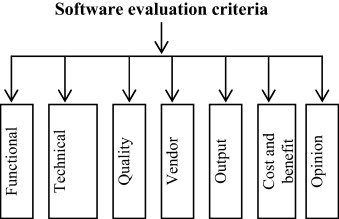
\includegraphics[width=0.5\textwidth]{images/comparision-criteria.jpg}
	\caption{Hauptkriterien des Softwarevergleichs von Jadhav und Sonar \cite{frameworkEvaluation}}
	\label{fig:comparisionCriteria}
\end{figure}
\\
Wie schon Anfangs erwähnt lassen sich nicht alle Kriterien auf Programmiersprachen anwenden, weshalb für diesen konkreten Fall die Kriterien \enquote{Technical} und \enquote{Output} entfallen. Denn mit \enquote{Technical} sind Hardware- und mit \enquote{Output} Ausgabe-Kriterien gemeint, welche in diesem Vergleich keine Anwendung finden.\\
 \\
%Auf Basis des Papers von Jadhav und Sonar wurden die Kriterien, aus der  \hyperref[tab:comparisonCriteria]{Tabelle~\ref{tab:comparisonCriteria}}, für diesen Anwendungsfall ausgearbeitet bzw. angepasst.
 
\subsection{Funktionale Kriterien (Functional)}
\subsubsection{JavaScript-Kompilierung}
\begin{itemize}
	\item In welche JavaScript-Versionen kann kompiliert werden?
	\item Welche Java-Script Modul-System werden unterstützt?
\end{itemize}

\subsubsection{Build-Tools}
\begin{itemize}
	\item Welche Build-Tools werden offiziell unterstützt?
\end{itemize}

\subsubsection{Bibliotheken}
\begin{itemize}
	\item Können schon bestehende JavaScript-Bibliotheken eingebunden werden?
	\item Wie komfortabel ist die Einbindung bestehender Bibliotheken?
	\item Können Java-Bibliotheken eingebunden werden?
\end{itemize}

\subsubsection{Programmierung}
\begin{itemize}
	\item Welcher Programmierstil wird verwendet?
	\item Welcher Grad der Typisierung wird verwendet?
	\item Werden Aspekte der Funktionalen Programmierung unterstützt?
%	\item Wie gut ist die Handhabung Funktionaler Aspekte sofern diese existieren?
\end{itemize}

\subsection{Qualitative Kriterien (Quality)}
\subsubsection{Kommunikationsstandards}
\begin{itemize}
	\item Welche gängigen Formate können standardmäßig verarbeitet werden?
	\item Können diese direkt in Objekte geparst werden?
\end{itemize}

\subsubsection{Browser-Support}
\begin{itemize}
	\item Welche Browser werden unterstützt?
\end{itemize}

\subsubsection{Lernkurve}
\begin{itemize}
	\item Wie leicht lässt sich die Programmiersprache erlernen bzw. bedienen?
	\item Gibt es Online-Plattformen um die Programmiersprache auszuprobieren?
\end{itemize}
 
\subsection{Anwenderkriterien (Vendor)}
\subsubsection{Dokumentation}
\begin{itemize}
	\item Gibt es eine ausführliche Dokumentation?
	\item Gibt es offizielle Tutorials?
\end{itemize}

\subsubsection{Support}
\begin{itemize}
	\item Wird Support von Entwicklern angeboten?
	\item Gibt es ein offizielles Forum oder ähnliches?
	\item Auf welchen weiteren Community-Plattformen ist die Programmiersprache vertreten? 
\end{itemize}

\subsubsection{Community}
\begin{itemize}
	\item Wie viele Entwickler sind an der Programmierung der Sprache beteiligt?
	\item Gibt es Unternehmen welche die Entwicklung unterstützen?
\end{itemize}

\subsection{Kosten- und Nutzenorientierte Kriterien (Cost and benefit)}
\subsubsection{Lizenz}
\begin{itemize}
	\item Wurde die Programmiersprache unter einer freie Lizenz veröffentlicht?
	\item Entstehen durch die Benutzung Lizenzkosten?
\end{itemize}

\subsubsection{Benutzungskosten}
\begin{itemize}
	\item Sind kostenpflichtige Programme für die Benutzung notwendig?
\end{itemize}

\subsection{Kriterien an die öffentliche Meinung (Opinion)}
\subsubsection{Beliebtheit}
\begin{itemize}
	\item Wie viele Repositories gibt es auf Github, welche mit der Programmiersprache entwickelt wurden?
	\item Wie viele Fragen wurden auf der Plattform Stack Overflow zu dieser Programmiersprache gestellt?
\end{itemize}

\subsubsection{Veröffentlichung}
\begin{itemize}
	\item Wann wurde die erste Version veröffentlicht?
\end{itemize}

\subsubsection{Indizies}
\begin{itemize}
	\item Welchen Platz hat die Programmiersprache beim Triobe Index belegt?
	\item Welchen Platz hat die Programmiersprache beim RedMonk Index belegt?
	\item Welchen Platz hat die Programmiersprache beim \gls{PYPL} Index belegt?
\end{itemize}
 
%{
%\small\renewcommand{\arraystretch}{1.4}
%\begin{longtabu} to \textwidth{X[1,L]X[1,L]X[2,L]}
%	\captionabove{Kriterien für den Vergleich zwischen Kotlin und dem Google Web Toolkit in Zusammenhang mit Java} \\
%	\hline
%	\taburowcolors 1{tableheadcolor .. tableheadcolor}
%	\bfseries Hauptkriterium &
%	\bfseries Unterkriterium &
%	\bfseries Leitfragen \\ \hline
%	\endfirsthead
%	\hline
%	Hauptkriterium &
%	Unterkriterium &
%	Leitfragen \\ \hline
%	\endhead
%	\hline
%	\taburowcolors 1{white .. white}
%	\multicolumn{3}{r}{\emph{weiter auf der nächsten Seite \ldots}}
%	\endfoot
%	\hline
%	\endlastfoot
%	\taburowcolors 2{tablebodycolor .. tablerowcolor}
%	Funktional (Functional) 
%		& JavaScript-Kompilierung 
%			& In welche JavaScript-Versionen kann kompiliert werden? \\
%			&& Welche JavaScript Modul-Systeme werden unterstützt? \\
%		& Build-Tools 
%			& Welche Build-Tools werden offiziell unterstützt? \\
%		& Bibliotheken 
%			& Können schon bestehende JavaScript Bibliotheken eingebunden werden? \\
%			&& Wie komfortable ist die Einbindung bestehender Bibliotheken? \\
%			&& Können Java-Bibliotheken eingebunden werden? \\
%		& Programmierung 
%			& Welcher Programmierstil wird verwendet? \\
%			&& Welcher Grad der Typisierung wird verwendet? \\
%			&& Werden Aspekte der Funktionalen Programmierung unterstützt? \\
%			&& Wie gut ist die Handhabung Funktionaler Aspekte sofern diese existieren? \\
%	Qualität (Quality) 
%		& Kommunikationsstandards 
%			& Welche gängigen Formate können standardmäßig verarbeitet werden? \\
%			&& Können diese direkt in Objekte geparst werden? \\
%		& Browser-Support
%			& Welche Browser werden unterstützt? \\
%		& Lernkurve 
%			& Wie leicht lässt sich die Programmiersprache erlernen bzw. bedienen? \\
%			&& Gibt es Online-Plattformen um die Programmiersprache auszuprobieren? \\
%	Anbieter (Vendor) 
%		& Dokumentation 
%			& Gibt es eine ausführliche Dokumentation? \\
%			&& Gibt es offizielle Tutorials? \\
%		& Support
%			& Wird Support von Entwicklern angeboten? \\
%			&& Gibt es ein offizielles Forum oder ähnliches? \\
%			&& Auf welchen weiteren Community-Plattformen ist die Programmiersprache vertreten? \\
%		& Community
%			& Wie viele Entwickler sind an der Programmiersprache beteiligt? \\
%			&& Gibt es Unternehmen welche die Entwicklung unterstützen? \\
%	Kosten und Nutzen (Cost and benefit) 
%		& Lizenz 
%			& Wurde die Programmiersprache unter einer freien Lizenz veröffentlicht? \\
%			&& Entstehen bei der Benutzung Lizenzkosten? \\
%		& Benutzungskosten
%			& Sind kostenpflichtige Programme für die Benutzung notwendig? \\
%	Meinungen (Opinion) 
%		& Beliebtheit 
%			& Wie viele Repositories gibt es auf Github, welche mit der Programmiersprache entwickelt wurden? \\
%			&& Wie viele Fragen wurden auf der Plattform Stackoverflow zu dieser Programmiersprache gestellt? \\
%		& Veröffentlichung
%			& Wann wurde die erste Version veröffentlicht? \\
%		& Tiobe Index
%			& Welchen Platz hat die Programmiersprache belegt? \\
%		& RedMonk Index
%			& Welchen Platz hat die Programmiersprache belegt? \\
%		& PYPL
%			& Welchen Platz hat die Programmiersprache belegt? \\
%\end{longtabu}
%}\label{tab:comparisonCriteria}

\section{Vergleichsergebnis}\label{sec:comparisonResults}

\subsection{Funktionale Kriterien (Functional)}
\subsubsection{JavaScript-Kompilierung}
\begin{description}
	\item[Kotlin] Als Ziel der Kompilierung dient der JavaScript-Standard ECMAScript 5. Es existiert aber bereits Pläne für die Umsetzung des ECMAScript 2015 Standards. Für ein Modul-System kann zwischen \gls{AMD}, CommonJS und \gls{UMD} gewählt werden. \cite{kotlinJavaScript, kotlinJsModules} 
	\item[GWT(Java)] Der Standard ECMAScript 5 dient an dieser stelle ebenfalls als Kompilierungsziel. Auch hier ist bereits eine Planung für den ECMAScript 2015 Support bekannt, welcher mit der Version 3.0 veröffentlicht werden soll. Mittels \gls{GWT} ist es nicht möglich ein JavaScript Modul-System zu verwenden. \cite{gwtRoadmap}
\end{description}

\subsubsection{Build-Tools}
\begin{description}
	\item[Kotlin] Es werden gleich eine ganze Reihe an Build-Tools unterstützt. Vertreten sind dabei Gradle, Maven und Ant, wobei die Nutzung von Gradle für die Kompilierung nach JavaScript offiziell empfohlen wird. \cite{kotlinBuildTools, kotlinToJavaScript}
	\item[GWT(Java)] Nur Ant wird unterstützt, aber auch andere Build-Tools wie zum Beispiel Maven oder Gradle lassen sich über Drittanbieter-Software verwenden. \cite{gwtGettingStarted}
\end{description}

\subsubsection{Bibliotheken}
\begin{description}
	\item[Kotlin] Es besteht die Möglichkeit bereits erstellte JavaScript-Bibliotheken, mittels \gls{JsInterop} zu integrieren. Dafür muss die \gls{API} der Bibliothek nachgebaut werden. Da das für große Projekte sehr mühselig sein kann, biete Kotlin dafür das Tool \enquote{ts2kt}\footnote{siehe \url{https://github.com/Kotlin/ts2kt}} an, welches diese Aufgabe übernimmt. Voraussetzung dafür ist nur die Existenz der zugehörigen TypeScript Definitionsdateien. Eine Integration von Java-Bibliotheken ist nicht möglich. \cite{kotlinJsInteop, kotlinJsJavaToJs}
	\item[GWT(Java)] Ebenso wie in Kotlin besteht die Möglichkeit der Einbindung bereits bestehender JavaScript-Bibliotheken, mithilfe von \gls{JsInterop} oder \gls{JSNI}. Aber es wird jedoch nicht mehr empfohlen  \gls{JSNI} zu benutzen, weil diese Technologie veraltet ist und mit der Version 3.0 entfernt wird. Im Gegensatz zu Kotlin können in \gls{GWT} auch Java-Bibliotheken eingebunden, was daher geschuldet ist das generell Java-Code in JavaScript-Code kompiliert wird. \cite{gwtJsInterop, gwtJSNI}
\end{description}

\subsubsection{Programmierung}
\begin{description}
	\item[Kotlin] Kotlin ist eine statisch typisierte objekt-orientierte Programmiersprache, welche ebenso Aspekte der Funktionalen Programmierung enthält. \cite{kotlinInfo}
	\item[GWT(Java)] Auch wie Kotlin ist Java eine statisch typisierte objekt-orientierte Programmiersprache. Funktionale Aspekte wie beispielsweise Lambda-Ausdrücke wurde mit der Version 8 ergänzt. \cite{java8Specification}
\end{description}

\subsection{Qualitative Kriterien (Quality)}
\subsubsection{Kommunikationsstandards}
\begin{description}
	\item[Kotlin] Mithilfe der Bibliothek \enquote{kotlinx.serialization} können die Formate \gls{JSON}, \gls{CBOR} und Protobuf verarbeitet und auch direkt in Objekte geparst werden. Dabei besteht auch die Möglichkeit die Bibliothek für weitere Formate zu erweitern. Das Format \gls{XML} kann auch mit Standard JavaScript Methoden verarbeitet, aber nicht direkt in Objekte geparst werden. \cite{kotlinxSerialization}
	\item[GWT(Java)] Auch \gls{GWT} bietet die Möglichkeit \gls{JSON} in Objekte zu parsen, aber genau wie bei Kotlin gilt das nicht für das Format \gls{XML}. Hierfür werden zwar benötigte Funktionen und Methoden durch \gls{GWT} bereitgestellt, aber ein Objekt-Parsing ist dennoch nicht möglich. Andere Formate werden nicht offiziell unterstützt. \cite{gwtJSON, gwtXML}
\end{description}

\subsubsection{Browser-Support}
\begin{description}
	\item[Kotlin] Offiziell gibt es keine Information welche Browser unterstützt werden.
	\item[GWT(Java)] Die Browser Internet Explorer in den Versionen acht, neun, zehn und elf, Safari in den Versionen fünf und sechs, Firefox, Chrome und Opera werden offiziell unterstützt. \cite{gwtGettingStarted}
\end{description}

\subsubsection{Lernkurve}
\begin{description}
	\item[Kotlin] Es wird eine kompakte Einführung bereitgestellt, welche auf ein schnelles erfolgreiches Ergebnis abzielt. Des weiteren gibt es eine ganze Reihe an Tutorials, welche sehr ausführlich erläutert und immer mit reichlich Beispielen bestückt sind. Zu dem wird außerdem noch eine Online-Plattform\footnote{siehe \url{https://try.kotlinlang.org/}} angeboten, wo weitere Beispiele direkt ausgeführt und auch eigener Code getestet werden kann. \cite{kotlinReference}
	\item[GWT(Java)] Auch für die Bibliothek \gls{GWT} wird eine Kompakte Einführung mit schnellem Ergebnis bereit gestellt. Ergänzend dazu gibt es eine ganze Reihe an Tutorials, wo auch etwas größere und komplexere Beispiele vertreten sind. Leider gibt es für \gls{GWT} keine Online-Plattform, um ohne eine Installation diese zu testen, aber für Java\footnote{\url{https://www.jdoodle.com/online-java-compiler}} gibt es solche. \cite{gwtGettingStarted}
\end{description}


\subsection{Anwenderkriterien (Vendor)}
\subsubsection{Dokumentation}
\begin{description}
	\item[Kotlin] Die Dokumentation von Kotlin ist sehr ausführlich und verständlich erläutert. Dabei wird diese, wie schon zuvor erwähnt, durch eine ganze Reihe an Tutorials unterstützt. \cite{kotlinReference}
	\item[GWT(Java)] Für \gls{GWT} und auch für Java gibt es eine sehr ausführliche, mit Tutorials bestickte Dokumentation. \cite{gwtDevGuide, javaDoc}
\end{description}

\subsubsection{Support}
\begin{description}
	\item[Kotlin] Durch die Firma JetBrains, welche für die Entwicklung von Kotlin verantwortlich ist, wird kein offizieller Support angeboten. Fragen können in dem offiziellen Forum\footnote{siehe \url{https://discuss.kotlinlang.org/}} gestellt werden, wo auch jede Menge offizielle Entwickler vertreten sind und auch auf die Fragen eingehen. Zusätzlich können Informationen oder auch Fragen auf den Community-Plattformen Reddit, Slack, Stack Overflow, Twitter oder Google+ erhalten bzw. gestellt werden. \cite{kotlinCommunity}
	\item[GWT(Java)] Genau wie Kotlin bietet \gls{GWT} eine ganze Reihe von Community-Plattformen an. Darunter Reddit, Stack Overflow, Twitter und Google+. Als Forum dienen verschiedene je nach Anwendungsfall spezialisierte Google Gruppen. \cite{gwtCommunity}
\end{description}

\subsubsection{Community}
\begin{description}
	\item[Kotlin] Laut dem Repository auf Github haben sich bisher 233(Stand 13.06.2018) Leute beteiligt. Davon sind laut eigenen Aussagen über 40 Teilnehmer von JetBrains gestellt. \cite{kotlinWhoDevelops}
	\item[GWT(Java)] Für Java existiert keine konkrete Zahl an beteiligten Entwicklern, bekannt ist nur das die Community von den großen Firmen Oracle und IBM unterstützt wird. \gls{GWT} hat laut Github 87 Beteiligte und wird von der Firma Google entwickelt bzw. unterstützt. \cite{oracleIBMCollaborate, gwtTerms}
\end{description}


\subsection{Kosten- und Nutzenorientierte Kriterien (Cost and benefit)}
\subsubsection{Lizenz}
\begin{description}
	\item[Kotlin] Diese Projekt wurde unter der freien Apache-Lizenz in der zweiten Version verwendet. Daher entstehen bei der Benutzung der Programmiersprache keinerlei Kosten. \cite{kotlinFree}
	\item[GWT(Java)] Auch Java und \gls{GWT} lassen sich kostenlos nutzen, denn diese werden ebenfalls unter freien Lizenzen veröffentlicht. Im Falle von Java ist das die \gls{GPL} mit Classpath Exception und bei \gls{GWT}, genau wie bei Kotlin, die Apache-Lizenz in der zweiten Version. \cite{javaLicense, gwtTerms}
\end{description}

\subsubsection{Benutzungskosten}
\begin{description}
	\item[Kotlin] Um mit Kotlin ein Projekt zu starten ist keinerlei kostenpflichtiges Programm notwendig. Zum entwickeln können die Plugins für die kostenlosen \glspl{IDE} IntelliJ IDEA, Android Studio oder Eclipse benutzt werden. Alternativ steht auch ein \enquote{standalone} Compiler zur Verfügung.
	\item[GWT(Java)] Auch für Java- bzw. \gls{GWT}-Projekte fallen keine Kosten an. Die Auswahl an \glspl{IDE} ist noch etwas größer als bei Kotlin. Unter anderem sind dabei IntelliJ IDEA, Eclipse und NetBeans IDE vertreten. Bei der Installation des \gls{SDK} von Java wird zwar ein Compiler mitgeliefert, aber um ein \gls{GWT}-Projekt zu kompilieren muss das Build Tool Ant benutzt werden, welches aber ebenfalls kostenlos zur Verfügung steht.
\end{description}


\subsection{Kriterien an die öffentliche Meinung (Opinion)}
\subsubsection{Beliebtheit}
\begin{description}
	\item[Kotlin] Laut Github existieren derzeit über 72~590\footnote{siehe \url{https://api.github.com/search/repositories?q=language:Kotlin}} Repositories, welche mit Kotlin entwickelt wurden bzw. noch werden. Die Zahl der auf Stack Overflow gestellten Fragen beläuft sich auf 11~398\footnote{siehe \url{https://stackoverflow.com/questions/tagged/kotlin}}. (Stand: 14.06.2018)
	\item[GWT(Java)] Die Anzahl der Github-Repositories beträgt derzeit 4~810~228\footnote{siehe \url{https://api.github.com/search/repositories?q=language:Java}} für Java-Projekte. Da \gls{GWT} ein Framework ist lässt es sich über Github nicht ermitteln wie viele Repositories dieses benutzen. Bei den Fragen auf Stack Overflow sieht das anders aus, denn derzeit sind 1~426~726\footnote{siehe \url{https://stackoverflow.com/questions/tagged/java}} mit Java und 20~443\footnote{siehe \url{https://stackoverflow.com/questions/tagged/gwt}} mit \gls{GWT} getaggt. (Stand: 14.06.2018)
\end{description}

\subsubsection{Veröffentlichung}
\begin{description}
	\item[Kotlin] Am 22. Juli 2011 wurde Kotlin erstmals als neue Sprache für die \gls{JVM} vorgestellt und am 15. Februar 2016 wurde die erste Version released. \cite{kotlinNewForJVM, kotlinRelease}
	\item[GWT(Java)] Die erste Version von Java wurde 23. Mai 1995 und die von \gls{GWT} am 16. Mai 2006 veröffentlicht. \cite{javaRelease, gwtRelease}
\end{description}

\subsubsection{Indizies}
\begin{description}
	\item[Kotlin] Laut Tiobe Index landet Kotlin im Ranking der beliebtesten Programmiersprache auf Platz 49, laut RedMonk Index auf Platz 27 und laut PYPL Index auf Platz 16. \cite{tiobeIndex, redMonkIndex, pyplIndex}
	\item[GWT(Java)] Da \gls{GWT} keine Programmiersprache ist beziehen sich die Platzierungen nur auf Java, welche laut Tiobe Index den Platz eins und laut RedMonk und PYPL Index den Platz zwei belegt. \cite{tiobeIndex, redMonkIndex, pyplIndex}
\end{description}


%\begin{longtabu} to \textwidth {X[L]X[L]X[L]}
%	\captionabove{Vergleichsergebnis zwischen Kotlin und dem Google Web Toolkit in Zusammenhang mit Java} \\
%	\hline
%	\taburowcolors 1{tableheadcolor .. tableheadcolor}
%	\bfseries Leitfrage &
%	\bfseries Kotlin &
%	\bfseries Google Web Toolkit/Java\\ \hline
%	\endfirsthead
%	\hline
%	Leitfrage &
%	Kotlin &
%	Google Web Toolkit/Java\\ \hline
%	\endhead
%	\hline
%	\taburowcolors 1{white .. white}
%	\multicolumn{3}{r}{\emph{weiter auf der nächsten Seite \ldots}}
%	\endfoot
%	\hline
%	\endlastfoot
%	\taburowcolors 2{tablebodycolor .. tablerowcolor}
%	L-1.1 
%		& ECMAScript 5 (ECMAScript 2015 Support ist in Bearbeitung) \cite{kotlinJavaScript}
%			& ECMAScript 5\\
%\end{longtabu}
% !TeX encoding=utf8
% !TeX spellcheck = de_DE
% !TeX root = ../Diploma.tex

\chapter{Konzept des Servers}
Inhalt dieses Kapitels soll die Planung sein, welche für die Umsetzung des RESTful Schachservers benötigt wird. Dabei dient der erste Abschnitt für eine Erläuterung der Anforderungen, welche der Server mitbringen bzw. erfüllen soll. Enthalten ist dabei auch eine Erläuterung der benötigten Ressource. Im zweiten Abschnitt dieses Kapitels befasst sich anschließend damit, wie der Zugriff auf einzelne Ressourcen des REST-Server erfolgen soll. Dabei werden alle möglichen Request-Methoden für die jeweiligen Ressourcen näher beleuchtet.

\section{Anforderungen}\label{sec:anforderungen}
Die Grundanforderungen an den RESTful Schachserver sollen in erster Linie die Bereitstellung aller benötigten Ressourcen sein. Dabei sollen Elemente erstellt, ggf. bearbeitet und gelöscht werden können. Zusätzlich soll die Möglichkeit bestehen, einzelne oder alle gespeicherten Elemente einer Ressource abzufragen. Beim erstellen eines neuen Ressourcenelements soll dieses in einer SQLite Datenbank gespeichert und die ID automatisch durch SQLite generiert werden.\\
\\
Um ein Schachspiel abzubilden bedarf es dabei der Ressourcen Player (Spieler), Match (Partie) und Draw (Zug), welche in den nachfolgenden \hyperref[sec:resplayer, sec:resdraw]{Unterabschnitten~\ref{sec:resplayer} bis \ref{sec:resdraw}} näher betrachtet werden.\\
\\
Als abschließende Anforderung ist noch die Fehlerresistenz zu erwähnen. Denn die im Rahmen dieser Arbeit entstandene Praktikumsaufgabe \todo[inline]{Verweis auf Praktikumsaufgabe im Anhang} soll durch zukünftige Studenten absolviert werden, wobei der Server als Grundlage dienen soll.\\
\\
Zur Unterstützung der Erläuterungen in den \hyperref[sec:resplayer, sec:resdraw]{Kapiteln~\ref{sec:resplayer} bis \ref{sec:resdraw}} bietet die \hyperref[fig:classdiagram]{Abbildung~\ref{fig:classdiagram}}, in Form eines \gls{UML} Klassendiagramms, eine Veranschaulichung.
\begin{sidewaysfigure}
	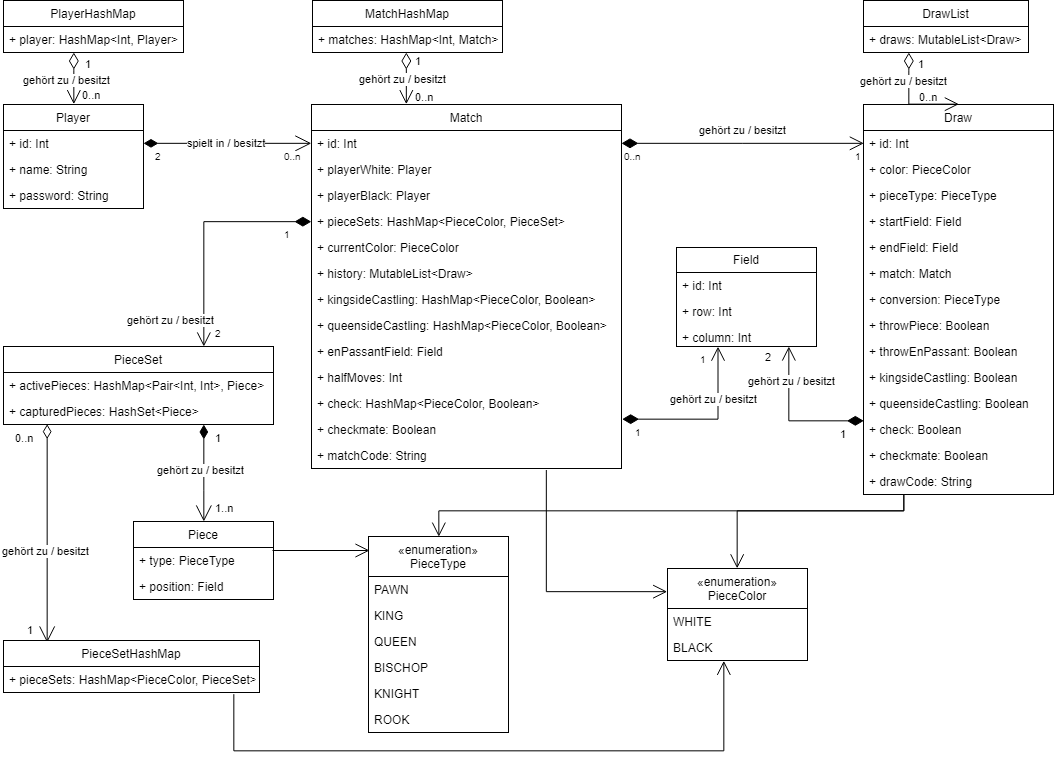
\includegraphics[width=0.9\textwidth]{images/classdiagram.png}
	\caption{Klassendiagramm: Modelle des Servers}
	\label{fig:classdiagram}
\end{sidewaysfigure}

\subsection{Ressource: Player (Spieler)}\label{sec:resplayer}
Neben der ID, welche schon im Abschnitt \ref{sec:anforderungen} erwähnt und durch die SQLite Datenbank generiert werden soll, besitzt der Player noch Informationen über seinen Name und sein Passwort.\\
\\
Nach dem anlegen eines neuen Players soll eine Änderung des Namens nicht gestattet sein, die des Passwortes hingegen schon.

\subsection{Ressource: Match (Partie)}\label{sec:resmatch}
Neben der ID besitzt ein Match Informationen über die beiden Spielteilnehmer und deren Figurenstellung auf dem Schachbrett. Zusätzlich wird registriert welcher der beiden Player als nächstes seinen nächsten Zug tätigen muss, welche Möglichkeiten zum rochieren bestehen, ob ein Schlag \enquote{en passant} möglich ist und wenn ja auf welches Feld gezogen werden muss und wie viele Halbzüge gespielt wurden. Der Wert der Halbzüge wird zurückgesetzt sobald eine Bauernfigur gezogen oder eine beliebige Figur geschmissen wurde. Zusätzlich kann über ein Match ermittelt werden ob ein Spieler im Schach steht oder ob das Spiel schon bis zum Schachmatt gespielt wurde. All diese Informationen werden zusätzlich noch als String in der \gls{FEN}\footnote{\label{foot:chapter}siehe Kapitel 2.3} gespeichert.

\subsection{Ressource: Draw (Zug)}\label{sec:resdraw}
Die Ressource Draw speichert zusätzlich zur ID die Farbe des Spielers, die Art der Spielfigur, Start- und Endfeld des Zuges, ob eine Figur geschlagen wurde, wenn ja ob durch en passant und ob seitens der Dame oder des König rochiert wurde. Die Informationen werden ähnlich zum Match als String gespeichert, aber in diesem Fall in der \gls{SAN}\footref{foot:chapter}.

\section{Ressourcenzugriffe mithilfe von Controllern}
Die einzelnen Zugriffe auf die Ressourcen werden in den \hyperref[sec:playerController, sec:drawController]{Kapiteln~\ref{sec:playerController} bis \ref{sec:drawController}} nach ihrer Art bzw. deren Aufgaben in einzelne Controller unterteilt, um eine gute Übersicht zu wahren. Für alle Einstiegspunkte der \gls{REST}-\gls{API} soll die Request-Methode \enquote{OPTIONS} bereitstehen, über welchen ermittelt werden kann welche Methoden für den jeweiligen Einstiegspunkt zur Verfügung stehen.\\
\\
Etwaige Requestparameter sollen in dem Format \gls{JSON} oder x-www-form-urlencode mitgeschickt werden können. Die gesendeten Anfragen sollen ihr Feedback je nach Wunsch, via Content Negotiation, entweder in \gls{JSON} oder in \gls{XML} zurücksenden. Dabei sollen drei Strategien bereitgestellt werden, entweder mittels Suffix, einem URL-Parameter oder dem \gls{HTTP} Accept-Header. 

\subsection{Player Controller}\label{sec:playerController}
Der Player Controller soll zwei Einstiegspunkt an den \glspl{URI} \code{/player/} und \code{/player/\{id\}} zur Verfügung stellen. Der Parameter \code{\{id\}} dient dabei als Platzhalter für die ID eines Players, welche wiederum als Zahl dargestellt wird.\\
\\
Am ersten Einstiegspunkt soll eine Liste aller Spieler über einen GET-Request bereitgestellt werden können. Des weiteren soll an diesem die Möglichkeit bestehen einen neuen Player mithilfe eines POST-Requests zu erzeugen. Dabei muss als Parameter der Name und das Passwort des Players mitgegeben werden. Die SQLite-Datenbank soll die ID dabei automatisch mittels Autoincrement erzeugen. Bei erfolgreicher Erstellung des Players soll dieser zurückgegeben werden, ansonsten \code{NULL}.\\
\\
Am zweiten Einstiegspunkt soll ein einzelner existierender Player über einen GET-Request bereitgestellt, über einen DELETE-Request gelöscht und über einen PATCH-Request aktualisiert werden können. Nur das Passwort darf dabei laut Anforderungen\footnote{siehe \hyperref[sec:anforderungen]{Kapitel~\ref{sec:anforderungen}}} aktualisiert werden, wobei dieses zusätzlich als Parameter an den Request mit angehangen werden muss.\\
\\
Für ein besseres Verständnis bietet die \hyperref[fig:playerController]{Abbildung~\ref{fig:playerController}} eine visuelle Verdeutlichung der Einstiegspunkte des Player Controllers.
\begin{figure}[htb]
	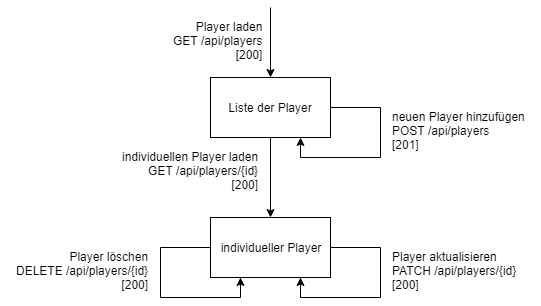
\includegraphics[width=0.7\textwidth]{images/player-controller.png}
	\caption{Player Controller - Übersicht der Einstiegspunkte}
	\label{fig:playerController}
\end{figure}

\subsection{Match Controller}\label{sec:matchController}
Die \glspl{URI} \code{/match/}, \code{/match/\{id\}}, \code{/match/{id}/draws} und \code{/match/{id}/pieceSets} sollen durch den Match Controller bereitgestellt werden.\\
\\
Dabei soll die erste \gls{URI} ebenso wie beim \enquote{Player Controller} Zurverfügungstellung einer Liste aller registrierten Matches und dem anlegen neuer dienen. Das Bereitstellen der Liste soll mittels GET- und das anlegen mittels POST-Request erfolgen. Der GET-Request soll zwei optionale boolesche Parameter bereitstellen, womit das Senden der Historie von Draws bzw. der Figurenstellung bestimmt werden soll. Standardmäßig sollen dabei die Parameter \code{TRUE} sein. Weiter unten in diesem Kapitel wird beschrieben wie diese Informationen separat geholt werden können. Um ein neues Match zu registrieren, müssen dabei die ID's der beiden Spielteilnehmer mitgeschickt werden. Anhand des Parameternamens soll festgelegt werden welcher Spieler Weiß und welcher Schwarz spielen soll.\\
\\
Der zweite Einstiegspunkt soll in diesem Controller ausschließlich dazu verwendet werden, um einzelne Matches mithilfe eines GET-Request anzufordern oder mithilfe eines DELETE-Request zu löschen. Für das anfordern eines einzelnen Matches stehen ebenso zwei boolesche, wie beim Anfordern einer Liste, bereit. Wenn ein Nutzer ein Match löscht, sollen ebenfalls alle zugehörigen Draws gelöscht werden. Um eine unrechtmäßige Manipulation der Match-Daten durch einen Nutzer zu verhindern, soll keine Möglichkeit bereitstehen ein Match zu aktualisieren. Die Aktualisierung eines Matches soll ausschließlich durch das hinzufügen von Draws erfolgen.\footnote{siehe \hyperref[sec:drawController]{Kapitel~\ref{sec:drawController}}}\\
\\
Die letzten beiden Einstiegspunkte sollen dazu dienen große Match bezogene Daten separat zu ermitteln. Dabei soll mittels GET-Request an der \gls{URI} \code{/match/{id}/draw} eine Liste aller Draws und über die \gls{URI} \code{/match/{id}/pieceSets} eine Map mit allen Figuren der beiden Spielteilnehmer bereitgestellt werden. Neben den aktuell auf dem Spielfeld stehenden Figuren sollen dabei auch die geschmissen mitgeschickt werden.\\
\\
Die \hyperref[fig:matchController]{Abbildung~\ref{fig:matchController}} bietet für die zuvor definierten Einstiegspunkte eine grafische Veranschaulichung.
\begin{figure}[htb]
	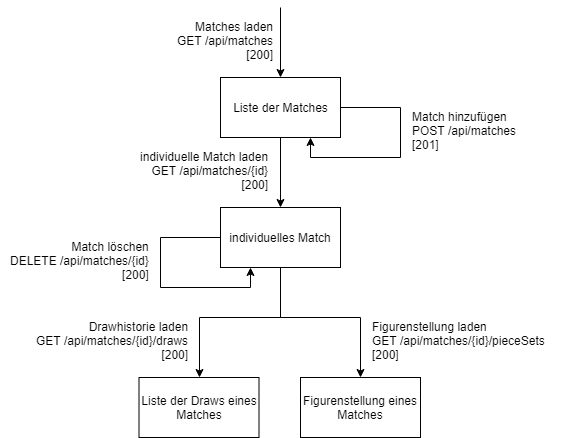
\includegraphics[width=0.7\textwidth]{images/match-controller.png}
	\caption{Match Controller - Übersicht der Einstiegspunkte}
	\label{fig:matchController}
\end{figure}

\subsection{Draw Controller}\label{sec:drawController}
Auch der Draw Controller stellt wieder zwei Einstiegspunkte an den \glspl{URI} \code{/draw/} und \code{/draw/\{id\}} bereit. \\
\\
Am ersten Einstiegspunkt soll wieder das bereitstellen einer Liste mittels GET- und das hinzufügen mittels POST-Request von Draws zur Verfügung gestellt werden. Für das hinzufügen eines neuen Draws ist die ID des Matches und der Draw-Code in der \gls{SAN} als Parameter von nöten. Zusätzlich soll die Möglichkeit bestehen die Zeilen- und die Spaltennummer der Startposition mitzugeben. Wenn diese Informationen nicht mitgegeben werden, so soll der Controller die Startposition kalkulieren. Spalten sollen dabei als Nummern und nicht als Buchstaben mitgegeben werden\footnote{A $\rightarrow$ 8; ...; H $\rightarrow$ 8}. Nach erfolgreicher Validierung des Draw-Codes soll der Draw dem zugehörigen Match hinzugefügt und die Match-Daten aktualisiert werden.\\
\\
Über den zweiten Einstiegspunkt soll wieder die Abfrage nach einem einzelnen Draw möglich sein. Eine Möglichkeit zum Löschen oder Aktualisieren des Draws soll nicht bestehen, da sonst der Nutzer wieder eine Möglichkeit hätte das Match zu manipulieren. Das Löschen von Draws soll über die Löschung des dazugehörigen Matches erfolgen\footnote{siehe \hyperref[sec:matchController]{Kapitel~\ref{sec:matchController}}}.\\
\\
Wie in den vorherigen Kapiteln bietet die \hyperref[fig:drawController]{Abbildung~\ref{fig:drawController}} ein Veranschaulichung.
\begin{figure}[htb]
	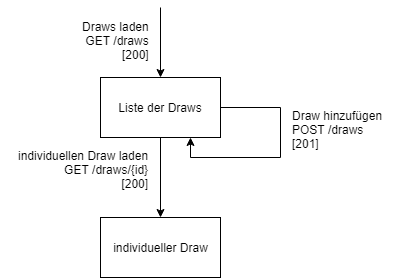
\includegraphics[width=0.54\textwidth]{images/draw-controller.png}
	\caption{Draw Controller - Übersicht der Einstiegspunkte}
	\label{fig:drawController}
\end{figure}
% !TeX encoding=utf8
% !TeX spellcheck = de_DE
% !TeX root = ../Diploma.tex

\chapter{Konzept des Clients}\label{sec:conceptClient}
In diesem Kapitel soll die Planung des Schachclients näher erläutert werden, welches als Grundbaustein für die Implementierung dienen soll. Dabei dient der erste Abschnitt zur Beschreibung der benötigten Anforderung, welche der Client erfüllen soll. Der zweiten Abschnitt sollen der Visualisierung und Beschreibung der einzelnen Ansichten dienen, welche für eine bequeme Nutzerinteraktion benötigt werden.

\section{Anforderungen}\label{sec:anforderungenClient}
Grundlegen soll der Client als Visualisierung des Servers dienen. Dafür soll dieser eine Verwaltung von Playern und Matches bereitstellen, inklusive der Möglichkeit zum Anlegen neuer bzw. bearbeiten schon angelegter Einträge. Um anschließend auch Schach spielen zu können muss der Client dafür eine komfortable Möglichkeit, in Form eines virtuellen Schachbrettes, bieten.\\
\\
Als Grundanforderung dafür muss der Client natürlich mit dem Server kommunizieren können. Dafür muss dieser Requests senden und die empfangenen Response-Nachrichten verarbeiten können. Da der Server für manche Request spezielle Parameter benötigt, wie zum Beispiel einen String in der \gls{SAN}, müssen diese gegebenenfalls ermittelt werden können.\\
\\
Für ein bequemes Spielerlebnis soll der Client ein gestartetes Match automatisch aktualisieren, sobald sich die Daten auf dem Server verändert haben. Um dies zu realisieren soll ein einfaches Polling-Verfahren implementiert werden.\\
\\ 
Die letzte Grundanforderung soll eine innovative und benutzerfreundliche Bedienung der Anwendung sein, so das der Nutzer keinerlei Kenntnisse, bis auf die Schachregeln, besitzen muss.

\section{Mockup-Entwicklung der benötigten Client-Ansichten}\label{sec:views}
In diesem Abschnitt sollen die im \hyperref[sec:anforderungenClient]{Kapitel~\ref{sec:anforderungenClient}} zuvor definierten Anforderungen konkretisiert und visuell aufbereitet werden. Ziel soll dabei die Erstellung von Mockups der einzelnen Ansichten sein, um die Implementierung zu vereinfachen bzw. zu beschleunigen.

\subsection{Startansicht}\label{sec:startView}
Diese Ansicht soll als Ausgangspunkt für die Nutzer dienen. Sie sollen zurückgegeben werden, sobald die Root-\gls{URL} aufgerufen wurde. Mithilfe der Startansicht soll dem Nutzer die Möglichkeit bereitgestellt werden zur Player-Ansicht bzw. zur Match-Ansicht zu wechseln. Dafür soll ihm jeweils ein Button zum Auslösen dieses Wechsels zur Verfügung gestellt werden.\\
\\
Die \hyperref[fig:startView]{Abbildung~\ref{fig:startView}} visualisiert dabei die zuvor definierten Anforderungen an die Startansicht.
\begin{figure}[htb]
	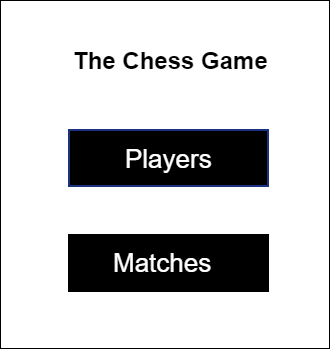
\includegraphics[width=0.9\textwidth]{images/start-view.png}
	\caption{Mockup: Startansicht des Clients}
	\label{fig:startView}
\end{figure}

\subsection{Player-Ansicht}\label{sec:playerView}
Mit dieser Ansicht soll der Nutzer die Möglichkeit erhalten alle angelegten Player zu verwalten. Dafür soll ihm eine Tabelle für die Übersicht und ein Formular zum anlegen neuer oder bearbeiten bereits angelegter Player bereitgestellt werden. Über eine Spalte innerhalb der Tabelle sollen Buttons zur Verfügung stehen, über welche ein Player bearbeitet oder gelöscht werden kann.\\
\\
Aus diesen gegebenen Anforderungen wurde das Mockup aus der \hyperref[fig:playerView]{Abbildung~\ref{fig:playerView}} entworfen, um diese visuell hervorzuheben.
\begin{figure}[htb]
	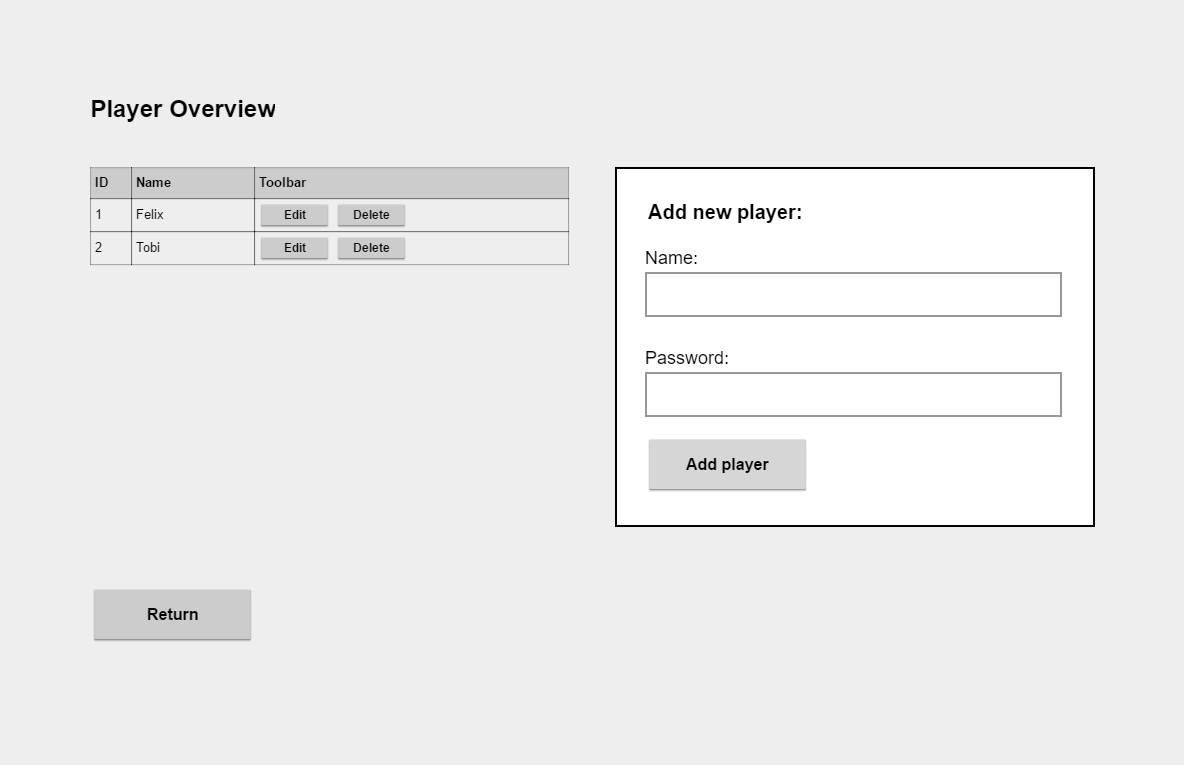
\includegraphics[width=0.9\textwidth]{images/player-view.png}
	\caption{Mockup: Player-Ansicht des Clients}
	\label{fig:playerView}
\end{figure}

\subsection{Match-Ansicht}\label{sec:matchView}
Mithilfe der Match-Ansicht soll dem Nutzer eine Ansicht zur Match-Verwaltung zur Verfügung stehen. Um dabei die Konsistenz zu wahren ist auch diese genau so aufgebaut wie die Player-Ansicht. Mit dem Unterschied das ein Match nicht gelöscht aber dafür gestartet werden kann. Daher ändern sich geringfügig die Buttons in der Tabelle.\\
\\
Dabei werden die Anforderungen durch die \hyperref[fig:matchView]{Abbildung~\ref{fig:matchView}} grafisch dargestellt.
\begin{figure}[htb]
	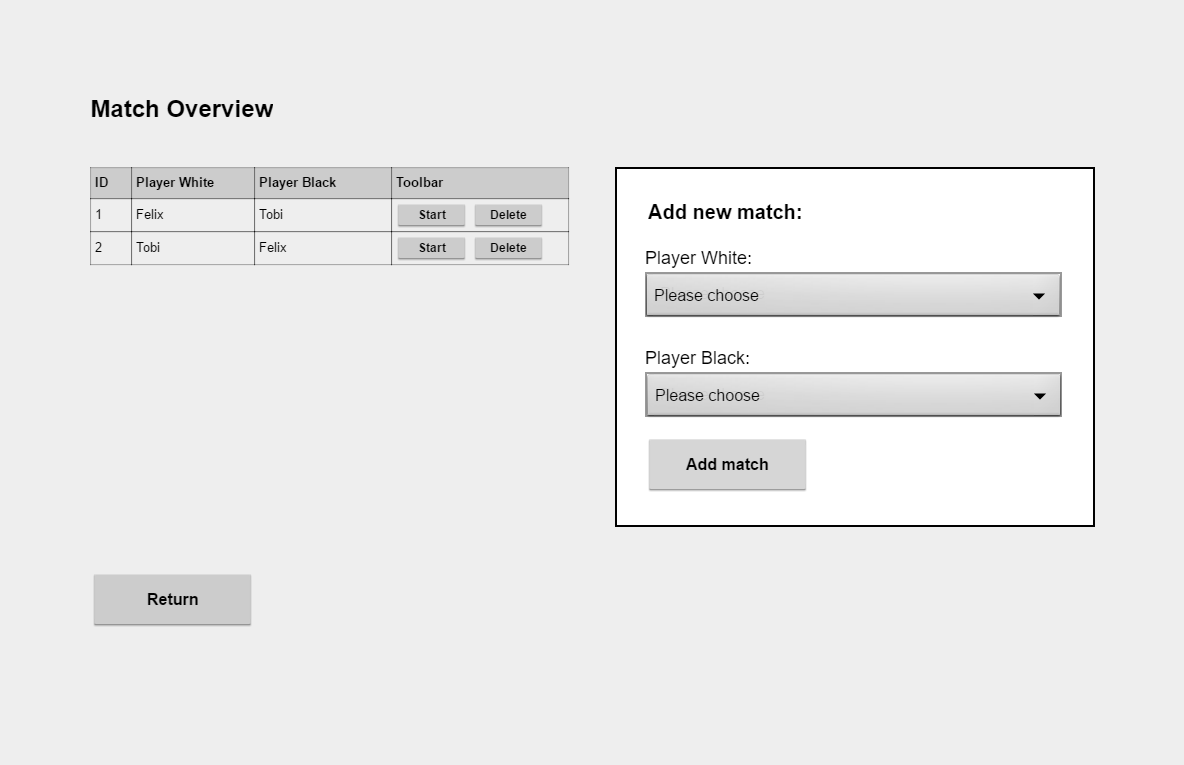
\includegraphics[width=0.9\textwidth]{images/match-view.png}
	\caption{Mockup: Match-Ansicht des Clients}
	\label{fig:matchView}
\end{figure}

\subsection{Ansicht eines gestarteten Matches}\label{sec:gameView}
Mithilfe dieser Ansicht soll dem Nutzer ermöglicht werden ein gestartetes Match zu spielen. Dafür wird in erster Linie ein Schachbrett benötigt, auf welchem die Figuren dargestellt werden. Mittels \enquote{Drag \& Drop} soll der Nutzer anschließend Spielfiguren bewegen können. Für eine einfachere Bedienung und zur Unterstützung des Verständnisses der Schachregeln, sollen alle möglichen Züge einer Figur hervorgehoben werden, sobald über diese mit der Maus gefahren wird. Da Informationen über bereits geschmissene Figuren oder welche Züge bisher getätigt wurden sehr hilfreich sein können, sollen diese neben dem Schachbrett dargestellt werden. \\
\\
Anhand dieser Kriterien an die Ansicht eines gestarteten Matches wurde das Mockup aus der \hyperref[fig:gameView]{Abbildung~\ref{fig:gameView}} entwickelt.
\begin{figure}[htb]
	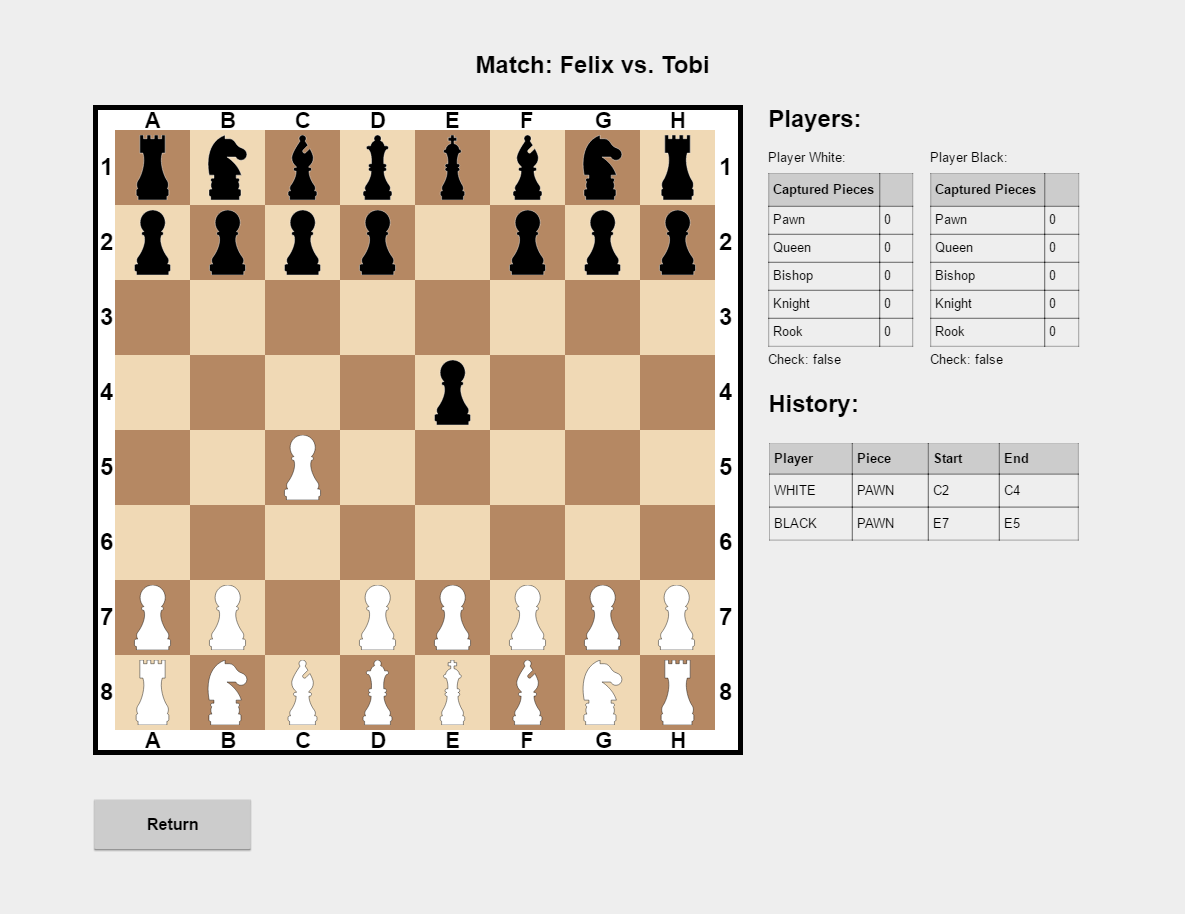
\includegraphics[width=0.9\textwidth]{images/game-view.png}
	\caption{Mockup: Ansicht eines gestarteten Matches}
	\label{fig:gameView}
\end{figure}



% !TeX encoding=utf8
% !TeX spellcheck = de_DE
% !TeX root = ../Diploma.tex

\chapter{Implementation des Servers}
Inhalt dieses Kapitels soll die Umsetzung des Konzeptes aus \hyperref[sec:conceptServer]{Kapitel~\ref{sec:conceptServer}} sein. Dafür wird im ersten Abschnitt auf die Bibliotheken bzw. Frameworks eingegangen, welche für die Umsetzung verwendet wurden. Der zweite Teil wird die Anbindung zur Datenbank näher betrachtet. Anschließend folgt eine Erläuterung zur Konfiguration von Content-Negotiation einer Spring-Applikation. In dem vierten Unterkapitel wird die Fehlerbehandlung bzw. das Exceptionhandling näher erläutert. Der letzte Abschnitt befasst sich mit der Ermittlung bzw. Analyse der Schachnotationen \gls{FEN} und \gls{SAN}.

\section{Verwendete Bibliotheken/Frameworks}
Die verwendeten Bibliotheken bzw. Frameworks sollen die Umsetzung der Anforderungen aus dem \hyperref[sec:anforderungen]{Kapitel~\ref{sec:anforderungen}} vereinfachen und beschleunigen. Dabei werden diese in den nachfolgenden \hyperref[sec:bibspring, sec:bibfasterxml]{Unterabschnitten~\ref{sec:bibspring} bis \ref{sec:bibfasterxml}} in den Punkten Zweck, Einrichtung und Verwendung näher betrachtet. 

\subsection{Spring}\label{sec:bibspring}
Spring wird als ein leichtgewichtiges Framework für die Umsetzung von Java Applikationen beschrieben. Dabei bezieht sich das leichtgewichtig nicht auf die Größe oder Anzahl der enthaltenen Klassen. Es ist eher als geringer Aufwand an Änderungen am eigenen Programmcode zu verstehen, um die Vorteile des Frameworks nutzen zu können. \cite{proSpring5} Spring biete eine Vielzahl an Einsatzmöglichkeiten, aber für die Umsetzung des Servers soll es für die Erzeugung der \gls{REST}-\gls{API} dienen.\\
\\
Um Spring in einem Projekt einzubinden, müssen die Zeilen aus dem \hyperref[lst:includeSpring]{Listing~\ref{lst:includeSpring}}, zusätzlich zu denen welche Kotlin benötigt\todo{ggf. irgendwo beschreiben wie man Kotlin in Gradle einbindet}, in der Build-Datei \enquote{build.gradle} eingefügt werden.
\begin{lstlisting}[style=lstStyleFramed, language=Gradle, caption={Einbindung des Spring Framework mithilfe von Gradle}, label=lst:includeSpring, float]
buildscript {
	repositories {
		mavenCentral()
	}
	dependencies {
		classpath "org.jetbrains.kotlin:kotlin-allopen:1.2.30"
		classpath "org.springframework.boot:spring-boot-gradle-plugin:1.5.4.RELEASE"
	}
}
apply plugin: "kotlin-spring"
apply plugin: "org.springframework.boot"

repositories {
	mavenCentral()
}

dependencies {
	compile "org.springframework.boot:spring-boot-starter-web"
}
\end{lstlisting}
Zu beachten ist dabei das Gradle nur eine Lösung für die Einbindung ist. Da aber für die Umsetzung ebenfalls Gradle verwendet wird, werden alle anderen Lösungen an dieser Stelle vernachlässigt.\\
\\ 
Für die Erstellung einer \gls{REST} \gls{API} muss zunächst ein Controller für eine Ressource angelegt werden, dabei ist es sinnvoll für jede einen eigenen Controller zu definieren. Innerhalb werden anschließend alle Einstiegspunkte erzeugt. Als Beispiel soll das \hyperref[lst:springcontroller]{Listing~\ref{lst:springcontroller}} in Form eines klassischen \code{Hello World} dienen. Dafür wird eine Klasse \code{GreetingController} mit einer Funktion \code{getGreeting} definiert. Als Parameter bekommt diese Funktion einen Namen übergeben, welcher standardmäßig den String \code{World} hält. An dieser Stelle kommt das Spring Framework ins Spiel. Dieses stellt eine Reihe von Annotation bereit, wobei \code{@RestController} einen Controller für die \gls{API}, \code{@GetMapping} einen Einstiegspunkt mit der Request-Methode \code{GET} und \code{@RequestParam} einen Parameter für diese Funktion definiert. 
\begin{lstlisting}[style=lstStyleFramed, language=Kotlin, caption={Beispiel: Spring Controller}, label=lst:springcontroller, float]
import org.springframework.web.bind.annotation.*

@RestController
class GreetingController {
	@GetMapping("/greeting")
	fun getGreeting(@RequestParam name: String = "World"): String {
		return "Hello $name!"
	}
}
\end{lstlisting}
Abschließend muss nur noch der Startpunkt für die Applikation definiert werden. Dafür wird wieder mithilfe einer Annotation ein Klasse erzeugt, welche aber keinerlei Informationen benötigt. Anschließend muss diese in der Main-Funktion, wie im \hyperref[lst:springmain]{Listing~\ref{lst:springmain}} zu sehen, gerufen werden. 
\begin{lstlisting}[style=lstStyleFramed, language=Kotlin, caption={Beispiel: Spring Application Class}, label=lst:springmain, float]
@SpringBootApplication
class Application

fun main(args: Array<String>) {
	SpringApplication.run(Application::class.java, *args)
}
\end{lstlisting}
Für eine detaillierte Beschreibung dieses Beispiels stehen auf den Internetseiten \cite{springTutorialKotlin} und \cite{springTutorial} weitere Informationen zur Verfügung.

\subsection{SQLite}\label{sec:bibsqlite}
SQLite ist eine OpenSource Bibliothek, welche ein dateibasiertes relationales Datenbanksystem bereitstellt. Der größte Unterschied zu anderen relationalen SQL-Datenbank besteht darin, das SQLite keinen separaten Serverprozess besitzt und somit als eingebettete Datenbank-Engine betrachtet werden kann. Alle Tabellen, Indizes, Trigger und Sichten einer Datenbank werden dabei in einem plattformunabhängigen Format in einer einzigen Datei gespeichert. Das bedeutet, dass Datenbankdateien bequem zwischen 32-Bit und 64-Bit-Systemen oder Little-Endian- und Big-Endian-Architekturen getauscht werden können.\cite{sqliteAbout}\\
\\
Für die Einbindung von SQLite in ein Projekt, mithilfe der Datenbankschnittstelle \gls{JDBC}, sind folgende Zeile in der Build-Datei von Gradle vonnöten:
\begin{lstlisting}[style=lstStyleFramed, language=Gradle, caption={Einbindung der Bibliothek SQLite mithilfe von Gradle}, label=lst:sqlite, float]
repositories {
	mavenCentral()
}

dependencies {
	compile group: 'org.xerial', name: 'sqlite-jdbc', version: '3.21.0.1'
}
\end{lstlisting}
Für ein einfaches Beispiel für die Verbindung zu einer SQLite Datenbank, die Erstellung von Tabellen und für das Absenden von SQL-Abfragen stellt \cite{sqliteJDBCTutorial} ein Tutorial bereit. Da für die Implementierung eine \gls{ORM} Bibliothek, welche im \hyperref[sec:bibormlite]{Kapitel~\ref{sec:bibormlite}} verwendet wird, wird eine nähere Betrachtung für die Verwendung von SQLite mithilfe des \gls{JDBC} Treibers vernachlässigt.

\subsection{ORMLite}\label{sec:bibormlite}
ORMLite ist ein OpenSource \gls{ORM} Projekt von Gray Watson, welches für Java entwickelt wurde, aber in Kotlin durch die Möglichkeit der Interoperabilität mit Java ebenfalls verwendet werden kann. Die Bibliothek unterstützt dabei eine Reihe von Datenbank-Systemen, wie zum Beispiel MySQL, Postgres oder SQLite.\\
\\
Um ORMLite in ein Gradle Projekt einzubinden müssen die Zeilen aus dem \hyperref[lst:includeORMLite]{Listing~\ref{lst:includeORMLite}} in die Build-Datei eingetragen werden. Dabei muss neben der Core-Bibliothek die \gls{JDBC}-Bibliothek von ORMLite eingebunden werden, welches für die Verbindung zur Datenbank zuständig ist. Da aber \gls{JDBC} mit mehreren Datenbank-Systemen kommunizieren kann muss noch, wie in dem \hyperref[sec:bibsqlite]{Kapitel~\ref{sec:bibsqlite}} für SQLite erläutert, der Datenbank-Treiber für das verwendete Datenbank-System eingebunden werden.
\begin{lstlisting}[style=lstStyleFramed, language=Gradle, caption={Einbindung der Bibliothek ORMLite mithilfe von Gradle}, label=lst:includeORMLite, float]
repositories {
	mavenCentral()
}

dependencies {
	compile "com.j256.ormlite:ormlite-core:5.1"
	compile "com.j256.ormlite:ormlite-jdbc:5.1"
}
\end{lstlisting}
Für die Persistierung zeigt das \hyperref[lst:ormPersistExample]{Listing~\ref{lst:ormPersistExample}} wie einzelne Klassen durch die von ORMLite bereitgestellten Annotationen verwendet werden können.
\begin{lstlisting}[style=lstStyleFramed, language=Kotlin, caption={Beispiel: Persistierung einer Klasse mittels ORMLite \cite{ormlite}},label=lst:ormPersistExample, float]
@DatabaseTable(tableName = "accounts")
public class Account {
	@DatabaseField(id = true)
	private String name;
	
	@DatabaseField(canBeNull = false)
	private String password;
	...
	Account() {
		// all persisted classes must define a no-arg constructor with at least package visibility
	}
	...    
}
\end{lstlisting}
Der Zugriff auf die Datenbank erfolgt mittels \gls{DAO} Klassen, welche für jede Tabelle erzeugt werden müssen. Mit diesen \glspl{DAO} können anschließend Datensätze erstellt, bearbeitet und gelöscht werden. Zu dem stellen diese eine Reihe von Funktionen bereit um Datensätze abzufragen, wie zum Beispiel die Abfrage nach alle Datensätzen in der Datenbank oder nach einem bestimmten Objekt anhand seiner ID. Wenn diese Standard Funktionen nicht ausreichen besteht des weiteren die Möglichkeit komplexe Abfragen zu generieren mithilfe von einem sogenannten Query-Builder.
Zur Veranschaulich der Verwendung von ORMLite zeigt das \hyperref[lst:ormliteUsageExample]{Listing~\ref{lst:ormliteUsageExample}} ein Minmalbeispiel.
\begin{lstlisting}[style=lstStyleFramed, language=Kotlin, caption={Beispiel: Verwendung von ORMLite (verändert nach \cite{ormlite})}, label=lst:ormliteUsageExample, float]
String databaseUrl = "jdbc:sqlite:path/to/account.db";
ConnectionSource connectionSource = new JdbcConnectionSource(databaseUrl);

Dao<Account,String> accountDao = DaoManager.createDao(connectionSource, Account.class);

TableUtils.createTable(connectionSource, Account.class);

String name = "Jim Smith";
Account account = new Account(name, "_secret");
accountDao.create(account);

Account account2 = accountDao.queryForId(name);
System.out.println("Account: " + account2.getPassword());

connectionSource.close();
\end{lstlisting}

\subsection{Fasterxml}\label{sec:bibfasterxml}
Mithilfe von Fasterxml werden inkrementelle Parser- und Generator-Abstraktionen bereitgestellt, welche in der Standardimplementierung die \gls{JSON} verarbeiten können. Dabei bietet das OpenSource-Projekt noch weitere Unterstützung für andere Datenformate, wie beispielsweise \gls{XML} oder \gls{CSV}, an.\cite{fasterxml}\\
\\
Für die Einbindung in ein Gradle-Projekt müssen die Zeilen aus dem \hyperref[lst:includeFasterxml]{Listing~\ref{lst:includeFasterxml}} in die Build-Datei hinzugefügt werden.
\begin{lstlisting}[style=lstStyleFramed, language=Gradle, caption={Einbindung der Bibliothek Fasterxml mithilfe von Gradle}, label=lst:includeFasterxml, float]
repositories {
	mavenCentral()
}

dependencies {
	compile group: 'com.fasterxml.jackson.core', name: 'jackson-core', version: "$fasterxml_jackson_version"
	compile group: 'com.fasterxml.jackson.core', name: 'jackson-annotations', version: "$fasterxml_jackson_version"
	compile group: 'com.fasterxml.jackson.core', name: 'jackson-databind', version: "$fasterxml_jackson_version"
}
\end{lstlisting}
Um anschließend den \gls{XML}-Support für ein Spring-Projekt einzurichten, müssen die Modelle mit Annotations erweitert werden. Das \hyperref[lst:exampleFasterxml]{Listing~\ref{lst:exampleFasterxml}} zeigt dabei wie ein Modell zu konfigurieren ist. Mit diesen Einstellungen wird die Content-Negotiation gewährleistet, welche im \hyperref[sec:contentNegotiation]{Kapitel~\ref{sec:contentNegotiation}} näher beleuchtet wird.
\begin{lstlisting}[style=lstStyleFramed, language=Kotlin, caption={Beispiel: Verwendung von Fasterxml}, label=lst:exampleFasterxml, float]
@XmlRootElement
@XmlAccessorType(XmlAccessType.FIELD)
data class Player(
	@XmlElement
	val id: Int = 0,
	@XmlElement
	var name: String = "",
	@XmlElement
	var password: String = ""
)
\end{lstlisting} 

\section{Anbindung an die Datenbank}
Für die Anbindung ist zu aller erst die Vorbereitung der Models, wie im \hyperref[sec:bibormlite]{Kapitel~\ref{sec:bibormlite}} erläutert, vonnöten.
Als nächstes muss vor einer Interaktion eine Verbindung zur Datenbank aufgebaut, alle benötigten Tabellen und \glspl{DAO} angelegt werden. Das \hyperref[lst:dbConnection]{Listing~\ref{lst:dbConnection}} zeigt dabei die Umsetzung  dieser Notwendigkeiten.
\begin{lstlisting}[style=lstStyleFramed, language=Kotlin, caption={Verbindungsaufbau \& Initialisierung der SQLite Datenbank}, label=lst:dbConnection, float]
class DatabaseUtility {
	companion object {
		private var connection: JdbcConnectionSource? = null
		var playerDao: Dao<Player, Int>? = null
			get() {
				if (field == null) connect()
				return field
			}
		...
		private fun connect() {
			if (connection != null) return
			connection = JdbcConnectionSource("jdbc:sqlite:chessgame.db")
			createTables()
			createDaos()
		}

		private fun createTables() {
			TableUtils.createTableIfNotExists(connection, Player::class.java)
			...
		}
		
		private fun createDaos() {
			playerDao = DaoManager.createDao<Dao<Player, Int>, Player>(connection, Player::class.java)
			...
		}
	}
}
\end{lstlisting}
Dabei wird erst eine Verbindung aufgebaut sobald diese benötigt wird und zwar dann wenn eine \gls{DAO} geholt wird. Wenn ein \gls{DAO} angefordert wird, so wird die Verbindung ausschließlich aufgebaut sofern noch keine besteht. Ähnlich sieht das beim anlegen der Tabellen aus, denn diese werden ausschließlich nur dann angelegt sofern diese nicht existieren. Dieser Fall tritt beispielsweise nach einem Neustart des Servers auf.

\section{Spring-Konfiguration für Content-Negotiation}\label{sec:contentNegotiation}
Content-Negotiation ist laut \hyperref[sec:basePrincipleREST]{Kapitel~\ref{sec:basePrincipleREST}} ein wichtiges Qualitätsmerkmal für eine \gls{REST}-\gls{API}. Das Framework Spring\footnote{siehe \hyperref[sec:bibspring]{Kapitel~\ref{sec:bibspring}}} bietet auch hierfür Lösungen an, welche aber nicht standardmäßig zur Verfügung stehen. Die \gls{JSON} wird dabei ohne weitere Konfiguration unterstützt, nur für \gls{XML} müssen die Modelle mithilfe der Bibliothek Fasterxml\footnote{siehe \hyperref[sec:bibfasterxml]{Kapitel~\ref{sec:bibfasterxml}}} angepasst werden. Anschließend muss die Spring-Konfiguration, wie in \hyperref[lst:springContentNegotiation]{Listing~\ref{lst:springContentNegotiation}} zu sehen, erweitert werden. Die Implementierung zeigt dabei die Umsetzung der drei Strategien, welche in dem \hyperref[sec:anforderungen]{Kapitel~\ref{sec:anforderungen}} gefordert wurden.
\begin{lstlisting}[style=lstStyleFramed, language=Kotlin, caption={Spring-Konfiguration der drei Content-Negotiation-Strategien}, label=lst:springContentNegotiation, float]
@Configuration
class WebConfig : WebMvcConfigurerAdapter() {
	override fun configureContentNegotiation(configurer: ContentNegotiationConfigurer?) {
		configurer!!
			.favorPathExtension(true)
			.favorParameter(true)
			.parameterName("mediaType")
			.ignoreAcceptHeader(false)
			.useJaf(false)
			.defaultContentType(MediaType.APPLICATION_JSON)
			.mediaType("xml", MediaType.APPLICATION_XML)
			.mediaType("json", MediaType.APPLICATION_JSON)
	}
}
\end{lstlisting}
Die Internetseite \cite{springContentNegotiation} bietet für dieses Thema eine ausführlichere Erläuterung der einzelnen Strategien, wie diese angewendet und eingerichtet werden.

\section{Implementation des HATEOAS-Konzeptes}
Für die Implementation des Konzeptes aus dem \hyperref[sec:konceptHATEOAS]{Kapitel~\ref{sec:konzeptHATEOAS}} kommt das Projekt \enquote{Spring HATEOAS} zum Einsatz. Mithilfe des \code{ControllerLinkBuilder} Objektes, welches durch die Bibliothek bereitgestellt wird, können anhand der Controllern und deren Funktionen Links generiert werden. Durch eine Starke Kopplung an die Implementierung wird dabei eine redundante Pflege der Links verhindert. Das \hyperref[lst:springHATEOAS]{Listing~\ref{lst:springHATEOAS}} zeigt am Beispiel des \code{PlayerController} und der Funktion \code{getPlayerList} wie solche Links generiert werden können.\\
\\
\begin{lstlisting}[style=lstStyleFramed, language=Kotlin, caption={Linkaufbau mithilfe des Projektes \enquote{Spring HATEOAS}}, label=lst:springHATEOAS, float]
@GetMapping(produces = [APPLICATION_JSON_VALUE, APPLICATION_XML_VALUE])
fun getPlayerList(response: HttpServletResponse): ResponseEntity<PlayerHashMap> {
	val playerList = HashMap<Int, Player>()
	playerDao!!.queryForAll().forEach { playerList[it.id] = it }
	
	val links = HashSet<Pair<Link, String>>()
	
	val selfLink = linkTo(methodOn(PlayerController::class.java).getPlayerList(response))
			.withSelfRel()
	links.add(Pair(selfLink, "GET"))
	val optionsLink = linkTo(methodOn(PlayerController::class.java).playerOptions(response))
			.withRel("options")
	links.add(Pair(optionsLink, "OPTIONS"))
	val newLink = linkTo(methodOn(PlayerController::class.java)
			.addPlayer("valueOfName", "valueOfPassword", response))
			.withRel("new")
	links.add(Pair(newLink, "POST"))
	
	playerList.forEach { (playerId, _) ->
		val playerLink = linkTo(methodOn(PlayerController::class.java).getPlayerById(playerId, response))
				.withRel("next")
		links.add(Pair(playerLink, "GET"))
	}

	return ResponseEntity(PlayerHashMap(playerList), HateoasUtility.createLinkHeader(links), OK)
}
\end{lstlisting}
Die ersten beiden Zeilen der Funktion dienen dabei dazu alle Player aus der Datenbank zu holen und alle nachfolgenden zum Linkaufbau. Alle erzeugten Links werden in ein \code{HashSet} gespeichert und anschließend mittels der statischen Methode \code{createLinkHeader} aus dem Objekt \code{HateoasUtility} in einem String geparst, welcher anschließend dem Link-Header zugewiesen wird. Das \hyperref[lst:createLinkHeader]{Listing~\ref{lst:createLinkHeader}} zeigt dabei die Implementierung der statischen Methode \code{createLinkHeader}.
\begin{lstlisting}[style=lstStyleFramed, language=Kotlin, caption={Linkaufbau mithilfe des Projektes \enquote{Spring HATEOAS}}, label=lst:createLinkHeader, float]
fun createLinkHeader(linkList: HashSet<Pair<Link, String>>): HttpHeaders {
	val headers = HttpHeaders()
	val sb = StringBuilder()
	
	linkList.forEach { (link, verb) ->
		sb.append("<${link.href}>;rel=${link.rel};verb='$verb'")
	}
	
	headers.set("Link", sb.toString())
	return headers
}
\end{lstlisting}

\section{Exceptionhandling}
Laut den Anforderungen aus dem \hyperref[sec:anforderungen]{Kapitel~\ref{sec:anforderungen}} soll der Server so wenig wie möglich anfällig für Fehler sein. Dafür ist der richtige Umgang und auch eine verständliche, für den Endnutzer lesbare, Fehlermeldung unerlässlich. Die Fehler können dabei in einzelnen Fehlerarten unterteilt werden.\\
\\
Wenn ein Nutzer eine Ressource an der \gls{URI} \code{/player/15} anfordert, aber kein Player mit der ID 15 existiert, dann wird ein Fehler mit dem \gls{HTTP}-Statuscode 400 zurückgegeben. Schon der Statuscode alleine signalisiert dem Nutzer das die angeforderte Ressource nicht gefunden wurde. Sollte ein Benutzer der \gls{API} einen Draw hinzufügen wollen aber der mitgeschickte Draw-Code in der \gls{SAN} nicht valide ist, so wird ein Fehler mit dem \gls{HTTP}-Statuscode 409 zurückgegeben. Dieser zeigt dem Nutzer das ein Konflikt, welchen er verursacht hat, aufgetreten ist. Wenn ein Nutzer den \gls{HTTP}-Statuscode 400 vom Server zurück erhält, so hat dieser einen \gls{URI} angefragt, welcher durch die \gls{REST}-\gls{API} nicht definiert wurde. Für alle weiteren Fehler welche nicht durch den Nutzer verursacht wurden, wird dieser mit dem \gls{HTTP}-Statuscode 500 zurückgeben. Da so ein Fehler nur zurückgegeben wird sofern ein unerwarteter Server-Fehler aufgetreten ist, sollte dieser gar nicht bzw. nur selten auftreten. Ein Beispiel könnte ein Verbindungsabbruch zur Datenbank sein, worauf der eigentliche Nutzer keinen Einfluss hat. Das \hyperref[lst:springExceptionHandling]{Listing~\ref{lst:springExceptionHandling}} zeigt dabei die Konfiguration der Spring-Applikation, für den Umgang mit Fehlern.\\
\\
\begin{lstlisting}[style=lstStyleFramed, language=Kotlin, caption={Spring-Konfiguration des Exceptionhandling}, label=lst:springExceptionHandling, float]
@RestControllerAdvice
class ExceptionHandler {
	@ExceptionHandler(value = [BadRequestException::class])
	@ResponseStatus(BAD_REQUEST)
	fun handleBadRequestException(ex: Exception, request: WebRequest): ErrorResponseObject {
		return generateErrorResponseObject(ex, request, BAD_REQUEST)
	}

	@ExceptionHandler(value = [IllegalArgumentException::class])
	@ResponseStatus(NOT_FOUND)
	fun handleIllegalArgumentException(ex: Exception, request: WebRequest): ErrorResponseObject {
		return generateErrorResponseObject(ex, request, NOT_FOUND)
	}
	
	@ExceptionHandler(value = [RuntimeException::class])
	@ResponseStatus(CONFLICT)
	fun handleRuntimeException(ex: Exception, request: WebRequest): ErrorResponseObject {
		return generateErrorResponseObject(ex, request, CONFLICT)
	}
	
	@ExceptionHandler(value = [Exception::class])
	@ResponseStatus(INTERNAL_SERVER_ERROR)
	fun handleUnknownException(ex: Exception, request: WebRequest): ErrorResponseObject {
		return generateErrorResponseObject(ex, request, INTERNAL_SERVER_ERROR)
	}
	
	private fun generateErrorResponseObject(ex: Exception, request: WebRequest, statusCode: HttpStatus): ErrorResponseObject {
		return ErrorResponseObject(...)
	}
}
\end{lstlisting}
Damit der \gls{API}-Benutzer nicht nur einen Statuscode zum aufgetretenen Fehler erhält, wird zusätzlich im Nachrichtenrumpf der Antwort ein Fehlerobjekt, in Form der Klasse \code{ErrorResponseObject} aus dem \hyperref[lst:errorResponseObject]{Listing~\ref{lst:errorResponseObject}}, mitgeschickt. Dieses hält einen Zeitstempel, den Statuscode, die Bezeichnung des Statuscodes, welche Exception den Fehler verursacht hat, eine detaillierte Fehlermeldung und den Pfad an welchen der Fehler aufgetreten ist. Das Fehlerobjekt wird dabei in dem angeforderten Format zurückgegeben\footnote{siehe \hyperref[sec:contentNegotiation]{Kapitel~\ref{sec:contentNegotiation}}}.
\begin{lstlisting}[style=lstStyleFramed, language=Kotlin, caption={Spring-Konfiguration des Exceptionhandling}, label=lst:errorResponseObject, float]
class ErrorResponseObject(
	val timestamp: Date = Date(),
	val statusCode: Int = 500,
	val error: HttpStatus = HttpStatus.INTERNAL_SERVER_ERROR,
	val exception: String = "",
	val message: String = "No message available",
	val path: String = ""
) {
override fun toString(): String {
	return "ErrorResponseObject{" +
			"timestamp=" + timestamp +
			", status=" + statusCode +
			", error=" + error +
			", exception=" + exception +
			", message=" + message +
			", path=" + path +
			'}'.toString()
	}
}
\end{lstlisting}

\section{Analyse/Ermittlung der FEN bzw. SAN}
Nach den Anforderungen aus dem \hyperref[sec:anforderungen]{Kapitel~\ref{sec:anforderungen}} wurde definiert, das Änderungen an einem Match ausschließlich über das hinzufügen eines Draws erfolgen sollen. Trotzdem muss eine Validierung des übermittelten Draw-Code durchgeführt werden, um zu überprüfen das dieser auch möglich ist. Dafür wurde der regulärer Ausdruck aus der \hyperref[fig:regexSAN]{Abbildung~\ref{fig:regexSAN}} entwickelt, welcher in acht Teile bzw. Gruppen unterteilt werden kann.\\
\\
\begin{figure}
	$\underbrace{([KQBNR])?}_{1}\underbrace{([a-h]|[1-8])?}_{2}\underbrace{(x)?}_{3}\underbrace{([a-h])}_{4}\underbrace{([1-8])}_{5}\underbrace{([QBRN])?}_{6}\underbrace{(e\textbackslash.p\textbackslash.)?}_{7}\underbrace{(\textbackslash+\{1,2\}|\#)?}_{8}$
\caption{Regulärer Ausdruck zur Validierung eines Strings in der SAN}
\label{fig:regexSAN}
\end{figure}
Der erste Part ermittelt dabei die Art der Spielfigur. Anhand des Fragezeichen-Symbols ist zu sehen  das dieser Teil optional ist, was dran liegt das kein Buchstabe angegeben wird wenn eine Bauernfigur gezogen wurde. Der zweite Teil zeigt an von welcher Spalten oder Reihe die Figur gestartet ist. Diese Information is notwendig wenn zwei Figuren der selben Art auf das Zielfeld gelangen können. Part drei gibt an ob eine Figur geschmissen wurde. In den Abschnitten vier und fünf wird das Zielfeld ermitteln, wobei der vierte Part die Spalte und der fünfte die Reihe darstellt. Teil sechs gibt die Art der Spielfigur an in welche sich ein Bauer umwandelt, wenn er die hinterste Reihe erreicht hat. Der vorletzte Part zeigt qn ob ein \enquote{Schlagen im Vorbeigehen} bzw. ein \enquote{Schlagen en passant} durchgeführt wurde. Im letzten Abschnitt ermittelt ob der Draw zu einem Schach oder einem Schachmatt führt. Dabei werden zwei Schreibweise für ein Schachmatt akzeptiert, einmal \enquote{++} und zum anderen \enquote{\#}. Zu beachten ist das mithilfe des regulären Ausdrucks nicht ermittelt werden kann, ob eine Rochade durchgeführt wurde. Dies muss zuvor separat geprüft werden.\\
\\
Mithilfe des regulären Ausdrucks kann anschließend anhand der Figurenstellung, welche im Match gespeichert sind, überprüft werden ob der Draw valide ist. Dafür wird als erstes das Startfelder ermittelt, sofern dieses nicht als Request-Parameter mit übergeben wurde. Wichtig hierbei ist das immer nur ein einziges Startfeld ermittelt werden darf, hierfür müssen ggf. die Informationen aus dem zweiten Teil des regulären Ausdrucks heran gezogen werden. Anschließend werden alle möglichen Felder ermittelt, zu welchen sich die Figur bewegen kann. Ist das übermittelte Zielfeld nicht enthalten, dann ist der Draw invalide. Wenn hingegen das Zielfeld enthalten ist, dann wird zusätzlich überprüft ob eine Figur geschlagen wird. Das gleiche gilt für Schlagen \enquote{en passant}, Schach und Schachmatt. Ist einer dieser Werte nicht oder falsch angegeben, dann ist der Draw invalide.\\
\\
Ist der Draw valide wird dieser schließlich in der Datenbank gespeichert und das dazugehörige Match wird angepasst. Dafür wird die Position der bewegten Figur, ggf. die geschlagene Figur, Informationen zu Schach oder Schachmatt, die Möglichkeit zur Rochade und die Halbzüge aktualisiert. Anhand der neuen Informationen kann anschließend der neue Wert der FEN ermittelt werden. Nach erfolgreicher Aktualisierung wird das Match in der Datenbank angepasst.
% !TeX encoding=utf8
% !TeX spellcheck = de_DE
% !TeX root = ../Diploma.tex

\chapter{Implementation des Clients}\label{chap:implementationClient}
Dieses Kapitel beschäftigt sich mit der Umsetzung des Konzeptes aus \hyperref[sec:conceptClient]{Kapitel~\ref{sec:conceptClient}}. Im ersten Abschnitt werden dabei die Bibliotheken bzw. Frameworks, welche bei der Umsetzung zum Einsatz kommen, näher beleuchtet. Der nachfolgende Abschnitt dient als Beschreibung der Implementation der Kommunikation zwischen Client und Server in Form von Requests. Im letzten Abschnitt wird die Implementierung der verwendeten Polling-Funktionalität genauer betrachtet.

\section{Verwendete Bibliotheken/Frameworks}
Die in diesem Kapitel vorgestellten Bibliotheken bzw. Frameworks sollen die Umsetzung des Konzepts aus dem \hyperref[sec:anforderungenClient]{Kapitel~\ref{sec:anforderungenClient}} unterstützen. In den nachfolgenden \hyperref[sec:requireJs, sec:kotlinxCoroutines]{Unterabschnitten~\ref{sec:requireJs} bis \ref{sec:kotlinxCoroutines}} werden sie in den Punkten Zweck, Einrichtung und Verwendung näher betrachtet.

\subsection{RequireJS}\label{sec:requireJs}
RequireJS \cite{requirejs} ist eine für JavaScript entwickelte Bibliothek zum Laden von Modulen. Dabei ist es für die Nutzung innerhalb des Browsers optimiert, kann aber auch für andere Umgebungen genutzt werden. Ziel von solchen Bibliotheken wie RequireJS ist, den eigenen Code zu beschleunigen und die Qualität zu steigern. Wie genau diese Optimierungen erreicht werden können, wird auf der Seite \cite{requireJsOptimizer} genauer erläutert.\\
\\
Das \hyperref[lst:includeRequireJs]{Listing~\ref{lst:includeRequireJs}} zeigt wie RequireJS in einem Gradle Projekt eingebunden werden kann. Dafür müssen diese Zeilen in die \path{build.gradle} eingefügt werden.\\
\begin{lstlisting}[style=lstStyleFramed, language=Gradle, caption={Einbindung der Bibliothek RequireJs mittels Gradle}, label=lst:includeRequireJs, float]
repositories {
	mavenCentral()
}

dependencies {
	compile "org.webjars:requirejs:2.3.5"
}
\end{lstlisting}
\\
Für die Modulbeschreibung innerhalb von JavaScript stehen mehrere Formate zur Verfügung. RequireJS setzt dabei auf das Format \gls{AMD}. Das \hyperref[lst:amdExample]{Listing~\ref{lst:amdExample}} stellt ein einfaches Beispiel für die Definition eines \gls{AMD}-Moduls bereit. In dem Artikel \cite{jsModuleDefinitions} können zu den einzelnen Modul-Formaten und deren Einsatzmöglichkeiten nähere Informationen nachgelesen werden.
\\
\begin{lstlisting}[style=lstStyleFramed, language=JavaScript, caption={Beispiel: Moduldefinition mittels AMD \cite{requirejsExample}}, label=lst:amdExample, float]
define(['jquery'] , function ($) {
	return function () {};
});
\end{lstlisting}

\subsection{kotlinx.html}\label{sec:kotlinxHtml}
Die Bibliothek kotlinx.html \cite{kotlinxHtml} wird offiziell durch JetBrains entwickelt, die auch für die Entwicklung von Kotlin verantwortlich sind. Mithilfe dieser wird eine \gls{DSL} bereitgestellt, mit welcher \gls{HTML}-Code erzeugt und ergänzt werden kann. Dabei steht die Bibliothek für die Plattformen \gls{JVM} und JavaScript bereit.\\
\\
Um die Bibliothek in einem Projekt mit Gradle als Build Tool zu verwenden, müssen die Zeilen aus \hyperref[lst:includeKotlinxHtml]{Listing~\ref{lst:includeKotlinxHtml}} in der Datei \path{build.gradle} ergänzt werden.
\\
\begin{lstlisting}[style=lstStyleFramed, language=Gradle, caption={Einbindung der Bibliothek kotlinx.html mittels Gradle}, label=lst:includeKotlinxHtml, float]
repositories {
	jcenter()
}

dependencies {
	compile "org.jetbrains.kotlinx:kotlinx-html-js:0.6.8"
}
\end{lstlisting}
\\
Mit dieser Bibliothek kann sämtlicher \gls{HTML}-Code in Kotlin-Code ausgelagert werden. Das bringt einen großen Vorteil mit sich, denn das Erstellen des Codes wird so durch eine statische Typisierung abgesichert. Damit können mögliche Fehler im \gls{HTML}-Code bereits während der Übersetzung des Quellcodes erkannt werden. Vergessene oder gar falsch verschachtelte \gls{HTML}-Tags können somit leichter vermieden werden.\\
\\
Ein Beispiel für die Verwendung der Bibliothek stellt das \hyperref[lst:kotlinxHtmlExample]{Listing~\ref{lst:kotlinxHtmlExample}} dar, welches den \gls{HTML}-Code aus \hyperref[lst:kotlinxHtmlParseExample]{Listing~\ref{lst:kotlinxHtmlParseExample}} generiert.
\\
\begin{lstlisting}[style=lstStyleFramed, language=Kotlin, caption={Beispiel: Verwendung der Bibliothek kotlinx.html \cite{kotlinxHtmlExample}}, label=lst:kotlinxHtmlExample, float]
import kotlinx.html.*
import kotlinx.html.dom.*

val myDiv = document.create.div {
	p { +"text inside" }
}
\end{lstlisting}
\begin{lstlisting}[style=lstStyleFramed, language=html, caption={Beispiel: Verwendung der Bibliothek kotlinx.html (Ergebnis)}, label=lst:kotlinxHtmlParseExample, float]
<div>
	<p>
		text inside
	</p>
</div>
\end{lstlisting}

\subsection{kotlinx.serialization}\label{sec:kotlinxSerialization}
Ebenso wie kotlinx.html ist kotlinx.serialization \cite{kotlinxSerialization} eine offiziell unterstützte Bibliothek, welche in erster Linie für das serialisieren und deserialisieren von Objekten entwickelt wurde. Dabei unterstützt die Bibliothek die Formate \gls{JSON}, \gls{CBOR} und \gls{Protobuf} \enquote{out of the box}.\\
\\
Für die Verwendung in einem Gradle-Projekt müssen die Zeilen aus dem \hyperref[lst:includeKotlinxSerialization]{Listing~\ref{lst:includeKotlinxSerialization}} in der Build-Datei von Gradle eingefügt werden.
\\
\begin{lstlisting}[style=lstStyleFramed, language=Gradle, caption={Einbindung der Bibliothek kotlinx.serialization mittels Gradle}, label=lst:includeKotlinxSerialization, float]
buildscript {
	repositories {
		maven { url "https://kotlin.bintray.com/kotlinx" }
	}
	dependencies {
		compile "org.jetbrains.kotlinx:kotlinx-gradle-serialization-plugin:0.5.0"
	}
}

apply plugin: 'kotlinx-serialization'

repositories {
	maven { url "https://kotlin.bintray.com/kotlinx" }
}

dependencies {
	compile "org.jetbrains.kotlinx:kotlinx-serialization-runtime-js:0.5.0"
}
\end{lstlisting}
\\
Um Daten im \gls{JSON}-Format zu serialisieren bzw. zu deserialisieren müssen die Zielobjekte, wie in \hyperref[lst:kotlinxSerializePrepare]{Listing~\ref{lst:kotlinxSerializePrepare}} zu sehen, mit der Annotation \path{Serializable} erweitert werden. Dabei besteht die Möglichkeit Eigenschaften einer Klasse mithilfe der Annotation \path{Optional} als optional zu definieren..
\\
\begin{lstlisting}[style=lstStyleFramed, language=Kotlin, caption={Beispiel: Model-Erweiterung für Unterstützung der Kotlinx.serialization Bibliothek (verändert nach \cite{kotlinxSerializationExample})}, label=lst:kotlinxSerializePrepare, float]
import kotlinx.serialization.*

@Serializable
data class Data(val a: Int, @Optional val b: String = "42")
\end{lstlisting}
\\
Um anschließend die Beispielklasse \path{Data} aus dem \hyperref[lst:kotlinxSerializePrepare]{Listing~\ref{lst:kotlinxSerializePrepare}} zu serialisieren, muss die erste Zeile und, um sie zu deserialisieren, die zweite Zeile aus dem \hyperref[lst:kotlinxSerializeUsage]{Listing~\ref{lst:kotlinxSerializeUsage}} verwendet werden.
\\
\begin{lstlisting}[style=lstStyleFramed, language=Kotlin, caption={Beispiel: Serializierung und Deserialisierung der \code{Data} Klasse (verändert nach \cite{kotlinxSerializationExample})}, label=lst:kotlinxSerializeUsage, float]
JSON.stringify(Data(42))   		   // {"a": 42, "b": "42"}
JSON.parse<Data>("""{"a":42}""") // Data(a=42, b="42")
\end{lstlisting}

\subsection{kotlinx.coroutines}\label{sec:kotlinxCoroutines}
Die Bibliothek kotlinx.coroutines \cite{kotlinxCoroutines} ist ein weiteres Projekt aus der kotlinx Serie von JetBrains, welche eine Reihe von high-level Coroutinen bereitstellt. Im Falle des Clients soll die Bibliothek dazu genutzt werden, um auf den Abschluss von Funktionen warten zu können. Deshalb beschränkt sich die Erläuterung dieser Bibliothek auf diese Funktionalität. Für weitere Informationen bzw. für andere Anwendungsfälle können diese in der Dokumentation unter \cite{kotlinxCoroutinesDocu} nachgelesen werden.\\
\\
Um die Bibliothek einzubinden, müssen die Zeilen aus dem \hyperref[lst:includeKotlinxCoroutines]{Listing~\ref{lst:includeKotlinxCoroutines}} in die Build-Datei eingefügt werden. Zu beachten ist dabei, dass in der verwendeten Version \enquote{0.22.5} zusätzlich die letzten vier Zeilen notwendig sind. Was daran liegt, dass sich die Bibliothek derzeit noch im experimentellen Stadium befindet und ansonsten nicht verwendet werden kann. Sobald dieses Stadium abgeschlossen ist, können diese Zeilen weggelassen werden.
\\
\begin{lstlisting}[style=lstStyleFramed, language=Gradle, caption={Einbindung der Bibliothek kotlinx.coroutines mittels Gradle}, label=lst:includeKotlinxCoroutines, float]
repositories {
	jcenter()
}

dependencies {
	compile "org.jetbrains.kotlinx:kotlinx-coroutines-core-js:0.22.5"
}

kotlin {
	experimental {
		coroutines 'enable'
	}
}
\end{lstlisting}
\\
Mithilfe der Funktion \path{launch}, welche als letzten Parameter einen Lambda-Ausdruck entgegennimmt, kann innerhalb dieses Ausdrucks beispielsweise auf ein \path{Promise}-Objekt gewartet werden. Ein Anwendungsbeispiel für diesen Fall wird im \hyperref[sec:requestFunctionality]{Kapitel~\ref{sec:requestFunctionality}} genauer betrachtet und deshalb an dieser Stelle nicht näher erläutert.\\
\\
Im \hyperref[sec:polling]{Kapitel~\ref{sec:polling}} wird mithilfe der Funktion \path{launch} ein weiterer Anwendungsfall untersucht. Denn mit Coroutinen ist es außerdem möglich, einen Prozess für eine gewisse Zeit zu unterbrechen, ohne das dieser seinen Zustand verliert oder die Anwendung blockiert.

\section{Implementierung der Request-Funktionalität}\label{sec:requestFunctionality}
Im \hyperref[sec:anforderungenClient]{Kapitel~\ref{sec:anforderungenClient}} wurde definiert, dass der Client mit dem Server kommunizieren können muss. Um das zu gewährleisten, bedarf es einer Reihe von Funktionen, um einen \gls{HTTP}-Request an den Server zu senden. Dabei wird für jeden Request-Typ eine eigene statische Methode definiert. Anschließend, um diese Funktionen nutzen zu können, müssen diese gegebenenfalls Parameter und eine Antwort vom Server verarbeiten können. Als Rückgabewert der Methoden dient das JavaScript Objekt \path{Promise}. Mit dessen Hilfe und der Bibliothek \enquote{kotlinx.coroutines}\footnote{siehe \hyperref[sec:kotlinxCoroutines]{Kapitel~\ref{sec:kotlinxCoroutines}}} besteht die Möglichkeit auf den Abschluss eines Requestes zu warten. Dies ist teilweise notwendig, da JavaScript grundlegend asynchron arbeitet und dieses Verhalten bei Requests manchmal unerwünscht sein kann. Ein Beispiel dafür ist das Starten eines Matches, denn da muss vor dem Wechsel der Ansicht auf die Daten der Historie und der Figurenstellung gewartet werden.\\
\\
Das \hyperref[lst:requestUtility]{Listing~\ref{lst:requestUtility}} zeigt die Implementierung der statischen Methoden für die Request-Typen \path{GET} und \path{POST}. Alle weiteren Request-Typen sind ebenfalls definiert, werden aber in dieser Veranschaulichung vernachlässigt.\\
\begin{lstlisting}[style=lstStyleFramed, language=Kotlin, caption={Implementierung der Request-Methoden \code{GET} und \code{POST}, inklusive der Parameterverarbeitung}, label=lst:requestUtility, float]
class RequestUtility {
	companion object {
		fun get(
				url: String, 
				vararg params: Pair<String, Any> = arrayOf(), 
				callback: ((Event) -> dynamic)? = null
		): Promise<XMLHttpRequest> {
			return Promise { resolve, _ ->
				val request = XMLHttpRequest()
				
				if (params.isNotEmpty()) request.open("GET", "$url?${parseParams(params)}")
				else request.open("GET", url)
				
				request.addEventListener("load", callback)
				request.addEventListener("load", { resolve(request) })
				request.send()
			}
		}
	
		fun post(
				url: String, 
				vararg params: Pair<String, Any> = arrayOf(), 
				callback: ((Event) -> dynamic)? = null
		): Promise<XMLHttpRequest> {
			return Promise { resolve, _ ->
				val request = XMLHttpRequest()
				
				request.open("POST", url)
				request.addEventListener("load", callback)
				request.addEventListener("load", { resolve(request) })
				request.setRequestHeader("Content-type", "application/x-www-form-urlencoded")
				request.send(parseParams(params))
			}
		}
	
		private fun parseParams(params: Array<out Pair<String, Any>>): String {
			var paramsAsString = ""
			
			params.forEach { (key, value) ->
				if (paramsAsString != "") paramsAsString += "&"
				paramsAsString += "$key=$value"
			}
			
			// %2B is the '+' character. If using the '+' character it will parse into a space character
			paramsAsString = paramsAsString.replace("+", "%2B")
			
			return paramsAsString
		}
	}
}
\end{lstlisting}
\\
Die dargestellte Funktion \path{parseParams} verarbeitet dabei eine übergebene Parameterliste, welche aus \path{Key}-\path{Value}-Paaren bestehen muss. Der \path{Key} dient dafür als Parameterindikator in Form eines Strings und der \path{Value} als Wert des Parameters. Der Funktionsparameter \path{callback} kann, in Form eines Lambda-Ausdrucks, beim Funktionsaufruf definiert werden und wird anschließend nach Erhalt des \gls{HTTP}-Response ausgeführt.
\newpage\noindent
Wie damit ein Request gesendet werden kann, zeigt das \hyperref[lst:requestPlayerList]{Listing~\ref{lst:requestPlayerList}}. In diesem wird eine Anforderung der Playerliste mittels \path{GET}-Request gezeigt. Dabei wird es in einer \path{launch}-Umgebung ausgeführt, welche das Warten auf die Antwort, mit dem Funktionsaufruf \path{await}, ermöglicht. Innerhalb von Kotlin besteht des Weiteren die Möglichkeit den letzten Parameter, sofern dieser ein Funktionsparameter ist, in geschweiften Klammern zu definieren. Daher stellt dieser Code die \path{callback}-Funktion dar, welche die Antwort zuerst deserialisiert und anschließend alle daraus resultierenden Player dem Client-Objekt hinzufügt.\\
\begin{lstlisting}[style=lstStyleFramed, language=Kotlin, caption={Funktionsaufruf eines \code{GET}-Requests am Beispiel der Playerliste}, label=lst:requestPlayerList, float]
launch {
	get("${client.config.serverRootUrl}players") {
		if (it.target is XMLHttpRequest) {
			val playerHashMap = JSON.parse<PlayerHashMap>((it.target as XMLHttpRequest).responseText)
			playerHashMap.player.forEach { client.addPlayer(it.value) }
		}
	}.await()
}
\end{lstlisting}

\section{Implementierung des Polling-Verfahrens}\label{sec:polling}
Grundlegend kann das Polling, welches in den Anforderungen aus dem \hyperref[sec:anforderungenClient]{Kapitel~\ref{sec:anforderungenClient}} verlangt wurde, gestartet und gestoppt werden. Des Weiteren besteht die Möglichkeit eine Aufgabe zu definieren, welche nach dem Start des Pollings rekursiv ausgeführt wird. Zwischen diesen rekursiven Aufrufen der Aufgabe kann ein Zeit-Wert definiert werden, welcher den Prozess für diese Zeit unterbricht bevor sich dieser erneut aufruft. Sobald der Polling-Prozess gestoppt wurde, wird der rekursive Aufruf unterbrochen.\\
\\
Das \hyperref[lst:pollingUtility]{Listing~\ref{lst:pollingUtility}} zeigt den resultierenden Quellcode der Implementierung. Dabei gibt die Eigenschaft \path{stopPolling} an, ob der rekursive Prozess unterbrochen werden soll. Mithilfe der Wartezeit und der auszuführende Aufgabe als Parameter, kann das Polling mit der \path{start}-Funktion eingeleitet werden. Dafür wird die Eigenschaft \path{stopPolling} auf \path{false} gesetzt und anschließend die Rekursion gestartet. Sobald die \path{stop}-Funktion aufgerufen wird, wird die Eigenschaft \path{stopPolling} auf \path{true} gesetzt. Das wiederum führt in der Methode \path{sendPollingRequest} zu einem Abbruch, was schließlich die Rekursion unterbricht.\\
\begin{lstlisting}[style=lstStyleFramed, language=Kotlin, caption={Implementierung der Klasse \code{PollingUtility} für die Umsetzung des Polling-Verfahrens}, label=lst:pollingUtility, float]
class PollingUtility {
	private var stopPolling = true
	
	fun start(delayTime: Int, pollingTask: () -> Unit) {
		stopPolling = false
		sendPollingRequest(delayTime, pollingTask)
	}
	
	fun stop() {
		stopPolling = true
	}
	
	private fun sendPollingRequest(delayTime: Int, pollingTask: () -> Unit) {
		if (stopPolling) return
		launch {
			pollingTask()
			delay(delayTime)
			sendPollingRequest(delayTime, pollingTask)
		}
	}
}
\end{lstlisting}
\\
Um anschließend die Klasse \path{PollingUtility} nutzen zu können, muss ausschließlich eine Instanz dieser angelegt und die \path{start}-Funktion aufgerufen werden. Dabei wird, wie im \hyperref[lst:pollingUsage]{Listing~\ref{lst:pollingUsage}} zu sehen, die Wartezeit in Millisekunden und die Aufgabe der Rekursion übergeben. Dafür muss die Wartezeit als Integer und die Aufgabe als Lambda-Ausdruck übergeben werden. Im gezeigten Beispiel wird dabei im übergebenen Intervall ein Request an den Server gesendet, welcher alle Draws eines Matches anfordert. Der \gls{HTTP}-Response wird daraufhin in eine Draw-Liste deserialisiert, aus welcher zuallererst alle bereits im Match existierenden Draws entfernt werden. Sollten anschließend noch Draws enthalten sein, so werden diese im dazugehörigen Match ergänzt. Das ist notwendig, da die Match-Daten aufgrund der Anforderungen ausschließlich über das Hinzufügen von Draw-Objekten aktualisiert werden können. Da allerdings beim Hinzufügen auf aktuelle Daten zurückgegriffen wird, können die Draw-Objekte nur separat behandelt werden. Deshalb ist eine einfache Ersetzung der Liste nicht möglich.\\
\begin{lstlisting}[style=lstStyleFramed, language=Kotlin, caption={Einbindung bzw. Nutzung der \code{PollingUtility} Klasse}, label=lst:pollingUsage, float]
val pollingDraw = PollingUtility()

pollingDraw.start(client.config.pollingDelayTime) {
	get("${client.config.serverRootUrl}matches/$matchId/draws") {
		if (it.target is XMLHttpRequest) {
			val drawList = JSON.parse<DrawList>((it.target as XMLHttpRequest).responseText)
			if (match.history.size != drawList.draws.size) {
				match.history.forEach { draw ->
					drawList.draws.removeAll { it.id == draw.id }
				}
				drawList.draws.forEach { draw ->
					match.addDraw(draw, true)
				}
			}
		}
	}
}
\end{lstlisting}
% !TeX encoding=utf8
% !TeX spellcheck = de_DE
% !TeX root = ../Diploma.tex

\chapter{Fazit}
Zielstellung dieser Arbeit war es herauszufinden ob es möglich ist mit der Programmiersprache Kotlin sowohl den Server als auch den Client, am Beispiel eines Schachspiels, zu programmieren. Dabei wurde durch diese Arbeit gezeigt, dass dies keinerlei Problem darstellt. Dennoch stellt sich die Frage ob sich der Einsatz von Kotlin lohnt. Zur Beantwortung dieser Frage wird in den \hyperref[sec:conclusionKotlinJava, sec:conclusionKotlinJS]{Abschnitten~\ref{sec:conclusionKotlinJava} und \ref{sec:conclusionKotlinJS}} zwischen Java und JavaScript, als Ziel der Kompilierung, unterschieden.

\section{Verwendung von Kotlin für serverseitige Programmierung (Java)}\label{sec:conclusionKotlinJava}
Grundlegend lässt sich sagen das die Programmierung mit Kotlin als Ersatz für Java sehr angenehm ist. Im Vergleich zu Kotlin wirkt Java teilweise sehr aufgebläht, was möglicherweise durch die benötigten \code{getter}- und \code{setter}-Methoden geschuldet sein kann. In Kotlin werden diese automatisch anhand der Klasseneigenschaften generiert, können aber bei Bedarf überschrieben werden\footnote{siehe \hyperref[lst:dbConnection]{Listing~\ref{lst:dbConnection}}}.\\
\\
Ein weiterer Pluspunkt ist das die Entwickler von Kotlin versucht haben aus den Fehlern von Java zu lernen und diese zu beseitigen. Ein großer Aspekt dabei ist die Null-Sicherheit, welche dafür sorgt das keine \code{NullPointerException} mehr geworfen werden muss. Diesen Fehler bezeichnet selbst Tony Hoare, der Entwickler der Null-Referenz, in seiner Präsentation \cite{billionDollorMistake} als \enquote{billion-dollar mistake}. Sollte diese Funktionalität dennoch notwendig sein so kann der Datentyp einer Variable so definiert werden, dass dieser auch den Wert \code{null} annimmt \cite{kotlinNullSafety}. Eine ganze Reihe weiterer behobener Fehler bzw. Verbesserungen können auf der offiziellen Referenzseite \cite{kotlinComparisionJava} nachgelesen werden.\\
\\
Da Java, wie schon im \hyperref[sec:comparisonResults]{Kapitel~\ref{sec:comparisonResults}} erwähnt, seit 1995 existiert und sich sehr großer Beliebtheit erfreut, existieren logischerweise derzeit eine ganze Menge an Bibliotheken. Diese bei einem Umstieg neu- bzw. umzuschreiben liegt in Niemandes Interesse, deshalb stellt Kotlin für dieses Problem die Möglichkeit der Interoperabilität mit Java-Code bereit. Damit ist es möglich, alle in Java geschriebenen Bibliotheken \enquote{out-of-the-box} zu nutzen.\\
\\
Letztlich lässt sich meiner Meinung nach sagen, dass ich für eine Programmierung auf der \gls{JVM} Kotlin Java vorziehen würde, da das meiste bis auf schon genannte Fehler unterstützt wird und noch einiges darüber hinaus.

\section{Verwendung von Kotlin für clientseitige Programmierung (JavaScript)}\label{sec:conclusionKotlinJS}
Bei der Kompilierung nach JavaScript-Code konnte Kotlin mich nicht ganz überzeugen. Prinzipiell ist die Erweiterung der Objektorientierung und der statischen Typisierung durch Kotlin sehr nützlich, es stellt sich jedoch die Frage ob dies durch den EcmaScript 6\footnote{Dieser Standard wird durch so gut wie alle gängigen Browser fast zu 100\% unterstützt. (siehe \url{https://caniuse.com/\#search=es6})} Standard noch notwendig ist. Durch diesen wird zumindest die Objektorientierung und eine Reihe weiterer Features, welche Kotlin gegenüber dem EcmaScript 5 Standard besitzt, ergänzt.\\
\\
Genau wie bei der Kompilierung nach Java-Bytecode ist es auch bei der clientseitigen Programmierung wichtig, bereits existierende Bibliotheken verwenden zu können. Kotlin bietet dafür, wie schon im \hyperref[sec:comparisonResults]{Kapitel~\ref{sec:comparisonResults}} erwähnt, mittels \gls{JsInterop} die Möglichkeit Programm-\glspl{API} manuell nachzubauen oder mit dem Tool \enquote{ts2kt} zu generieren. Es kann dabei aber vorkommen, dass der resultierende Kotlin-Code nicht ganz korrekt erzeugt wird und dadurch manuelle Optimierungen notwendig sind, was wiederum Mehraufwand bedeutet.\\
\\
Wer allerdings erwartet das Java-Bibliotheken, bei der Kompilierung nach JavaScript, verwendet werden können, wird leider enttäuscht. Im Forumsbeitrag \cite{kotlinJsUseJava} wird das durch Dmitry Jemerov, einem JetBrains-Programmierer, bestätigt. Nach seiner Aussage hin ist die Konvertierung von Java- nach Kotlin-Code kein 100\%iger automatisierter Prozess. Auf dieses Problem bin ich bei der Umsetzung des Schach-Clients ebenfalls gelegentlich gestoßen, da viele Kotlin-Bibliotheken Funktionen aus der Java-\gls{API} verwenden und so nicht eingesetzt werden konnten.\\
\\
Schlussendlich lässt sich sagen, dass es derzeit noch ein paar Stolpersteine gibt, wofür aber bereits teilweise Lösungen bzw. Lösungsansätze existieren. Meiner Meinung nach hat Kotlin Potenzial und es lohnt sich die Entwicklung im Auge zu behalten. Derzeit würde ich von der Verwendung in kleinen Projekten abraten, da sich dafür der etwas größere Konfigurationsaufwand nicht lohnt. Das betrifft beispielsweise die Konfiguration des Build-Tools. Für größere Projekte hingegen, welche von der Objekt-Orientierung und Typisierung profitieren können, lohnt sich gegebenenfalls ein Blick auf Kotlin.
% !TeX encoding=utf8
% !TeX spellcheck = de_DE
% !TeX root = ../Diploma.tex

\chapter{Ausblick}
Diese Kapitel soll dazu dienen Ideen für fortführende wissenschaftliche Arbeiten zu präsentieren. Des Weiteren werden Ideen zusammengetragen wie die derzeitige Version der Implementierung sinnvoll erweitert bzw. verbessert werden kann.

\section{Ideen zur Erweiterung der Implementierung}
Um aus den schon etwas fortgeschrittenen Prototypen, welcher im Rahme dieser Arbeit entstanden ist, eine vollwertige und nutzbare Applikation zumachen, bedarf es noch einiger Features welche implementiert werden müssten.\\
\\
Ein Punkt dieser Erweiterungen wäre eine vollwertige Nutzerverwaltung. Dafür müsste dem Nutzer in erster Linie eine Möglichkeit zur Anmeldung bereitgestellt werden. Nach einer erfolgreichen Authentifizierung sollten dem jeweiligen Nutzer nur noch seine eigenen Matches angezeigt werden.
Um anschließend auch gegen andere Player spielen zu können, müsste der Nutzer die Möglichkeit haben einen anderen einzuladen. Erst nach einer Annahme der Einladung sollte das Match gestartet werden können. Damit sich ein Nutzer überhaupt erst anmelden kann, müsste dieser sich vorerst über ein Formular registrieren. Die derzeitige Übersicht der Player würde durch eine solche Implementation überflüssig werden.\\
\\
Mit einer Nutzerverwaltung gehen natürlich auch Sicherheitsrisiken einher, weshalb ein Authentifizierungsverfahren verwendet werden sollte. Zur Auswahl stehen dabei beispielsweise die \enquote{basic access authentication}, welche bereits durch den \gls{HTTP}-Standard mitgeliefert wird oder aber das offene Protokoll \gls{OAuth}.\\
\\
Als letzte Idee zur Erweiterung, bzw. ist es in diesem Fall eine Verbesserung der Implementierung, wäre die Verwendung eines Multiplattform Projektes \cite{kotlinMultiPlattform}. Dieses Feature wurde mit der Version 1.2 von Kotlin veröffentlicht, befindet sich aber derzeit noch im experimentellem Stadium. Mithilfe dieses Features ist es möglich ein und denselben Kotlin-Code nach Java und JavaScript zu kompilieren. Damit wäre eine deutliche Ersparnis des zu schreibenden Quellcodes möglich. Da sich im gezeigten Beispiel viele Funktionen doppeln und auch die Klassenmodelle weitestgehend übereinstimmen, würde sich eine Verwendung dieses Features auf jeden Fall lohnen.

\section{Genauere Analyse des Konzeptes HATEOAS}
Wie bereits im \hyperref[sec:konzeptHATEOAS]{Kapitel~\ref{sec:konzeptHATEOAS}} erwähnt, gibt es noch weitere Verfahren um dieses Design-Konzept umzusetzen. Daher könnte sich eine fortführende wissenschaftliche Arbeit mit der Analyse dieser Varianten befassen. Dabei könnten die jeweiligen Vor- und Nachteile verglichen und gegebenenfalls ergründet werden für welchen Einsatzzweck welches Verfahren am besten geeignet ist.

\section{Lastverteilung von REST-APIs}
Im \hyperref[sec:statelessCommunikation]{Kapitel~\ref{sec:statelessCommunikation}} wurde erwähnt das sich \gls{REST}-\glspl{API}, durch ihre statuslose Kommunikation, besonders gut für eine Lastverteilung, auf mehrere Instanzen, eigenen. Interessant könnte hierbei eine Analyse der Möglichkeiten zur Umsetzung dieser Verteilung sein. Beispielsweise wäre da ein Aufbau eines Clusters mithilfe von Docker Swarm oder Kubernetes möglich. Da sich aber diese beiden Technologien auf Container-Anwendungen beziehen, wäre eine weitere Lösung ohne die Verwendung von Container denkbar.

\section{Weitere Vergleichsmöglichkeiten}
\hyperref[sec:comparison]{Kapitel~\ref{sec:comparison}} zeigte bereits \gls{GWT} als Alternative zu Kotlin, aber es gibt durchaus noch eine ganze Reihe weiterer Optionen welche näher betrachtet werden könnten. Zum einen wäre da die Möglichkeit mithilfe von Node.js \cite{nodeJs} auch mit JavaScript Serveranwendungen zu programmieren. Zum anderen gibt es noch alternativ die Programmiersprache Dart \cite{dart}, welche von Google entwickelt wird. Mit dieser Sprachen sollen sich Client-, Server- und Mobil-Anwendungen erstellen lassen. Da sich die genannten Alternativen ebenso wie Kotlin für die Programmierung von Server-Client-Anwendungen verwenden lassen, stellen diese genau wie \gls{GWT} einen sinnvollen Vergleich dar.\\
\\
Eine weitere Programmiersprache welche sich als Vergleichspartner anbietet ist TypeScript \cite{typeScript}. Diese erfreut sich laut den Indizes \cite{tiobeIndex}, \cite{redMonkIndex} und \cite{pyplIndex} ebenfalls sehr großer Beliebtheit. Sie ist dabei in zwei aus drei Fälle vor Kotlin. Anders als Kotlin ist sie aber für die clientseitige Programmierung ausgelegt, da im Fall von TypeScript nach JavaScript kompiliert wird. Allerdings ist dabei anzumerken das auch an dieser Stelle eine Verwendung von Node.js zur Erstellung von Server-Anwendungen benutzt werden kann.

%%% -- end of main content

% -- bibliography --
% (must be placed _before_ appendix)
\IfPackageLoaded{biblatex}{
  \cleardoublepage
  \IfDefined{phantomsection}{\phantomsection}\label{sec:bibliography}
  \printbibliography[%
    heading=bibintoc, % (bibintoc, bibnumbered)
  ]	
}% end of bibliography

%% -- list of figures and tables --
\cleardoublepage\IfDefined{phantomsection}{\phantomsection}\label{sec:lof}
\listoffigures
\cleardoublepage\IfDefined{phantomsection}{\phantomsection}\label{sec:lot}
\listoftables

%% -- List of Listings --
% _Remove_ if no listing with caption is defined
\IfDefined{lstlistoflistings}{\cleardoublepage\lstlistoflistings}

% !TeX encoding=utf8
% !TeX spellcheck = de_DE

% change parskip
\setlength\parindent{0pt} 
\setlength\parskip{\medskipamount}

% chapter without heading and without number
% \addchap*{Danksagung}
\addchap*{Acknowledgments}
%
% Add your text here! You may take the following text as a guide:

I thank ?? and ?? for giving me the opportunity to write this bachelor/master/phd thesis at ??, and for their professional advise. 

I thank in particular the ?? team who readily/willingly provided information at any time and ??.

I would also like to than all people who supported me in writing this thesis.

\cleardoublepage

% -- declaration --
% (only in bachelor/master thesis)
% !TeX encoding=utf8
% !TeX spellcheck = de_DE

% ----------------------------------------------
\chapter*{Erklärung der Selbstständigkeit}
% no page number on this page
\thispagestyle{empty}
Hiermit versichere ich, die vorliegende Diplomarbeit selbstständig verfasst und keine
anderen als die angegebenen Quellen und Hilfsmittel benutzt zu haben.

\mbox{}\vspace{2\baselineskip}\\

\hfill\noindent\rule{5cm}{0.2pt}\\
Dresden, den 19. Juli 2018 \hfill Felix Dimmel
% diese Seite unterschreiben!

% Leere Rückseite einfügen
\clearpage\mbox{}\thispagestyle{empty}



% --- Appendix --- --- --- --- --- --- ---
\cleardoublepage\IfDefined{phantomsection}{\phantomsection}
\appendix
% Add `Appendix` to TOC
\addcontentsline{toc}{part}{\appendixname}
% must be _input_, otherwise the TOC entry is at the wrong place
% !TeX encoding=utf8
% !TeX spellcheck = de_DE

%
% add files for appendix chapter here
\chapter{Praktikumsaufgabe}\label{chap:Appendix:A}
Mithilfe dieses Praktikums soll Ihr Verständnis über Webservices, insbesondere solche welche den REST Architekturstil umsetzen, schulen. Des Weiteren zielt dieses Praktikum auf eine Einführung in das Kommandozeilen Tool cURL ab, welches ein mächtiges Werkzeug für die Kommunikation mit Webservices darstellt.\\
\\
Die nachfolgenden Aufgaben sind chronologisch angeordnet und sollten daher in der Vorgegebenen Reihenfolge bearbeitet werden. Die ersten vier Punkte dienen dabei als Erläuterung der Einrichtung und interaktiven Einführung in der Benutzung des Webservices. 

\section{Einrichtung}
Laden Sie sich das Repository \url{git@github.com:GagaMen/chessgame.git} mithilfe des Tools git herunter und wechseln Sie zum Tag \enquote{v1.0.0}. Alternativ können Sie das Projekt auch gezippt, direkt über die \gls{URL} \url{https://github.com/GagaMen/chessgame/archive/master.zip}, herunterladen und anschließend entpacken. Haben Sie den richtigen Tag ausgecheckt, können Sie das Projekt mit dem mitgelieferten Gradle-Wrapper erstellen. Zuvor müssen Sie allerdings dem Bash-Skript die notwendige Berechtigung zum Ausführen geben. Nach erfolgreicher Erstellung kann die Anwendung mit Docker ausgeführt werden. Dafür müssen Sie allerdings vorerst die Docker-Services erstellen lassen. Führen Sie für diese Schritte folgende Befehlsabfolge in einem Terminal aus:\\
\begin{lstlisting}[style=lstStyleFramed, caption={Befehlsabfolge zur Einrichtung des Webservices}, label=lst:startCommands]
git clone git@github.com:GagaMen/chessgame.git
cd chessgame
git checkout v1.0.0
chmod +x ./gradlew
./gradlew build
docker-compose build
docker-compose up -d
\end{lstlisting}
Möchten Sie den Server herunterfahren, so können Sie dies über den Befehl \code{docker-compose down} erreichen. Für einen erneuten Start, genügt anschließend der letzte Befehl aus dem \hyperref[lst:startCommands]{Listing~\ref{lst:startCommands}}.

\section{Schachregeln und Schachnotationen}
\begin{enumerate}
	\item Sofern Sie die Spielregeln von Schach noch nicht kennen sollten, schauen Sie sich zuallererst diese an. Werfen Sie dafür einen Blick auf die Seite \url{http://www.schachtrainer.de/learn/fide01.php}.
	\item Machen Sie sich mit der \acrfull{FEN} vertraut. Benutzen Sie dafür folgende \gls{URL} \url{https://en.wikipedia.org/wiki/Forsyth\%E2\%80\%93Edwards_Notation}.
	\item Untersuchen Sie als nächstes die \acrfull{SAN} unter folgender \gls{URL} \url{https://en.wikipedia.org/wiki/Algebraic_notation_\%28chess\%29}
\end{enumerate}

\section{Web-Applikation}
\begin{enumerate}
	\item Rufen Sie die Web-Applikation, nachdem Sie diese mittels Docker gestartet haben, unter der \gls{URL} \url{http://localhost:8080} auf.\footnote{Beachten Sie dabei, dass es ein paar Sekunden dauern kann bis der Server komplett hochgefahren ist, da der Docker-Befehl nicht darauf wartet.}
	\item Wechseln Sie zur Player-Ansicht(Players) und legen sich über das Formular einen eigenen Player an. Gehen Sie anschließend über den Return-Button zurück zur Start-Ansicht.\footnote{Beachten Sie hierbei, dass die Browser-Funktion zum zurückkehren zur letzten Seite nicht funktioniert.}
	\item Wechseln Sie nun zur Match-Ansicht(Matches) und legen ein Match mit dem AI-Player und Ihrem an.
	\item Starten Sie das eben angelegte Match, über den $\blacktriangleright$-Button in der Übersichtstabelle.
	\item Spielen Sie nun ein paar Züge, indem Sie Ihre Figuren per Drag\&Drop bewegen. Mögliche Züge werden dabei per Mouseover angezeigt.
\end{enumerate}

\section{Verwendung der REST-API mithilfe des Browsers}
\begin{enumerate}
	\item Lassen Sie sich alle angelegten Player mithilfe der \gls{REST}-\gls{API} anzeigen. Rufen Sie dafür die \gls{URL} \url{http://localhost:8080/api/players} auf.
	\item In den meisten Browsern wird standardmäßig, im Accept-Header des \gls{HTTP}-Requests, \acrfull{XML} als Rückgabeformat angefordert. Mithilfe der Technik Content Negotiation ist es möglich sich Daten auch in der \acrfull{JSON} ausgeben zu lassen. Fügen Sie dafür den Suffix \enquote{.json} oder den Parameter \enquote{?mediaType=json} an die \gls{URL} an.\footnote{Für ein besseres Verständnis dieser Technik, schauen Sie auch in die README-Datei des Github Repositorys unter \url{https://github.com/GagaMen/chessgame\#content-negotiation}.}
	\item Machen Sie sich mit den bereitgestellten Ressourcen der \gls{REST}-\gls{API} vertraut und fordern Sie weitere Daten an. Schauen Sie hierfür in der README-Datei unter \url{https://github.com/GagaMen/chessgame\#entry-points} nach, welche \glspl{URL} für einen GET-Request bereitstehen. Die anderen Request-Arten können vorerst vernachlässigt werden.
\end{enumerate}

\section{Verwendung der REST-API mithilfe des Tools cURL}
Das Tool cUrl ist ein Kommandozeilenprogramm und steht für \enquote{Client for \glspl{URL}}. Es dient zur Übertragung von Daten in Rechnernetzen und unterstützt dabei eine ganze Reihe von Übertragungsprotokollen. Darunter vertreten sind zum Beispiel HTTP, HTTPS, FTP oder auch FTPS. Nachfolgend soll dieses Tool dazu genutzt werden mit der bereitgestellten \gls{REST}-\gls{API} zu kommunizieren und so Ressourcen abzurufen, zu erstellen, zu aktualisieren oder zu löschen. Verwenden Sie daher für die Erfüllung der nachfolgenden Aufgaben ausschließlich das Tool cURL.
\begin{enumerate}
	\item Lernen Sie das Tool cURL kennen und achten Sie dabei besonders auf die Parameter \code{-d}, \code{-v}, \code{-H} und \code{-X}, welche für die Erfüllung der nachfolgenden Aufgaben benötigt werden.
	\item Wie Sie schon im vorhergehenden Aufgabenblock gesehen haben, gibt es unterschiedliche \gls{HTTP}-Methoden, welche für den Aufruf einer \gls{URI} benutzt werden können. Machen Sie sich mit diesen Vertraut\footnote{Die Methoden TRACE und CONNECT können vernachlässigt werden.} und lernen Sie deren Bedeutung kennen bzw. für welchen Zweck diese gedacht sind.\footnote{Schauen Sie hierfür unter \url{https://developer.mozilla.org/en-US/docs/Web/HTTP/Methods} nach.}
	\item Wegen des Designkonzeptes \enquote{Hypermedia As The Engine Of Application State}(kurz HATEOAS), welches für \gls{REST}-\glspl{API}, zwingend umgesetzt werden muss, stellt jeder Response eines Requestes Links zur Navigation bereit. Im vorliegenden Beispiel befinden sich diese Links im Link-Header des Response. Einzelne Links werden dabei durch Semikolons getrennt und bestehen aus der \gls{URI} in spitzen Klammern, der Relation und dem \gls{HTTP}-Verb, welche die \gls{HTTP}-Methode darstellt. Analysieren Sie die \gls{API} weiter, indem Sie beginnend mit der \url{http://localhost:8080/api} und den gelieferten Link-Headern durch diese navigieren.\footnote{Wollen Sie sich ausschließlich die empfangenen Header anzeigen, so können Sie folgenden Befehl benutzen:\\\enquote{curl -sSL -D - localhost:8080/api -o /dev/null}}
	\item Legen Sie weitere neue Player an.\footnote{\label{foot:readmeEntryPoints}Schauen Sie für weitere Informationen zu den Parametern in der README unter \url{https://github.com/GagaMen/chessgame\#entry-points} nach.} Schicken Sie zunächst die benötigten Daten im Format \code{application/x-www-form-urlencoded} und anschließend im Format \code{application/json}. Benutzen Sie dafür den \gls{HTTP}-Header \enquote{Content-Type}.
	\item Aktualisieren Sie das Passwort eines Players.\footref{foot:readmeEntryPoints}
	\item Löschen Sie ein beliebigen zuvor angelegten Player.
	\item Legen Sie ein weiteres Match an. Lassen Sie sich anschließend alle Matches im \gls{XML}-Format anzeigen.\footref{foot:readmeEntryPoints} Nutzen Sie dafür den Accept-Header des \gls{HTTP}-Requestes.
	\item Verfestigen Sie Ihre Kenntnisse über die Schachnotationen, indem Sie mehrere Züge dem zuvor angelegten Match hinzufügen.\footref{foot:readmeEntryPoints} Schauen Sie sich dafür nach jedem hinzugefügten Zug das Resultat im Match an.\footnote{Nutzen Sie dafür den Befehl:\\\code{curl localhost:8080/api/matches/\{id\} | grep -E -w -o \textquotesingle"matchCode":"[\textasciicircum"]*"\textquotesingle}}, welcher Ihnen ausschließlich den Match-Code ausgibt. Ersetzen Sie dabei den Platzhalter \enquote{\{id\}} mit der ID des Matches.
\end{enumerate}
\chapter{Lösung der Praktikumsaufgabe}
\section{Verwendung der REST-API mithilfe des Tools cURL}
\begin{enumerate}
	\item Lernen Sie das Tool cURL kennen
		\begin{description}
			\item[-v, --verbose] Stellt weitere Informationen zum abgesendeten Request, unter anderem gesendete bzw. empfangene \gls{HTTP}-Header, bereit. Mit \enquote{>} beginnende Zeilen stellen gesendete und mit einem \enquote{<} beginnende Zeilen stellen empfangene Header dar.
			\item[-H, --header] Mithilfe dieses Parameters lassen sich weitere \gls{HTTP}-Header definieren, welche dem Request hinzugefügt werden sollen.
			\item[-X, --request] Definiert den zu verwendenden Request-Typ, welcher für die Kommunikation mit dem Server verwendet werden soll.  
			\item[-d, --data] Spezifiziert die Daten, welche mittels POST-Request gesendet werden sollen. Ist dieser Parameter gesetzt wird der Request-Typ POST automatisch gewählt.
		\end{description}
	\item Bedeutung der HTTP-Methoden
		\begin{description}
			\item[OPTIONS] Die Methode OPTIONS wird dazu verwendet, um die Optionen der Kommunikation für die Zielressource zu beschreiben.
			\item[GET] Mithilfe dieser Methode wird eine Präsentation einer Ressource angefordert. Dabei sollte sie nur dazu genutzt werden, um Daten abzufragen.
			\item[HEAD] Mit dieser Methode wird dieselbe Anfrage wie mit einem GET-Request gestellt, jedoch wird der Antworttext nicht mitgesendet.
			\item[POST] Diese Methode dient zur Übermittlung von Daten an die angegebene Ressource, was häufig Statusänderungen oder anderweitige Nebenwirkungen nach sich zieht. 
			\item[PUT] Mithilfe dieser Methode werden alle Daten einer Ressource, durch die übermittelten Daten ersetzt.
			\item[PATCH] Mit dieser Methode lassen sich partielle Änderungen an einer Ressource vornehmen.
			\item[DELETE] Ein Aufruf dieser Methode führt zur Löschung der angegebenen Ressource.
		\end{description}
	\newpage
	\item Navigation durch die \gls{REST}-\gls{API}
		\begin{itemize}
			\item curl -sSL -D - localhost:8080/api -o /dev/null\\
				\\
				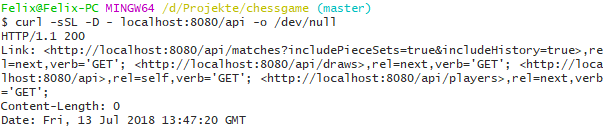
\includegraphics[width=0.8\textwidth]{images/question3.1.png}
			\item curl -sSL -D - localhost:8080/api/players -o /dev/null\\
				\\
				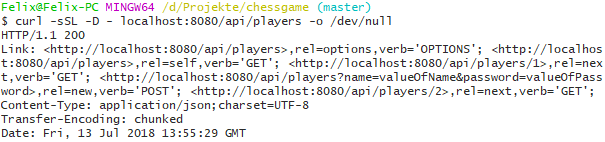
\includegraphics[width=0.8\textwidth]{images/question3.2.png}
			\item curl -sSL -D - localhost:8080/api/players/2 -o /dev/null\\
				\\
				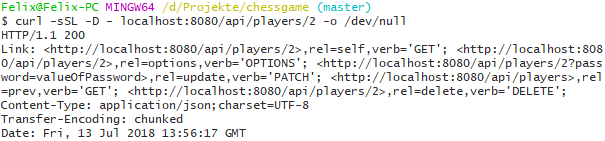
\includegraphics[width=0.8\textwidth]{images/question3.3.png}
			\item curl -sSL -D - localhost:8080/api/players -o/dev/null
			\item curl -sSL -D - localhost:8080/api -o /dev/null
			\item curl -sSL -D - localhost:8080/api/matches -o /dev/null\\
				\\
				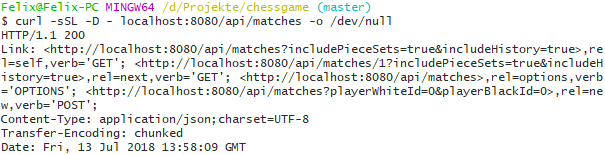
\includegraphics[width=0.8\textwidth]{images/question3.6.png}
			\newpage
			\item curl -sSL -D - localhost:8080/api/matches/1 -o /dev/null\\
				\\
				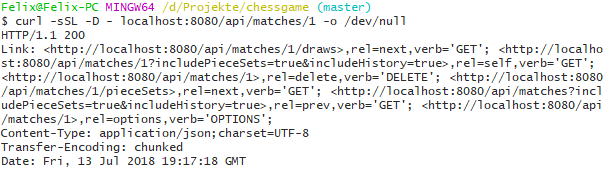
\includegraphics[width=0.8\textwidth]{images/question3.7.png}
			\item curl -sSL -D - localhost:8080/api/matches/1/draws -o /dev/null\\
				\\
				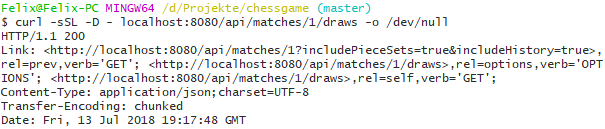
\includegraphics[width=0.8\textwidth]{images/question3.8.png}
			\item curl -sSL -D - localhost:8080/api/matches/1 -o /dev/null
			\item curl -sSL -D - localhost:8080/api/matches/1/pieceSets -o /dev/null\\
				\\
				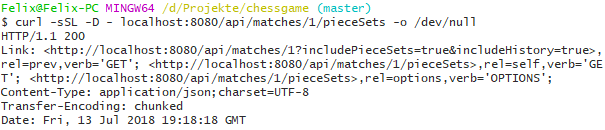
\includegraphics[width=0.8\textwidth]{images/question3.10.png}
			\item curl -sSL -D - localhost:8080/api/matches/1 -o /dev/null
			\item curl -sSL -D - localhost:8080/api/matches -o /dev/null
			\item curl -sSL -D - localhost:8080/api -o /dev/null
			\item curl -sSL -D - localhost:8080/api/draws -o /dev/null\\
				\\
				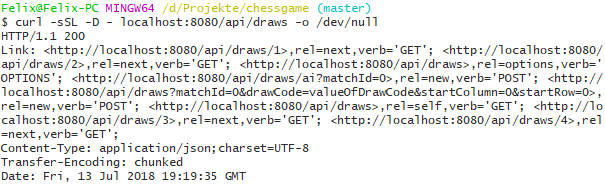
\includegraphics[width=0.8\textwidth]{images/question3.14.png}
			\newpage
			\item curl -sSL -D - localhost:8080/api/draws/1 -o /dev/null\\
				\\
				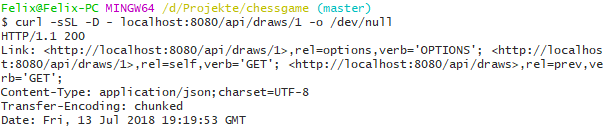
\includegraphics[width=0.8\textwidth]{images/question3.15.png}
			\item curl -sSL -D - localhost:8080/api/draws -o /dev/null
			\item curl -sSL -D - localhost:8080/api -o /dev/null
		\end{itemize}
	\item Anlegen neuer Player
		\begin{itemize}
			\item curl -v -H \textquotesingle Content-Type: application/x-www-form-urlencoded\textquotesingle\\-d \textquotesingle name=Test\&password=123456\textquotesingle\ localhost:8080/api/players\\
				\\
				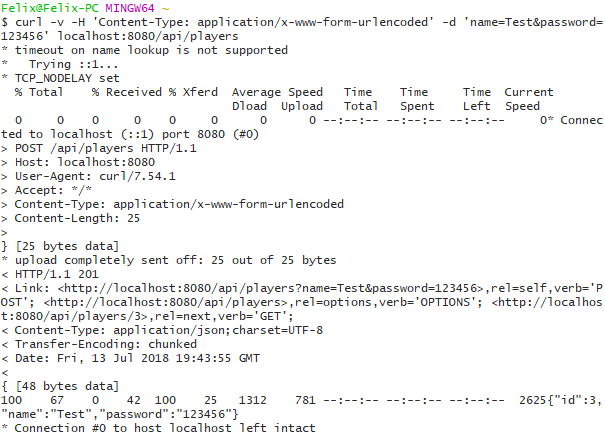
\includegraphics[width=0.8\textwidth]{images/question4.1.png}
			\newpage
			\item curl -v -H \textquotesingle Content-Type: application/json\textquotesingle\\-d \textquotesingle\{ "name": "Test", "password": "123456"\ \}\textquotesingle\ localhost:8080/api/players\\
				\\
				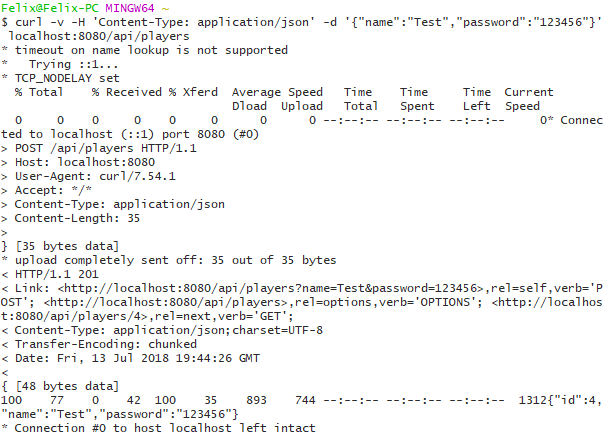
\includegraphics[width=0.8\textwidth]{images/question4.2.png}
		\end{itemize}
	\item Aktualisierung eines Players
		\begin{itemize}
			\item curl -v -X PATCH -H \textquotesingle Content-Type: application/json\textquotesingle\\-d \textquotesingle\{ "password": "987654"\ \}\textquotesingle\ localhost:8080/api/players/3\\
				\\
				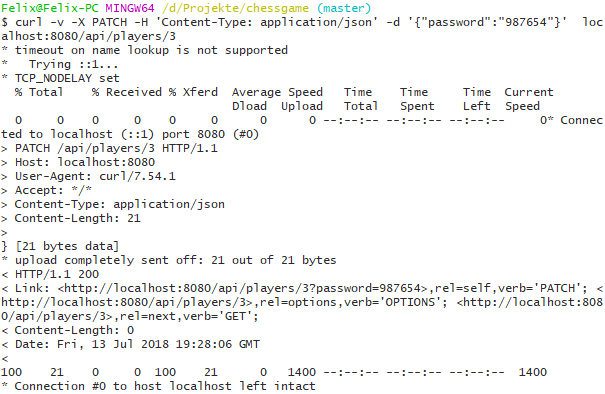
\includegraphics[width=0.8\textwidth]{images/question5.png}
		\end{itemize}
	\newpage
	\item Löschen eines Players
		\begin{itemize}
			\item curl -v -X DELETE localhost:8080/api/players/3\\
				\\
				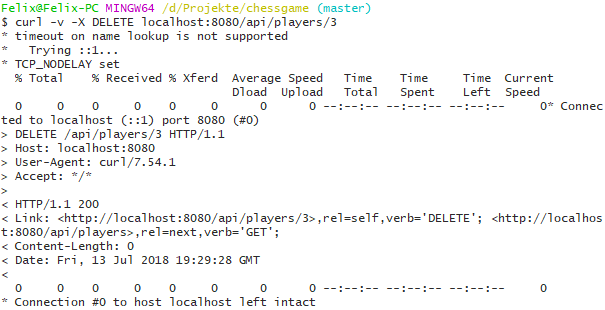
\includegraphics[width=0.8\textwidth]{images/question6.png}
		\end{itemize}
	\newpage
	\item Anlegen eines neuen Matches
		\begin{itemize}
			\item curl -v -H \textquotesingle Content-Type: application/json\textquotesingle\\-d \textquotesingle\{ "playerWhiteId": 1, "playerBlackId": 2\ \}\textquotesingle\ localhost:8080/api/matches\\
				\\
				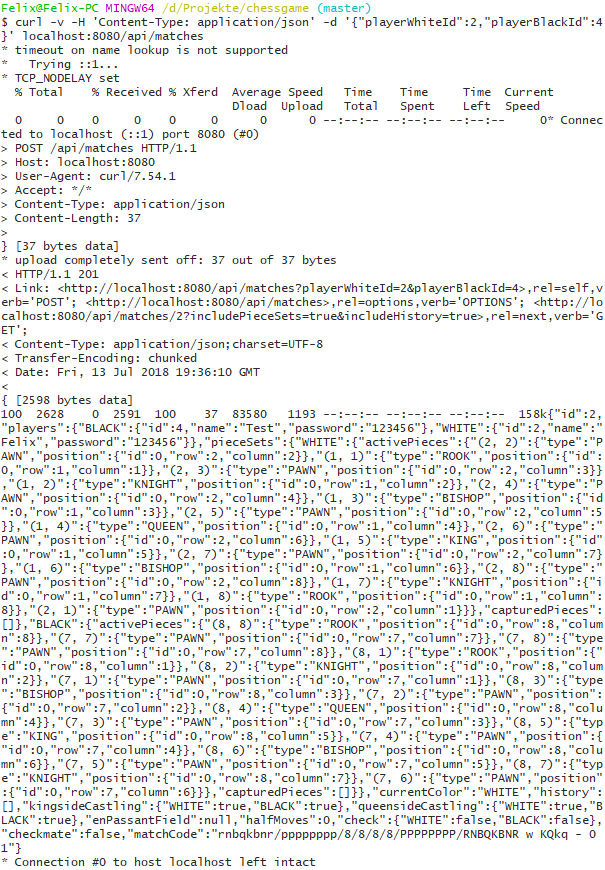
\includegraphics[width=0.8\textwidth]{images/question7.png}
		\end{itemize}
	\newpage
	\item Anlegen neuer Draws
		\begin{itemize}
			\item curl -v -H \textquotesingle Content-Type: application/json\textquotesingle\\-d \textquotesingle\{ "matchId": 2, "drawCode": \textquotesingle\textquotesingle e4", \textquotesingle\textquotesingle startColumn": 5, \textquotesingle\textquotesingle startRow": 2\ \}\textquotesingle\\localhost:8080/api/draws\\
				\\
				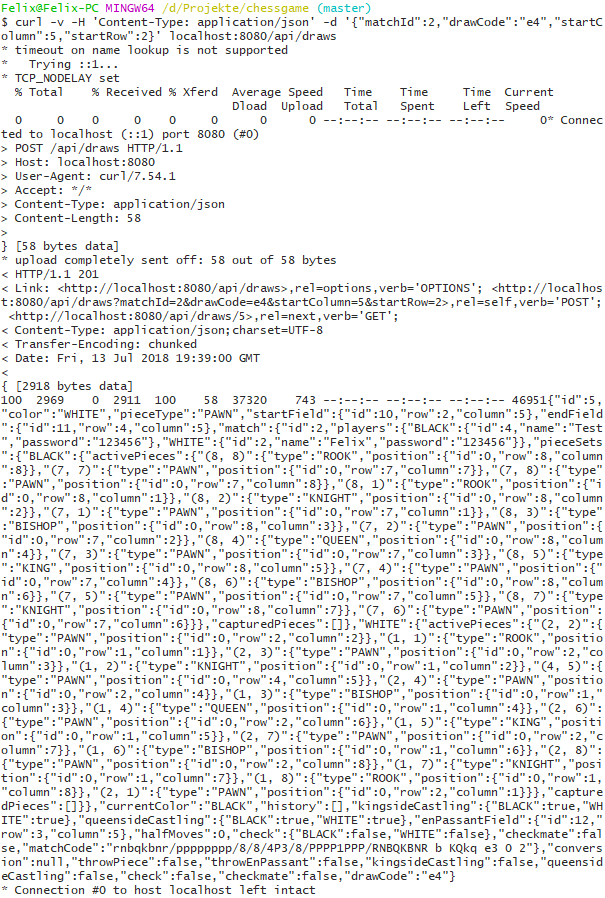
\includegraphics[width=0.8\textwidth]{images/question8.1.png}
			\newpage
			\item curl -v -H \textquotesingle Content-Type: application/json\textquotesingle\\-d \textquotesingle \{ "matchId": 2, "drawCode": "d5", \textquotesingle\textquotesingle startColumn": 4, \textquotesingle\textquotesingle startRow": 7\ \}\textquotesingle\\localhost:8080/api/draws\\
				\\
				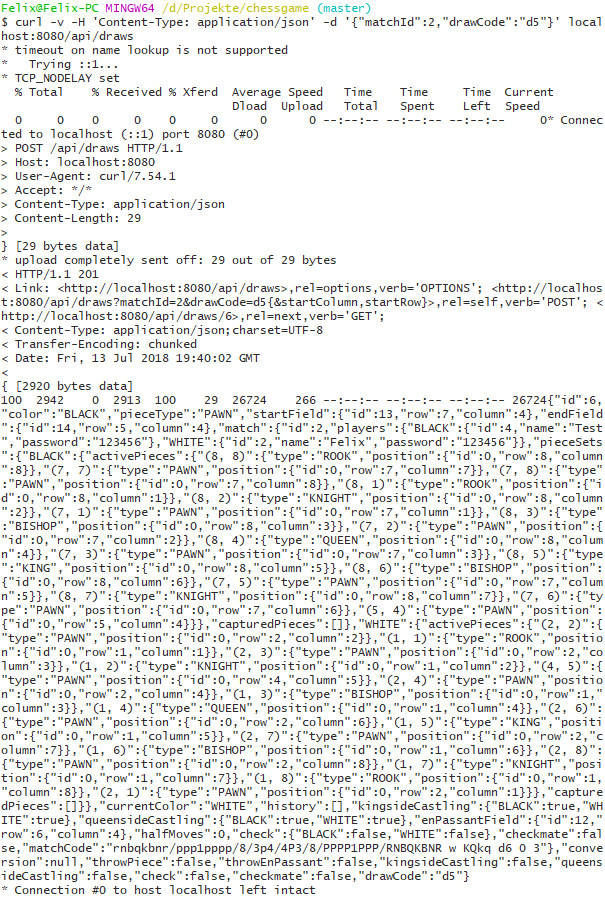
\includegraphics[width=0.8\textwidth]{images/question8.2.png}
			\newpage
			\item curl -v -H \textquotesingle Content-Type: application/json\textquotesingle\\-d \textquotesingle \{ "matchId": 2, "drawCode": \textquotesingle\textquotesingle exd5", \textquotesingle\textquotesingle startColumn": 5, \textquotesingle\textquotesingle startRow": 4\ \}\textquotesingle\\localhost:8080/api/draws\\
				\\
				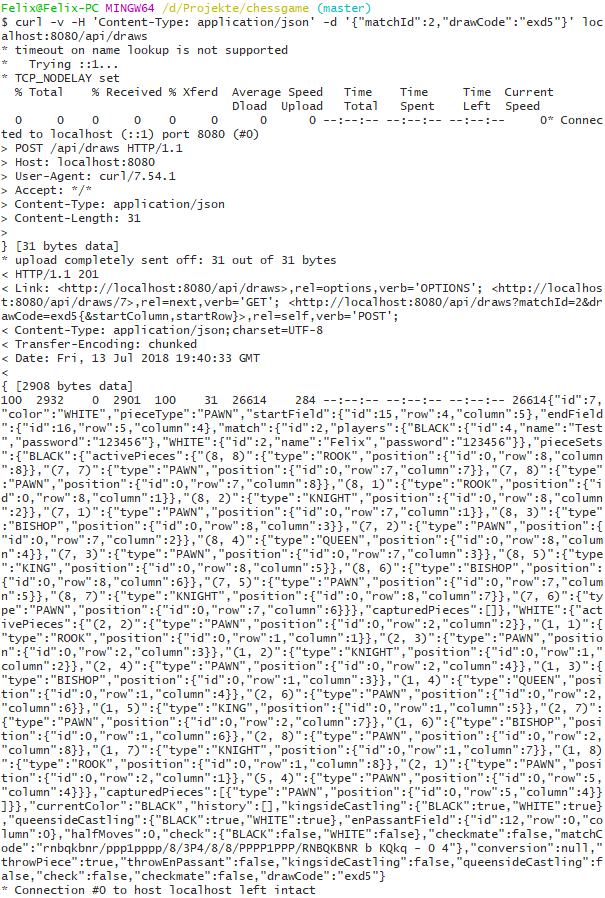
\includegraphics[width=0.8\textwidth]{images/question8.3.png}
		\end{itemize}
\end{enumerate}


%% -- Index --
% _Remove_ Index unless you really want to invest a large amount
% of time and effort to create a good index!
\IfDefined{printindex}{%
  \cleardoublepage\IfDefined{phantomsection}{\phantomsection}\label{sec:index}%
  \printindex%
}% end of index

%%% document END %%%%%%%%%%%%%%%%%%%%%%%%%%%%%%%%%%%%%%%%%%%%%%%%%%%%%%%%%%%
\end{document}
%%%%%%%%%%%%%%%%%%%%%%%%%%%%%%%%%%%%%%%%%%%%%%%%%%%%%%%%%%%%%%%%%%%%%%%%%%%%